\documentclass[11pt, a4paper]{article}
\usepackage{epsfig}
\usepackage{graphicx}
\usepackage{subfigure}
\usepackage{amssymb, amsmath, amsthm, mathtools}
\usepackage[margin=2.5cm]{geometry}
\usepackage{tikz}
\usepackage{siunitx}
\usepackage{booktabs}
\usepackage{caption}
\usepackage{pgfplots}
\usepackage{listings}
\usepackage{caption}

\makeatletter
\def\fps@figure{hbtp}
\def\fps@table{hbtp}
\makeatother

\let\originalleft\left
\let\originalright\right
\renewcommand{\left}{\mathopen{}\mathclose\bgroup\originalleft}
\renewcommand{\right}{\aftergroup\egroup\originalright}

\DeclareMathOperator{\Normal}{Normal}
\DeclareMathOperator{\GammaD}{Gamma}
\DeclareMathOperator{\Bernoulli}{Bernoulli}
\DeclareMathOperator{\mean}{mean}
\DeclareMathOperator{\var}{var}

\lstset{
	breaklines=true,
	postbreak=\mbox{\textcolor{red}{$\hookrightarrow$}\space},
	}

\title{Assignment 4}
\author{Axel Forsman}

\begin{document}
\maketitle

\section{Introduction}

\section{Assignment 1(a)}\label{sec:max_proof}
\subsection{Problem}
Prove that $\mathbb E[u(t)]$ is maximized as a function of
$\mu$ and $\sigma^2$ when $\mu - k\sigma^2/2$ is maximized.
\subsection{Theory and implementation}
The utility function $u$ is defined as
\begin{equation}\label{eq:utility}
u(x) = \frac{1 - (x / K)^{-k}}k
\end{equation}
where $k \neq 0$ is a parameter and $K$ is the amount invested.
\subsection{Results and discussion}
\begin{align*}
	\mathbb E[u(t)] &= \int_\infty^\infty \frac{1 - e^{-yk}}k \frac1{\sqrt{2\pi\sigma^2}}
		\exp\left(-\frac1{2\sigma^2} (y - \mu)^2\right) \, dy \\
		&= \frac1k \left(\underbrace{\int_\infty^\infty \frac1{\sqrt{2\pi\sigma^2}} \exp\left(-\frac1{2\sigma^2} (y - \mu)^2\right) \, dy}_{=1, \, \text{for integral of pdf of normal distribution}}
		- \int_\infty^\infty e^{-yk} \frac1{\sqrt{2\pi\sigma^2}} \exp\left(-\frac1{2\sigma^2} (y - \mu)^2\right) \, dy\right) \\
		&= \frac1k \left(1 - \int_\infty^\infty \frac1{\sqrt{2\pi\sigma^2}}
			\exp\left(\underbrace{-yk - \frac1{2\sigma^2} (y - \mu)^2}_{\begin{subarray}{1}
				= y^2 - 2y(\mu - \sigma^2k) + \mu^2 \\
				= (y - (\mu - \sigma^2k))^2 + 2\sigma^2k\mu - (\sigma^2k)^2
			\end{subarray}}\right) \, dy\right) \\
		&= \frac1k \left(1 - \exp\left(-\frac{2\sigma^2k\mu - (\sigma^2k)^2}{2\sigma^2}\right)
			\int_\infty^\infty \frac1{\sqrt{2\pi\sigma^2}} \exp\left(-\frac1{2\sigma^2} (y - (\mu - \sigma^2k))^2\right) \, dy\right) \\
		&= \frac1k \left(1 - \exp\left(-k \left(\mu - \frac{k\sigma^2}2\right)\right)\right)
\end{align*}
which is maximized when $\mu - k\sigma^2/2$ is maximized, since
$\left(1 - \exp\left(-k x\right)\right) / k$
is an increasing function of $x$, regardless of $k \ne 0$.

\section{Assignment 1(b)}
\subsection{Problem}
Optimize the weights in the case of two stocks,
using the utility function from equation~\ref{eq:utility}.
\subsection{Theory and implementation}
With $X_{ij}$ as the closing price of stock $i$ after day $j$ we define
$$ Z_{ij} \coloneqq \log\left(\frac{X_{ij}}{X_{i,j-1}}\right) $$
as the relative change in stock price from day to day,
we say that the vectors $Z_j$ are independent and
$$ Z_j \sim \Normal(\gamma, \Sigma) $$
for some vector $\gamma$ and covariance matrix $\Sigma$.
Choosing a set of weights $w = (w_1, \ldots, w_k), \quad \sum_{i=1}^k w_i = 1$,
we define
$$ T = K \prod_{i=1}^k \exp(w_i n Z_i) = K \exp\left(\sum_{i=1}^k w_i n Z_i\right)
	= K \exp(n w^T Z) = K \exp(Y) $$
where $T$ is the total amount after $n$ days, given an amount $K$ invested,
and $Y \coloneqq n w^T Z$.
Now
$$ Y \sim \Normal(n w^T \gamma, n w^T \Sigma w) = \Normal(\gamma, \sigma^2) $$
with the added notation
$\gamma \coloneqq n w^T \gamma$ and $\sigma^2 \coloneqq n w^T \Sigma w$.

Decision theory tells us that we should pick the weights $w$ so that
$\mathbb E[u(T)]$ is maximized.
But in section~\ref{sec:max_proof} we saw that this is equivalent to maximizing
$$ F(w) = \mu - k \sigma^2 / 2 $$

The R function \texttt{optim} is used to maximize.
\subsection{Results and discussion}
The optimized stock weight is shown in figure~\ref{fig:stock_weights}.
We see that the \texttt{Comp1} ratio decreases with $k$,
which should imply that \texttt{Comp1} is more instable
- it is also the case that
$\num{553.2989} = \var(\text{\texttt{Comp1}}) > \var(\text{\texttt{Comp2}}) = \num{382.5174}$.
Expanding $F(w) = n w^T \gamma - k n w^T \Sigma w / 2$
we see that the second term is conserned with variability,
while the first term rewards weighting stocks with higher mean change more heavily.
Thus \texttt{Comp1} is favored more overall for the observed values of $k$
since $\num{0.0005275481} = \mean(Z_{1,:}) > \mean(Z_{2,:}) = \num{0.0001782805}$.

\begin{figure}
	\centering
	% Created by tikzDevice version 0.12.3 on 2019-10-10 21:33:38
% !TEX encoding = UTF-8 Unicode
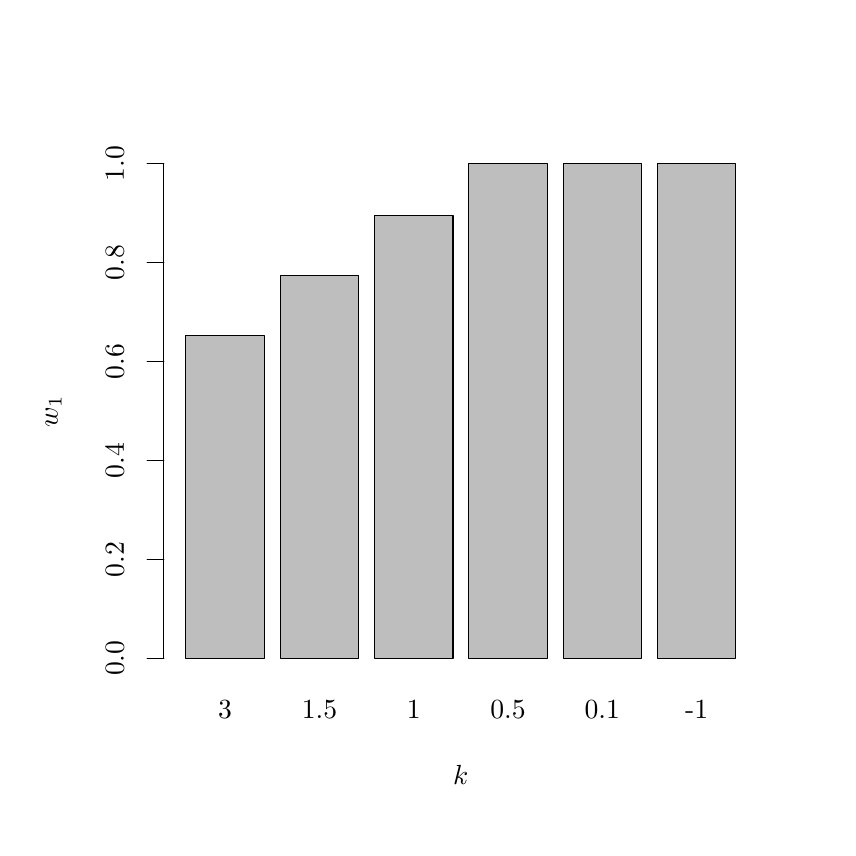
\begin{tikzpicture}[x=1pt,y=1pt]
\definecolor{fillColor}{RGB}{255,255,255}
\path[use as bounding box,fill=fillColor,fill opacity=0.00] (0,0) rectangle (289.08,289.08);
\begin{scope}
\path[clip] (  0.00,  0.00) rectangle (289.08,289.08);
\definecolor{drawColor}{RGB}{0,0,0}
\definecolor{fillColor}{RGB}{190,190,190}

\path[draw=drawColor,line width= 0.4pt,line join=round,line cap=round,fill=fillColor] ( 57.15, 61.20) rectangle ( 85.55,177.81);

\path[draw=drawColor,line width= 0.4pt,line join=round,line cap=round,fill=fillColor] ( 91.23, 61.20) rectangle (119.62,199.53);

\path[draw=drawColor,line width= 0.4pt,line join=round,line cap=round,fill=fillColor] (125.30, 61.20) rectangle (153.70,221.25);

\path[draw=drawColor,line width= 0.4pt,line join=round,line cap=round,fill=fillColor] (159.38, 61.20) rectangle (187.78,239.87);

\path[draw=drawColor,line width= 0.4pt,line join=round,line cap=round,fill=fillColor] (193.46, 61.20) rectangle (221.85,239.87);

\path[draw=drawColor,line width= 0.4pt,line join=round,line cap=round,fill=fillColor] (227.53, 61.20) rectangle (255.93,239.87);
\end{scope}
\begin{scope}
\path[clip] (  0.00,  0.00) rectangle (289.08,289.08);
\definecolor{drawColor}{RGB}{0,0,0}

\node[text=drawColor,anchor=base,inner sep=0pt, outer sep=0pt, scale=  1.00] at ( 71.35, 39.60) {3};

\node[text=drawColor,anchor=base,inner sep=0pt, outer sep=0pt, scale=  1.00] at (105.43, 39.60) {1.5};

\node[text=drawColor,anchor=base,inner sep=0pt, outer sep=0pt, scale=  1.00] at (139.50, 39.60) {1};

\node[text=drawColor,anchor=base,inner sep=0pt, outer sep=0pt, scale=  1.00] at (173.58, 39.60) {0.5};

\node[text=drawColor,anchor=base,inner sep=0pt, outer sep=0pt, scale=  1.00] at (207.65, 39.60) {0.1};

\node[text=drawColor,anchor=base,inner sep=0pt, outer sep=0pt, scale=  1.00] at (241.73, 39.60) {-1};
\end{scope}
\begin{scope}
\path[clip] (  0.00,  0.00) rectangle (289.08,289.08);
\definecolor{drawColor}{RGB}{0,0,0}

\node[text=drawColor,anchor=base,inner sep=0pt, outer sep=0pt, scale=  1.00] at (156.54, 15.60) {$k$};

\node[text=drawColor,rotate= 90.00,anchor=base,inner sep=0pt, outer sep=0pt, scale=  1.00] at ( 10.80,150.54) {$w_1$};
\end{scope}
\begin{scope}
\path[clip] (  0.00,  0.00) rectangle (289.08,289.08);
\definecolor{drawColor}{RGB}{0,0,0}

\path[draw=drawColor,line width= 0.4pt,line join=round,line cap=round] ( 49.20, 61.20) -- ( 49.20,239.88);

\path[draw=drawColor,line width= 0.4pt,line join=round,line cap=round] ( 49.20, 61.20) -- ( 43.20, 61.20);

\path[draw=drawColor,line width= 0.4pt,line join=round,line cap=round] ( 49.20, 96.94) -- ( 43.20, 96.94);

\path[draw=drawColor,line width= 0.4pt,line join=round,line cap=round] ( 49.20,132.67) -- ( 43.20,132.67);

\path[draw=drawColor,line width= 0.4pt,line join=round,line cap=round] ( 49.20,168.41) -- ( 43.20,168.41);

\path[draw=drawColor,line width= 0.4pt,line join=round,line cap=round] ( 49.20,204.14) -- ( 43.20,204.14);

\path[draw=drawColor,line width= 0.4pt,line join=round,line cap=round] ( 49.20,239.88) -- ( 43.20,239.88);

\node[text=drawColor,rotate= 90.00,anchor=base,inner sep=0pt, outer sep=0pt, scale=  1.00] at ( 34.80, 61.20) {0.0};

\node[text=drawColor,rotate= 90.00,anchor=base,inner sep=0pt, outer sep=0pt, scale=  1.00] at ( 34.80, 96.94) {0.2};

\node[text=drawColor,rotate= 90.00,anchor=base,inner sep=0pt, outer sep=0pt, scale=  1.00] at ( 34.80,132.67) {0.4};

\node[text=drawColor,rotate= 90.00,anchor=base,inner sep=0pt, outer sep=0pt, scale=  1.00] at ( 34.80,168.41) {0.6};

\node[text=drawColor,rotate= 90.00,anchor=base,inner sep=0pt, outer sep=0pt, scale=  1.00] at ( 34.80,204.14) {0.8};

\node[text=drawColor,rotate= 90.00,anchor=base,inner sep=0pt, outer sep=0pt, scale=  1.00] at ( 34.80,239.88) {1.0};
\end{scope}
\end{tikzpicture}

	\caption{Plot of the optimized stock weight,
		that is the ratio that should be invested in \texttt{Comp1},
	for different values of $k$. \label{fig:stock_weights}}
\end{figure}

\section{Assignment 2(a)}
\subsection{Problem}
Fit a logistic regression to the data, by numerical maximum likelihood
given parameters $a$ and $b$.
\subsection{Theory and implementation}
There are two reports
$$ \text{reports} = \left\{\underbrace{\text{mature}}_1, \underbrace{\text{immature}}_0\right\} $$
Our model is
$$ y \sim \Bernoulli(f_1(x)), \quad f_1(x) = \frac{\exp\left(a + b (x - 18)\right)}{1 + \exp\left(a + b (x - 18)\right)} $$
$a, b \in \mathbb R$.
The likelihood is given by
$$ \mathcal L(a, b) = \prod_{\text{mature}} f_1(x) \prod_{\text{immature}} f_0(x) $$
\subsection{Results and discussion}
The fitted logistic regression curve is shown in figure~\ref{fig:logistic_regression}.
We see that the result seems plausible since the location where the curve
changes from $0$ to $1$ happens in the middle of the two datasets.

\begin{figure}
	\centering
	% Created by tikzDevice version 0.12.3 on 2019-10-13 21:26:54
% !TEX encoding = UTF-8 Unicode
\begin{tikzpicture}[x=1pt,y=1pt]
\definecolor{fillColor}{RGB}{255,255,255}
\path[use as bounding box,fill=fillColor,fill opacity=0.00] (0,0) rectangle (361.35,361.35);
\begin{scope}
\path[clip] ( 49.20, 61.20) rectangle (336.15,312.15);
\definecolor{drawColor}{RGB}{0,0,0}

\path[draw=drawColor,line width= 0.4pt,line join=round,line cap=round] ( 59.83, 70.49) --
	( 60.36, 70.49) --
	( 60.89, 70.49) --
	( 61.43, 70.49) --
	( 61.96, 70.49) --
	( 62.49, 70.49) --
	( 63.02, 70.49) --
	( 63.55, 70.49) --
	( 64.09, 70.49) --
	( 64.62, 70.49) --
	( 65.15, 70.49) --
	( 65.68, 70.49) --
	( 66.22, 70.49) --
	( 66.75, 70.49) --
	( 67.28, 70.49) --
	( 67.81, 70.49) --
	( 68.35, 70.49) --
	( 68.88, 70.49) --
	( 69.41, 70.49) --
	( 69.94, 70.49) --
	( 70.48, 70.49) --
	( 71.01, 70.49) --
	( 71.54, 70.49) --
	( 72.07, 70.49) --
	( 72.61, 70.49) --
	( 73.14, 70.49) --
	( 73.67, 70.49) --
	( 74.20, 70.49) --
	( 74.74, 70.49) --
	( 75.27, 70.49) --
	( 75.80, 70.49) --
	( 76.33, 70.49) --
	( 76.87, 70.49) --
	( 77.40, 70.49) --
	( 77.93, 70.49) --
	( 78.46, 70.49) --
	( 79.00, 70.49) --
	( 79.53, 70.49) --
	( 80.06, 70.49) --
	( 80.59, 70.49) --
	( 81.13, 70.49) --
	( 81.66, 70.49) --
	( 82.19, 70.49) --
	( 82.72, 70.49) --
	( 83.26, 70.49) --
	( 83.79, 70.49) --
	( 84.32, 70.49) --
	( 84.85, 70.49) --
	( 85.39, 70.49) --
	( 85.92, 70.49) --
	( 86.45, 70.49) --
	( 86.98, 70.49) --
	( 87.52, 70.49) --
	( 88.05, 70.49) --
	( 88.58, 70.49) --
	( 89.11, 70.49) --
	( 89.65, 70.49) --
	( 90.18, 70.49) --
	( 90.71, 70.49) --
	( 91.24, 70.49) --
	( 91.78, 70.49) --
	( 92.31, 70.49) --
	( 92.84, 70.49) --
	( 93.37, 70.49) --
	( 93.90, 70.49) --
	( 94.44, 70.49) --
	( 94.97, 70.49) --
	( 95.50, 70.49) --
	( 96.03, 70.49) --
	( 96.57, 70.49) --
	( 97.10, 70.49) --
	( 97.63, 70.49) --
	( 98.16, 70.49) --
	( 98.70, 70.49) --
	( 99.23, 70.49) --
	( 99.76, 70.49) --
	(100.29, 70.49) --
	(100.83, 70.49) --
	(101.36, 70.49) --
	(101.89, 70.49) --
	(102.42, 70.49) --
	(102.96, 70.49) --
	(103.49, 70.49) --
	(104.02, 70.49) --
	(104.55, 70.49) --
	(105.09, 70.49) --
	(105.62, 70.49) --
	(106.15, 70.49) --
	(106.68, 70.49) --
	(107.22, 70.49) --
	(107.75, 70.49) --
	(108.28, 70.49) --
	(108.81, 70.49) --
	(109.35, 70.49) --
	(109.88, 70.49) --
	(110.41, 70.49) --
	(110.94, 70.49) --
	(111.48, 70.49) --
	(112.01, 70.49) --
	(112.54, 70.49) --
	(113.07, 70.49) --
	(113.61, 70.49) --
	(114.14, 70.49) --
	(114.67, 70.49) --
	(115.20, 70.49) --
	(115.74, 70.49) --
	(116.27, 70.49) --
	(116.80, 70.49) --
	(117.33, 70.49) --
	(117.87, 70.49) --
	(118.40, 70.49) --
	(118.93, 70.49) --
	(119.46, 70.49) --
	(120.00, 70.49) --
	(120.53, 70.49) --
	(121.06, 70.49) --
	(121.59, 70.49) --
	(122.12, 70.49) --
	(122.66, 70.49) --
	(123.19, 70.49) --
	(123.72, 70.49) --
	(124.25, 70.49) --
	(124.79, 70.49) --
	(125.32, 70.49) --
	(125.85, 70.49) --
	(126.38, 70.49) --
	(126.92, 70.50) --
	(127.45, 70.50) --
	(127.98, 70.50) --
	(128.51, 70.50) --
	(129.05, 70.50) --
	(129.58, 70.50) --
	(130.11, 70.50) --
	(130.64, 70.50) --
	(131.18, 70.50) --
	(131.71, 70.50) --
	(132.24, 70.50) --
	(132.77, 70.50) --
	(133.31, 70.50) --
	(133.84, 70.50) --
	(134.37, 70.50) --
	(134.90, 70.50) --
	(135.44, 70.50) --
	(135.97, 70.50) --
	(136.50, 70.50) --
	(137.03, 70.50) --
	(137.57, 70.50) --
	(138.10, 70.50) --
	(138.63, 70.51) --
	(139.16, 70.51) --
	(139.70, 70.51) --
	(140.23, 70.51) --
	(140.76, 70.52) --
	(141.29, 70.52) --
	(141.83, 70.52) --
	(142.36, 70.53) --
	(142.89, 70.53) --
	(143.42, 70.54) --
	(143.96, 70.54) --
	(144.49, 70.55) --
	(145.02, 70.56) --
	(145.55, 70.57) --
	(146.09, 70.58) --
	(146.62, 70.59) --
	(147.15, 70.60) --
	(147.68, 70.62) --
	(148.22, 70.64) --
	(148.75, 70.66) --
	(149.28, 70.68) --
	(149.81, 70.71) --
	(150.34, 70.74) --
	(150.88, 70.78) --
	(151.41, 70.82) --
	(151.94, 70.87) --
	(152.47, 70.92) --
	(153.01, 70.99) --
	(153.54, 71.06) --
	(154.07, 71.14) --
	(154.60, 71.24) --
	(155.14, 71.35) --
	(155.67, 71.48) --
	(156.20, 71.62) --
	(156.73, 71.79) --
	(157.27, 71.97) --
	(157.80, 72.19) --
	(158.33, 72.44) --
	(158.86, 72.73) --
	(159.40, 73.05) --
	(159.93, 73.43) --
	(160.46, 73.86) --
	(160.99, 74.34) --
	(161.53, 74.90) --
	(162.06, 75.54) --
	(162.59, 76.27) --
	(163.12, 77.10) --
	(163.66, 78.05) --
	(164.19, 79.12) --
	(164.72, 80.35) --
	(165.25, 81.73) --
	(165.79, 83.31) --
	(166.32, 85.08) --
	(166.85, 87.09) --
	(167.38, 89.34) --
	(167.92, 91.88) --
	(168.45, 94.71) --
	(168.98, 97.87) --
	(169.51,101.38) --
	(170.05,105.27) --
	(170.58,109.55) --
	(171.11,114.25) --
	(171.64,119.36) --
	(172.18,124.90) --
	(172.71,130.86) --
	(173.24,137.22) --
	(173.77,143.98) --
	(174.31,151.08) --
	(174.84,158.49) --
	(175.37,166.15) --
	(175.90,174.00) --
	(176.44,181.97) --
	(176.97,189.98) --
	(177.50,197.97) --
	(178.03,205.84) --
	(178.56,213.54) --
	(179.10,221.00) --
	(179.63,228.16) --
	(180.16,234.97) --
	(180.69,241.41) --
	(181.23,247.44) --
	(181.76,253.06) --
	(182.29,258.24) --
	(182.82,263.01) --
	(183.36,267.36) --
	(183.89,271.31) --
	(184.42,274.89) --
	(184.95,278.11) --
	(185.49,281.00) --
	(186.02,283.59) --
	(186.55,285.89) --
	(187.08,287.94) --
	(187.62,289.75) --
	(188.15,291.36) --
	(188.68,292.77) --
	(189.21,294.02) --
	(189.75,295.12) --
	(190.28,296.09) --
	(190.81,296.94) --
	(191.34,297.69) --
	(191.88,298.34) --
	(192.41,298.91) --
	(192.94,299.41) --
	(193.47,299.85) --
	(194.01,300.23) --
	(194.54,300.57) --
	(195.07,300.86) --
	(195.60,301.12) --
	(196.14,301.34) --
	(196.67,301.53) --
	(197.20,301.70) --
	(197.73,301.85) --
	(198.27,301.98) --
	(198.80,302.09) --
	(199.33,302.19) --
	(199.86,302.28) --
	(200.40,302.35) --
	(200.93,302.42) --
	(201.46,302.47) --
	(201.99,302.52) --
	(202.53,302.56) --
	(203.06,302.60) --
	(203.59,302.63) --
	(204.12,302.66) --
	(204.66,302.69) --
	(205.19,302.71) --
	(205.72,302.73) --
	(206.25,302.74) --
	(206.79,302.76) --
	(207.32,302.77) --
	(207.85,302.78) --
	(208.38,302.79) --
	(208.91,302.80) --
	(209.45,302.81) --
	(209.98,302.81) --
	(210.51,302.82) --
	(211.04,302.82) --
	(211.58,302.83) --
	(212.11,302.83) --
	(212.64,302.83) --
	(213.17,302.84) --
	(213.71,302.84) --
	(214.24,302.84) --
	(214.77,302.84) --
	(215.30,302.84) --
	(215.84,302.85) --
	(216.37,302.85) --
	(216.90,302.85) --
	(217.43,302.85) --
	(217.97,302.85) --
	(218.50,302.85) --
	(219.03,302.85) --
	(219.56,302.85) --
	(220.10,302.85) --
	(220.63,302.85) --
	(221.16,302.85) --
	(221.69,302.85) --
	(222.23,302.85) --
	(222.76,302.85) --
	(223.29,302.85) --
	(223.82,302.85) --
	(224.36,302.85) --
	(224.89,302.85) --
	(225.42,302.85) --
	(225.95,302.85) --
	(226.49,302.85) --
	(227.02,302.86) --
	(227.55,302.86) --
	(228.08,302.86) --
	(228.62,302.86) --
	(229.15,302.86) --
	(229.68,302.86) --
	(230.21,302.86) --
	(230.75,302.86) --
	(231.28,302.86) --
	(231.81,302.86) --
	(232.34,302.86) --
	(232.88,302.86) --
	(233.41,302.86) --
	(233.94,302.86) --
	(234.47,302.86) --
	(235.01,302.86) --
	(235.54,302.86) --
	(236.07,302.86) --
	(236.60,302.86) --
	(237.13,302.86) --
	(237.67,302.86) --
	(238.20,302.86) --
	(238.73,302.86) --
	(239.26,302.86) --
	(239.80,302.86) --
	(240.33,302.86) --
	(240.86,302.86) --
	(241.39,302.86) --
	(241.93,302.86) --
	(242.46,302.86) --
	(242.99,302.86) --
	(243.52,302.86) --
	(244.06,302.86) --
	(244.59,302.86) --
	(245.12,302.86) --
	(245.65,302.86) --
	(246.19,302.86) --
	(246.72,302.86) --
	(247.25,302.86) --
	(247.78,302.86) --
	(248.32,302.86) --
	(248.85,302.86) --
	(249.38,302.86) --
	(249.91,302.86) --
	(250.45,302.86) --
	(250.98,302.86) --
	(251.51,302.86) --
	(252.04,302.86) --
	(252.58,302.86) --
	(253.11,302.86) --
	(253.64,302.86) --
	(254.17,302.86) --
	(254.71,302.86) --
	(255.24,302.86) --
	(255.77,302.86) --
	(256.30,302.86) --
	(256.84,302.86) --
	(257.37,302.86) --
	(257.90,302.86) --
	(258.43,302.86) --
	(258.97,302.86) --
	(259.50,302.86) --
	(260.03,302.86) --
	(260.56,302.86) --
	(261.10,302.86) --
	(261.63,302.86) --
	(262.16,302.86) --
	(262.69,302.86) --
	(263.23,302.86) --
	(263.76,302.86) --
	(264.29,302.86) --
	(264.82,302.86) --
	(265.35,302.86) --
	(265.89,302.86) --
	(266.42,302.86) --
	(266.95,302.86) --
	(267.48,302.86) --
	(268.02,302.86) --
	(268.55,302.86) --
	(269.08,302.86) --
	(269.61,302.86) --
	(270.15,302.86) --
	(270.68,302.86) --
	(271.21,302.86) --
	(271.74,302.86) --
	(272.28,302.86) --
	(272.81,302.86) --
	(273.34,302.86) --
	(273.87,302.86) --
	(274.41,302.86) --
	(274.94,302.86) --
	(275.47,302.86) --
	(276.00,302.86) --
	(276.54,302.86) --
	(277.07,302.86) --
	(277.60,302.86) --
	(278.13,302.86) --
	(278.67,302.86) --
	(279.20,302.86) --
	(279.73,302.86) --
	(280.26,302.86) --
	(280.80,302.86) --
	(281.33,302.86) --
	(281.86,302.86) --
	(282.39,302.86) --
	(282.93,302.86) --
	(283.46,302.86) --
	(283.99,302.86) --
	(284.52,302.86) --
	(285.06,302.86) --
	(285.59,302.86) --
	(286.12,302.86) --
	(286.65,302.86) --
	(287.19,302.86) --
	(287.72,302.86) --
	(288.25,302.86) --
	(288.78,302.86) --
	(289.32,302.86) --
	(289.85,302.86) --
	(290.38,302.86) --
	(290.91,302.86) --
	(291.45,302.86) --
	(291.98,302.86) --
	(292.51,302.86) --
	(293.04,302.86) --
	(293.57,302.86) --
	(294.11,302.86) --
	(294.64,302.86) --
	(295.17,302.86) --
	(295.70,302.86) --
	(296.24,302.86) --
	(296.77,302.86) --
	(297.30,302.86) --
	(297.83,302.86) --
	(298.37,302.86) --
	(298.90,302.86) --
	(299.43,302.86) --
	(299.96,302.86) --
	(300.50,302.86) --
	(301.03,302.86) --
	(301.56,302.86) --
	(302.09,302.86) --
	(302.63,302.86) --
	(303.16,302.86) --
	(303.69,302.86) --
	(304.22,302.86) --
	(304.76,302.86) --
	(305.29,302.86) --
	(305.82,302.86) --
	(306.35,302.86) --
	(306.89,302.86) --
	(307.42,302.86) --
	(307.95,302.86) --
	(308.48,302.86) --
	(309.02,302.86) --
	(309.55,302.86) --
	(310.08,302.86) --
	(310.61,302.86) --
	(311.15,302.86) --
	(311.68,302.86) --
	(312.21,302.86) --
	(312.74,302.86) --
	(313.28,302.86) --
	(313.81,302.86) --
	(314.34,302.86) --
	(314.87,302.86) --
	(315.41,302.86) --
	(315.94,302.86) --
	(316.47,302.86) --
	(317.00,302.86) --
	(317.54,302.86) --
	(318.07,302.86) --
	(318.60,302.86) --
	(319.13,302.86) --
	(319.67,302.86) --
	(320.20,302.86) --
	(320.73,302.86) --
	(321.26,302.86) --
	(321.80,302.86) --
	(322.33,302.86) --
	(322.86,302.86) --
	(323.39,302.86) --
	(323.92,302.86) --
	(324.46,302.86) --
	(324.99,302.86) --
	(325.52,302.86);
\end{scope}
\begin{scope}
\path[clip] (  0.00,  0.00) rectangle (361.35,361.35);
\definecolor{drawColor}{RGB}{0,0,0}

\path[draw=drawColor,line width= 0.4pt,line join=round,line cap=round] ( 59.83, 61.20) -- (325.52, 61.20);

\path[draw=drawColor,line width= 0.4pt,line join=round,line cap=round] ( 59.83, 61.20) -- ( 59.83, 55.20);

\path[draw=drawColor,line width= 0.4pt,line join=round,line cap=round] (126.25, 61.20) -- (126.25, 55.20);

\path[draw=drawColor,line width= 0.4pt,line join=round,line cap=round] (192.68, 61.20) -- (192.68, 55.20);

\path[draw=drawColor,line width= 0.4pt,line join=round,line cap=round] (259.10, 61.20) -- (259.10, 55.20);

\path[draw=drawColor,line width= 0.4pt,line join=round,line cap=round] (325.52, 61.20) -- (325.52, 55.20);

\node[text=drawColor,anchor=base,inner sep=0pt, outer sep=0pt, scale=  1.00] at ( 59.83, 39.60) {0};

\node[text=drawColor,anchor=base,inner sep=0pt, outer sep=0pt, scale=  1.00] at (126.25, 39.60) {10};

\node[text=drawColor,anchor=base,inner sep=0pt, outer sep=0pt, scale=  1.00] at (192.68, 39.60) {20};

\node[text=drawColor,anchor=base,inner sep=0pt, outer sep=0pt, scale=  1.00] at (259.10, 39.60) {30};

\node[text=drawColor,anchor=base,inner sep=0pt, outer sep=0pt, scale=  1.00] at (325.52, 39.60) {40};

\path[draw=drawColor,line width= 0.4pt,line join=round,line cap=round] ( 49.20, 70.49) -- ( 49.20,302.86);

\path[draw=drawColor,line width= 0.4pt,line join=round,line cap=round] ( 49.20, 70.49) -- ( 43.20, 70.49);

\path[draw=drawColor,line width= 0.4pt,line join=round,line cap=round] ( 49.20,116.97) -- ( 43.20,116.97);

\path[draw=drawColor,line width= 0.4pt,line join=round,line cap=round] ( 49.20,163.44) -- ( 43.20,163.44);

\path[draw=drawColor,line width= 0.4pt,line join=round,line cap=round] ( 49.20,209.91) -- ( 43.20,209.91);

\path[draw=drawColor,line width= 0.4pt,line join=round,line cap=round] ( 49.20,256.38) -- ( 43.20,256.38);

\path[draw=drawColor,line width= 0.4pt,line join=round,line cap=round] ( 49.20,302.86) -- ( 43.20,302.86);

\node[text=drawColor,rotate= 90.00,anchor=base,inner sep=0pt, outer sep=0pt, scale=  1.00] at ( 34.80, 70.49) {0.0};

\node[text=drawColor,rotate= 90.00,anchor=base,inner sep=0pt, outer sep=0pt, scale=  1.00] at ( 34.80,116.97) {0.2};

\node[text=drawColor,rotate= 90.00,anchor=base,inner sep=0pt, outer sep=0pt, scale=  1.00] at ( 34.80,163.44) {0.4};

\node[text=drawColor,rotate= 90.00,anchor=base,inner sep=0pt, outer sep=0pt, scale=  1.00] at ( 34.80,209.91) {0.6};

\node[text=drawColor,rotate= 90.00,anchor=base,inner sep=0pt, outer sep=0pt, scale=  1.00] at ( 34.80,256.38) {0.8};

\node[text=drawColor,rotate= 90.00,anchor=base,inner sep=0pt, outer sep=0pt, scale=  1.00] at ( 34.80,302.86) {1.0};

\path[draw=drawColor,line width= 0.4pt,line join=round,line cap=round] ( 49.20, 61.20) --
	(336.15, 61.20) --
	(336.15,312.15) --
	( 49.20,312.15) --
	( 49.20, 61.20);
\end{scope}
\begin{scope}
\path[clip] (  0.00,  0.00) rectangle (361.35,361.35);
\definecolor{drawColor}{RGB}{0,0,0}

\node[text=drawColor,anchor=base,inner sep=0pt, outer sep=0pt, scale=  1.00] at (192.68, 15.60) {$x$};

\node[text=drawColor,rotate= 90.00,anchor=base,inner sep=0pt, outer sep=0pt, scale=  1.00] at ( 10.80,186.67) {$f_1(x; a, b)$};
\end{scope}
\begin{scope}
\path[clip] ( 49.20, 61.20) rectangle (336.15,312.15);
\definecolor{drawColor}{RGB}{0,0,0}

\path[draw=drawColor,line width= 0.4pt,line join=round,line cap=round] (222.57,302.86) circle (  2.25);

\path[draw=drawColor,line width= 0.4pt,line join=round,line cap=round] (212.60,302.86) circle (  2.25);

\path[draw=drawColor,line width= 0.4pt,line join=round,line cap=round] (203.97,302.86) circle (  2.25);

\path[draw=drawColor,line width= 0.4pt,line join=round,line cap=round] (215.26,302.86) circle (  2.25);

\path[draw=drawColor,line width= 0.4pt,line join=round,line cap=round] (178.73,302.86) circle (  2.25);

\path[draw=drawColor,line width= 0.4pt,line join=round,line cap=round] (212.60,302.86) circle (  2.25);

\path[draw=drawColor,line width= 0.4pt,line join=round,line cap=round] (199.98,302.86) circle (  2.25);

\path[draw=drawColor,line width= 0.4pt,line join=round,line cap=round] (216.59,302.86) circle (  2.25);

\path[draw=drawColor,line width= 0.4pt,line join=round,line cap=round] (186.70,302.86) circle (  2.25);

\path[draw=drawColor,line width= 0.4pt,line join=round,line cap=round] (224.56,302.86) circle (  2.25);

\path[draw=drawColor,line width= 0.4pt,line join=round,line cap=round] (192.01,302.86) circle (  2.25);

\path[draw=drawColor,line width= 0.4pt,line join=round,line cap=round] (189.35,302.86) circle (  2.25);

\path[draw=drawColor,line width= 0.4pt,line join=round,line cap=round] (196.66,302.86) circle (  2.25);

\path[draw=drawColor,line width= 0.4pt,line join=round,line cap=round] (177.40,302.86) circle (  2.25);

\path[draw=drawColor,line width= 0.4pt,line join=round,line cap=round] (213.27,302.86) circle (  2.25);

\path[draw=drawColor,line width= 0.4pt,line join=round,line cap=round] (197.32,302.86) circle (  2.25);

\path[draw=drawColor,line width= 0.4pt,line join=round,line cap=round] (217.92,302.86) circle (  2.25);

\path[draw=drawColor,line width= 0.4pt,line join=round,line cap=round] (220.57,302.86) circle (  2.25);

\path[draw=drawColor,line width= 0.4pt,line join=round,line cap=round] (211.94,302.86) circle (  2.25);

\path[draw=drawColor,line width= 0.4pt,line join=round,line cap=round] (184.70,302.86) circle (  2.25);

\path[draw=drawColor,line width= 0.4pt,line join=round,line cap=round] (217.25,302.86) circle (  2.25);

\path[draw=drawColor,line width= 0.4pt,line join=round,line cap=round] (200.65,302.86) circle (  2.25);

\path[draw=drawColor,line width= 0.4pt,line join=round,line cap=round] (169.43,302.86) circle (  2.25);

\path[draw=drawColor,line width= 0.4pt,line join=round,line cap=round] (214.59,302.86) circle (  2.25);

\path[draw=drawColor,line width= 0.4pt,line join=round,line cap=round] (224.56,302.86) circle (  2.25);

\path[draw=drawColor,line width= 0.4pt,line join=round,line cap=round] (170.76,302.86) circle (  2.25);

\path[draw=drawColor,line width= 0.4pt,line join=round,line cap=round] (178.73,302.86) circle (  2.25);

\path[draw=drawColor,line width= 0.4pt,line join=round,line cap=round] (219.91,302.86) circle (  2.25);

\path[draw=drawColor,line width= 0.4pt,line join=round,line cap=round] (213.93,302.86) circle (  2.25);

\path[draw=drawColor,line width= 0.4pt,line join=round,line cap=round] (214.59,302.86) circle (  2.25);

\path[draw=drawColor,line width= 0.4pt,line join=round,line cap=round] (208.62,302.86) circle (  2.25);

\path[draw=drawColor,line width= 0.4pt,line join=round,line cap=round] (196.66,302.86) circle (  2.25);

\path[draw=drawColor,line width= 0.4pt,line join=round,line cap=round] (174.74,302.86) circle (  2.25);

\path[draw=drawColor,line width= 0.4pt,line join=round,line cap=round] (199.98,302.86) circle (  2.25);

\path[draw=drawColor,line width= 0.4pt,line join=round,line cap=round] (179.39,302.86) circle (  2.25);

\path[draw=drawColor,line width= 0.4pt,line join=round,line cap=round] (193.34,302.86) circle (  2.25);

\path[draw=drawColor,line width= 0.4pt,line join=round,line cap=round] (197.32,302.86) circle (  2.25);

\path[draw=drawColor,line width= 0.4pt,line join=round,line cap=round] (203.97,302.86) circle (  2.25);

\path[draw=drawColor,line width= 0.4pt,line join=round,line cap=round] (206.62,302.86) circle (  2.25);

\path[draw=drawColor,line width= 0.4pt,line join=round,line cap=round] (205.30,302.86) circle (  2.25);

\path[draw=drawColor,line width= 0.4pt,line join=round,line cap=round] (219.91,302.86) circle (  2.25);

\path[draw=drawColor,line width= 0.4pt,line join=round,line cap=round] (203.30,302.86) circle (  2.25);

\path[draw=drawColor,line width= 0.4pt,line join=round,line cap=round] (195.33,302.86) circle (  2.25);

\path[draw=drawColor,line width= 0.4pt,line join=round,line cap=round] (190.02,302.86) circle (  2.25);

\path[draw=drawColor,line width= 0.4pt,line join=round,line cap=round] (185.37,302.86) circle (  2.25);

\path[draw=drawColor,line width= 0.4pt,line join=round,line cap=round] (176.07,302.86) circle (  2.25);

\path[draw=drawColor,line width= 0.4pt,line join=round,line cap=round] (196.66,302.86) circle (  2.25);

\path[draw=drawColor,line width= 0.4pt,line join=round,line cap=round] (188.69,302.86) circle (  2.25);

\path[draw=drawColor,line width= 0.4pt,line join=round,line cap=round] (209.95,302.86) circle (  2.25);

\path[draw=drawColor,line width= 0.4pt,line join=round,line cap=round] (219.91,302.86) circle (  2.25);

\path[draw=drawColor,line width= 0.4pt,line join=round,line cap=round] (147.51, 70.49) circle (  2.25);

\path[draw=drawColor,line width= 0.4pt,line join=round,line cap=round] (158.80, 70.49) circle (  2.25);

\path[draw=drawColor,line width= 0.4pt,line join=round,line cap=round] (157.47, 70.49) circle (  2.25);

\path[draw=drawColor,line width= 0.4pt,line join=round,line cap=round] (148.17, 70.49) circle (  2.25);

\path[draw=drawColor,line width= 0.4pt,line join=round,line cap=round] (176.07, 70.49) circle (  2.25);

\path[draw=drawColor,line width= 0.4pt,line join=round,line cap=round] (152.16, 70.49) circle (  2.25);

\path[draw=drawColor,line width= 0.4pt,line join=round,line cap=round] (166.77, 70.49) circle (  2.25);

\path[draw=drawColor,line width= 0.4pt,line join=round,line cap=round] (152.82, 70.49) circle (  2.25);

\path[draw=drawColor,line width= 0.4pt,line join=round,line cap=round] (152.16, 70.49) circle (  2.25);

\path[draw=drawColor,line width= 0.4pt,line join=round,line cap=round] (153.49, 70.49) circle (  2.25);

\path[draw=drawColor,line width= 0.4pt,line join=round,line cap=round] (158.13, 70.49) circle (  2.25);

\path[draw=drawColor,line width= 0.4pt,line join=round,line cap=round] (160.79, 70.49) circle (  2.25);

\path[draw=drawColor,line width= 0.4pt,line join=round,line cap=round] (144.19, 70.49) circle (  2.25);

\path[draw=drawColor,line width= 0.4pt,line join=round,line cap=round] (157.47, 70.49) circle (  2.25);

\path[draw=drawColor,line width= 0.4pt,line join=round,line cap=round] (168.10, 70.49) circle (  2.25);

\path[draw=drawColor,line width= 0.4pt,line join=round,line cap=round] (140.86, 70.49) circle (  2.25);

\path[draw=drawColor,line width= 0.4pt,line join=round,line cap=round] (142.19, 70.49) circle (  2.25);

\path[draw=drawColor,line width= 0.4pt,line join=round,line cap=round] (157.47, 70.49) circle (  2.25);

\path[draw=drawColor,line width= 0.4pt,line join=round,line cap=round] (164.11, 70.49) circle (  2.25);

\path[draw=drawColor,line width= 0.4pt,line join=round,line cap=round] (156.81, 70.49) circle (  2.25);

\path[draw=drawColor,line width= 0.4pt,line join=round,line cap=round] (158.80, 70.49) circle (  2.25);

\path[draw=drawColor,line width= 0.4pt,line join=round,line cap=round] (172.08, 70.49) circle (  2.25);

\path[draw=drawColor,line width= 0.4pt,line join=round,line cap=round] (171.42, 70.49) circle (  2.25);

\path[draw=drawColor,line width= 0.4pt,line join=round,line cap=round] (164.78, 70.49) circle (  2.25);

\path[draw=drawColor,line width= 0.4pt,line join=round,line cap=round] (163.45, 70.49) circle (  2.25);

\path[draw=drawColor,line width= 0.4pt,line join=round,line cap=round] (167.43, 70.49) circle (  2.25);

\path[draw=drawColor,line width= 0.4pt,line join=round,line cap=round] (170.76, 70.49) circle (  2.25);

\path[draw=drawColor,line width= 0.4pt,line join=round,line cap=round] (140.20, 70.49) circle (  2.25);

\path[draw=drawColor,line width= 0.4pt,line join=round,line cap=round] (170.09, 70.49) circle (  2.25);

\path[draw=drawColor,line width= 0.4pt,line join=round,line cap=round] (157.47, 70.49) circle (  2.25);

\path[draw=drawColor,line width= 0.4pt,line join=round,line cap=round] (156.14, 70.49) circle (  2.25);

\path[draw=drawColor,line width= 0.4pt,line join=round,line cap=round] (166.11, 70.49) circle (  2.25);

\path[draw=drawColor,line width= 0.4pt,line join=round,line cap=round] (186.70, 70.49) circle (  2.25);

\path[draw=drawColor,line width= 0.4pt,line join=round,line cap=round] (151.49, 70.49) circle (  2.25);

\path[draw=drawColor,line width= 0.4pt,line join=round,line cap=round] (144.19, 70.49) circle (  2.25);

\path[draw=drawColor,line width= 0.4pt,line join=round,line cap=round] (178.06, 70.49) circle (  2.25);

\path[draw=drawColor,line width= 0.4pt,line join=round,line cap=round] (172.75, 70.49) circle (  2.25);

\path[draw=drawColor,line width= 0.4pt,line join=round,line cap=round] (158.13, 70.49) circle (  2.25);

\path[draw=drawColor,line width= 0.4pt,line join=round,line cap=round] (160.13, 70.49) circle (  2.25);

\path[draw=drawColor,line width= 0.4pt,line join=round,line cap=round] (141.53, 70.49) circle (  2.25);

\path[draw=drawColor,line width= 0.4pt,line join=round,line cap=round] (159.46, 70.49) circle (  2.25);

\path[draw=drawColor,line width= 0.4pt,line join=round,line cap=round] (164.78, 70.49) circle (  2.25);

\path[draw=drawColor,line width= 0.4pt,line join=round,line cap=round] (173.41, 70.49) circle (  2.25);

\path[draw=drawColor,line width= 0.4pt,line join=round,line cap=round] (141.53, 70.49) circle (  2.25);

\path[draw=drawColor,line width= 0.4pt,line join=round,line cap=round] (171.42, 70.49) circle (  2.25);

\path[draw=drawColor,line width= 0.4pt,line join=round,line cap=round] (143.52, 70.49) circle (  2.25);

\path[draw=drawColor,line width= 0.4pt,line join=round,line cap=round] (148.84, 70.49) circle (  2.25);

\path[draw=drawColor,line width= 0.4pt,line join=round,line cap=round] (163.45, 70.49) circle (  2.25);

\path[draw=drawColor,line width= 0.4pt,line join=round,line cap=round] (170.09, 70.49) circle (  2.25);

\path[draw=drawColor,line width= 0.4pt,line join=round,line cap=round] (178.73, 70.49) circle (  2.25);
\end{scope}
\end{tikzpicture}

	\caption{Plot of the data together with the obtained logistic regression curve. \label{fig:logistic_regression}}
\end{figure}

\section{Assignment 2(b)}
\subsection{Problem}
On a $100 \times 100$ evenly spaced grid of $a$ and $b$ compute and plot
the posterior,
given a uniform prior.
\subsection{Theory and implementation}
Bayes formula for probability mass functions looks like
$$ \pi(x \bar y) = \frac{\pi(y \bar x) \pi(x)}{\pi(y)} $$

The posterior on the grid is visualized with the \texttt{image} R function.
\subsection{Results and discussion}
The posterior on the grid is given in figure~\ref{fig:posterior}.
We see that there is an area, not too small,
where values of $a$ and $b$ are approximately equally likely.
That is to say there exists some uncertainty.

\begin{figure}
	\centering
	% Created by tikzDevice version 0.12.3 on 2019-10-10 21:56:19
% !TEX encoding = UTF-8 Unicode
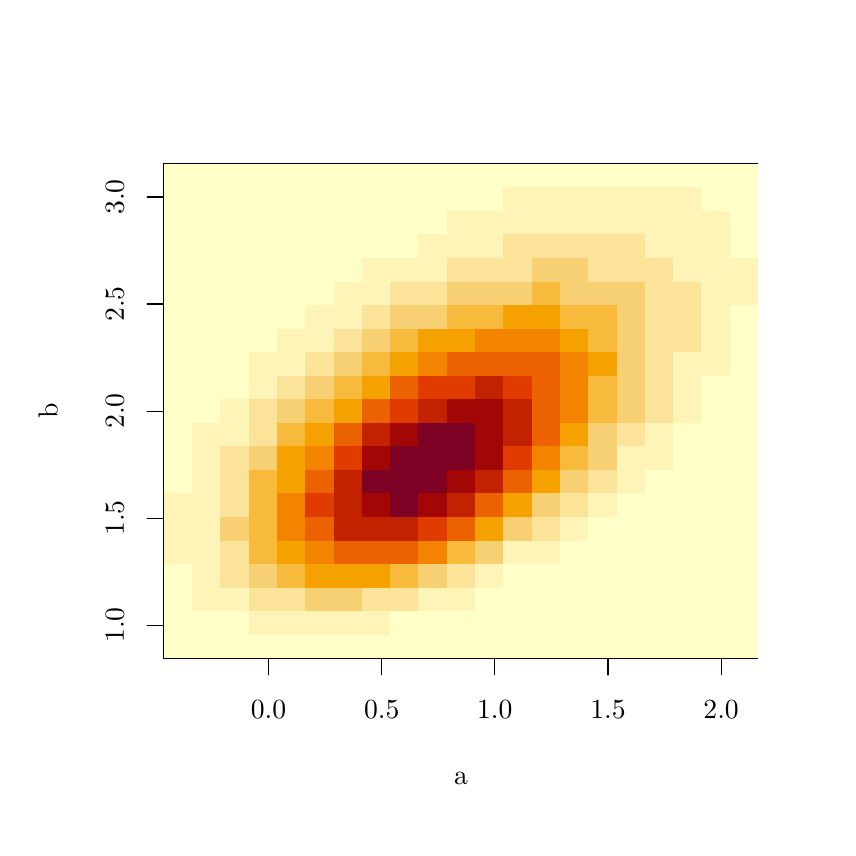
\begin{tikzpicture}[x=1pt,y=1pt]
\definecolor{fillColor}{RGB}{255,255,255}
\path[use as bounding box,fill=fillColor,fill opacity=0.00] (0,0) rectangle (289.08,289.08);
\begin{scope}
\path[clip] (  0.00,  0.00) rectangle (289.08,289.08);
\definecolor{drawColor}{RGB}{0,0,0}

\path[draw=drawColor,line width= 0.4pt,line join=round,line cap=round] ( 87.02, 61.20) -- (250.59, 61.20);

\path[draw=drawColor,line width= 0.4pt,line join=round,line cap=round] ( 87.02, 61.20) -- ( 87.02, 55.20);

\path[draw=drawColor,line width= 0.4pt,line join=round,line cap=round] (127.92, 61.20) -- (127.92, 55.20);

\path[draw=drawColor,line width= 0.4pt,line join=round,line cap=round] (168.81, 61.20) -- (168.81, 55.20);

\path[draw=drawColor,line width= 0.4pt,line join=round,line cap=round] (209.70, 61.20) -- (209.70, 55.20);

\path[draw=drawColor,line width= 0.4pt,line join=round,line cap=round] (250.59, 61.20) -- (250.59, 55.20);

\node[text=drawColor,anchor=base,inner sep=0pt, outer sep=0pt, scale=  1.00] at ( 87.02, 39.60) {0.0};

\node[text=drawColor,anchor=base,inner sep=0pt, outer sep=0pt, scale=  1.00] at (127.92, 39.60) {0.5};

\node[text=drawColor,anchor=base,inner sep=0pt, outer sep=0pt, scale=  1.00] at (168.81, 39.60) {1.0};

\node[text=drawColor,anchor=base,inner sep=0pt, outer sep=0pt, scale=  1.00] at (209.70, 39.60) {1.5};

\node[text=drawColor,anchor=base,inner sep=0pt, outer sep=0pt, scale=  1.00] at (250.59, 39.60) {2.0};

\path[draw=drawColor,line width= 0.4pt,line join=round,line cap=round] ( 49.20, 73.19) -- ( 49.20,227.89);

\path[draw=drawColor,line width= 0.4pt,line join=round,line cap=round] ( 49.20, 73.19) -- ( 43.20, 73.19);

\path[draw=drawColor,line width= 0.4pt,line join=round,line cap=round] ( 49.20,111.86) -- ( 43.20,111.86);

\path[draw=drawColor,line width= 0.4pt,line join=round,line cap=round] ( 49.20,150.54) -- ( 43.20,150.54);

\path[draw=drawColor,line width= 0.4pt,line join=round,line cap=round] ( 49.20,189.22) -- ( 43.20,189.22);

\path[draw=drawColor,line width= 0.4pt,line join=round,line cap=round] ( 49.20,227.89) -- ( 43.20,227.89);

\node[text=drawColor,rotate= 90.00,anchor=base,inner sep=0pt, outer sep=0pt, scale=  1.00] at ( 34.80, 73.19) {1.0};

\node[text=drawColor,rotate= 90.00,anchor=base,inner sep=0pt, outer sep=0pt, scale=  1.00] at ( 34.80,111.86) {1.5};

\node[text=drawColor,rotate= 90.00,anchor=base,inner sep=0pt, outer sep=0pt, scale=  1.00] at ( 34.80,150.54) {2.0};

\node[text=drawColor,rotate= 90.00,anchor=base,inner sep=0pt, outer sep=0pt, scale=  1.00] at ( 34.80,189.22) {2.5};

\node[text=drawColor,rotate= 90.00,anchor=base,inner sep=0pt, outer sep=0pt, scale=  1.00] at ( 34.80,227.89) {3.0};

\path[draw=drawColor,line width= 0.4pt,line join=round,line cap=round] ( 49.20, 61.20) --
	(263.88, 61.20) --
	(263.88,239.88) --
	( 49.20,239.88) --
	( 49.20, 61.20);
\end{scope}
\begin{scope}
\path[clip] (  0.00,  0.00) rectangle (289.08,289.08);
\definecolor{drawColor}{RGB}{0,0,0}

\node[text=drawColor,anchor=base,inner sep=0pt, outer sep=0pt, scale=  1.00] at (156.54, 15.60) {a};

\node[text=drawColor,rotate= 90.00,anchor=base,inner sep=0pt, outer sep=0pt, scale=  1.00] at ( 10.80,150.54) {b};
\end{scope}
\begin{scope}
\path[clip] ( 49.20, 61.20) rectangle (263.88,239.88);
\definecolor{fillColor}{RGB}{255,255,200}

\path[fill=fillColor] ( 49.20, 61.20) rectangle ( 59.42, 69.71);

\path[fill=fillColor] ( 49.20, 69.71) rectangle ( 59.42, 78.22);

\path[fill=fillColor] ( 49.20, 78.22) rectangle ( 59.42, 86.73);

\path[fill=fillColor] ( 49.20, 86.73) rectangle ( 59.42, 95.23);
\definecolor{fillColor}{RGB}{255,244,183}

\path[fill=fillColor] ( 49.20, 95.23) rectangle ( 59.42,103.74);

\path[fill=fillColor] ( 49.20,103.74) rectangle ( 59.42,112.25);

\path[fill=fillColor] ( 49.20,112.25) rectangle ( 59.42,120.76);
\definecolor{fillColor}{RGB}{255,255,200}

\path[fill=fillColor] ( 49.20,120.76) rectangle ( 59.42,129.27);

\path[fill=fillColor] ( 49.20,129.27) rectangle ( 59.42,137.78);

\path[fill=fillColor] ( 49.20,137.78) rectangle ( 59.42,146.29);

\path[fill=fillColor] ( 49.20,146.29) rectangle ( 59.42,154.79);

\path[fill=fillColor] ( 49.20,154.79) rectangle ( 59.42,163.30);

\path[fill=fillColor] ( 49.20,163.30) rectangle ( 59.42,171.81);

\path[fill=fillColor] ( 49.20,171.81) rectangle ( 59.42,180.32);

\path[fill=fillColor] ( 49.20,180.32) rectangle ( 59.42,188.83);

\path[fill=fillColor] ( 49.20,188.83) rectangle ( 59.42,197.34);

\path[fill=fillColor] ( 49.20,197.34) rectangle ( 59.42,205.85);

\path[fill=fillColor] ( 49.20,205.85) rectangle ( 59.42,214.35);

\path[fill=fillColor] ( 49.20,214.35) rectangle ( 59.42,222.86);

\path[fill=fillColor] ( 49.20,222.86) rectangle ( 59.42,231.37);

\path[fill=fillColor] ( 49.20,231.37) rectangle ( 59.42,239.88);

\path[fill=fillColor] ( 59.42, 61.20) rectangle ( 69.65, 69.71);

\path[fill=fillColor] ( 59.42, 69.71) rectangle ( 69.65, 78.22);
\definecolor{fillColor}{RGB}{255,244,183}

\path[fill=fillColor] ( 59.42, 78.22) rectangle ( 69.65, 86.73);

\path[fill=fillColor] ( 59.42, 86.73) rectangle ( 69.65, 95.23);

\path[fill=fillColor] ( 59.42, 95.23) rectangle ( 69.65,103.74);

\path[fill=fillColor] ( 59.42,103.74) rectangle ( 69.65,112.25);

\path[fill=fillColor] ( 59.42,112.25) rectangle ( 69.65,120.76);

\path[fill=fillColor] ( 59.42,120.76) rectangle ( 69.65,129.27);

\path[fill=fillColor] ( 59.42,129.27) rectangle ( 69.65,137.78);

\path[fill=fillColor] ( 59.42,137.78) rectangle ( 69.65,146.29);
\definecolor{fillColor}{RGB}{255,255,200}

\path[fill=fillColor] ( 59.42,146.29) rectangle ( 69.65,154.79);

\path[fill=fillColor] ( 59.42,154.79) rectangle ( 69.65,163.30);

\path[fill=fillColor] ( 59.42,163.30) rectangle ( 69.65,171.81);

\path[fill=fillColor] ( 59.42,171.81) rectangle ( 69.65,180.32);

\path[fill=fillColor] ( 59.42,180.32) rectangle ( 69.65,188.83);

\path[fill=fillColor] ( 59.42,188.83) rectangle ( 69.65,197.34);

\path[fill=fillColor] ( 59.42,197.34) rectangle ( 69.65,205.85);

\path[fill=fillColor] ( 59.42,205.85) rectangle ( 69.65,214.35);

\path[fill=fillColor] ( 59.42,214.35) rectangle ( 69.65,222.86);

\path[fill=fillColor] ( 59.42,222.86) rectangle ( 69.65,231.37);

\path[fill=fillColor] ( 59.42,231.37) rectangle ( 69.65,239.88);

\path[fill=fillColor] ( 69.65, 61.20) rectangle ( 79.87, 69.71);

\path[fill=fillColor] ( 69.65, 69.71) rectangle ( 79.87, 78.22);
\definecolor{fillColor}{RGB}{255,244,183}

\path[fill=fillColor] ( 69.65, 78.22) rectangle ( 79.87, 86.73);
\definecolor{fillColor}{RGB}{251,228,154}

\path[fill=fillColor] ( 69.65, 86.73) rectangle ( 79.87, 95.23);

\path[fill=fillColor] ( 69.65, 95.23) rectangle ( 79.87,103.74);
\definecolor{fillColor}{RGB}{248,208,116}

\path[fill=fillColor] ( 69.65,103.74) rectangle ( 79.87,112.25);
\definecolor{fillColor}{RGB}{251,228,154}

\path[fill=fillColor] ( 69.65,112.25) rectangle ( 79.87,120.76);

\path[fill=fillColor] ( 69.65,120.76) rectangle ( 79.87,129.27);

\path[fill=fillColor] ( 69.65,129.27) rectangle ( 79.87,137.78);
\definecolor{fillColor}{RGB}{255,244,183}

\path[fill=fillColor] ( 69.65,137.78) rectangle ( 79.87,146.29);

\path[fill=fillColor] ( 69.65,146.29) rectangle ( 79.87,154.79);
\definecolor{fillColor}{RGB}{255,255,200}

\path[fill=fillColor] ( 69.65,154.79) rectangle ( 79.87,163.30);

\path[fill=fillColor] ( 69.65,163.30) rectangle ( 79.87,171.81);

\path[fill=fillColor] ( 69.65,171.81) rectangle ( 79.87,180.32);

\path[fill=fillColor] ( 69.65,180.32) rectangle ( 79.87,188.83);

\path[fill=fillColor] ( 69.65,188.83) rectangle ( 79.87,197.34);

\path[fill=fillColor] ( 69.65,197.34) rectangle ( 79.87,205.85);

\path[fill=fillColor] ( 69.65,205.85) rectangle ( 79.87,214.35);

\path[fill=fillColor] ( 69.65,214.35) rectangle ( 79.87,222.86);

\path[fill=fillColor] ( 69.65,222.86) rectangle ( 79.87,231.37);

\path[fill=fillColor] ( 69.65,231.37) rectangle ( 79.87,239.88);

\path[fill=fillColor] ( 79.87, 61.20) rectangle ( 90.09, 69.71);
\definecolor{fillColor}{RGB}{255,244,183}

\path[fill=fillColor] ( 79.87, 69.71) rectangle ( 90.09, 78.22);
\definecolor{fillColor}{RGB}{251,228,154}

\path[fill=fillColor] ( 79.87, 78.22) rectangle ( 90.09, 86.73);
\definecolor{fillColor}{RGB}{248,208,116}

\path[fill=fillColor] ( 79.87, 86.73) rectangle ( 90.09, 95.23);
\definecolor{fillColor}{RGB}{247,186,60}

\path[fill=fillColor] ( 79.87, 95.23) rectangle ( 90.09,103.74);

\path[fill=fillColor] ( 79.87,103.74) rectangle ( 90.09,112.25);

\path[fill=fillColor] ( 79.87,112.25) rectangle ( 90.09,120.76);

\path[fill=fillColor] ( 79.87,120.76) rectangle ( 90.09,129.27);
\definecolor{fillColor}{RGB}{248,208,116}

\path[fill=fillColor] ( 79.87,129.27) rectangle ( 90.09,137.78);
\definecolor{fillColor}{RGB}{251,228,154}

\path[fill=fillColor] ( 79.87,137.78) rectangle ( 90.09,146.29);

\path[fill=fillColor] ( 79.87,146.29) rectangle ( 90.09,154.79);
\definecolor{fillColor}{RGB}{255,244,183}

\path[fill=fillColor] ( 79.87,154.79) rectangle ( 90.09,163.30);

\path[fill=fillColor] ( 79.87,163.30) rectangle ( 90.09,171.81);
\definecolor{fillColor}{RGB}{255,255,200}

\path[fill=fillColor] ( 79.87,171.81) rectangle ( 90.09,180.32);

\path[fill=fillColor] ( 79.87,180.32) rectangle ( 90.09,188.83);

\path[fill=fillColor] ( 79.87,188.83) rectangle ( 90.09,197.34);

\path[fill=fillColor] ( 79.87,197.34) rectangle ( 90.09,205.85);

\path[fill=fillColor] ( 79.87,205.85) rectangle ( 90.09,214.35);

\path[fill=fillColor] ( 79.87,214.35) rectangle ( 90.09,222.86);

\path[fill=fillColor] ( 79.87,222.86) rectangle ( 90.09,231.37);

\path[fill=fillColor] ( 79.87,231.37) rectangle ( 90.09,239.88);

\path[fill=fillColor] ( 90.09, 61.20) rectangle (100.31, 69.71);
\definecolor{fillColor}{RGB}{255,244,183}

\path[fill=fillColor] ( 90.09, 69.71) rectangle (100.31, 78.22);
\definecolor{fillColor}{RGB}{251,228,154}

\path[fill=fillColor] ( 90.09, 78.22) rectangle (100.31, 86.73);
\definecolor{fillColor}{RGB}{247,186,60}

\path[fill=fillColor] ( 90.09, 86.73) rectangle (100.31, 95.23);
\definecolor{fillColor}{RGB}{245,161,0}

\path[fill=fillColor] ( 90.09, 95.23) rectangle (100.31,103.74);
\definecolor{fillColor}{RGB}{242,132,0}

\path[fill=fillColor] ( 90.09,103.74) rectangle (100.31,112.25);

\path[fill=fillColor] ( 90.09,112.25) rectangle (100.31,120.76);
\definecolor{fillColor}{RGB}{245,161,0}

\path[fill=fillColor] ( 90.09,120.76) rectangle (100.31,129.27);

\path[fill=fillColor] ( 90.09,129.27) rectangle (100.31,137.78);
\definecolor{fillColor}{RGB}{247,186,60}

\path[fill=fillColor] ( 90.09,137.78) rectangle (100.31,146.29);
\definecolor{fillColor}{RGB}{248,208,116}

\path[fill=fillColor] ( 90.09,146.29) rectangle (100.31,154.79);
\definecolor{fillColor}{RGB}{251,228,154}

\path[fill=fillColor] ( 90.09,154.79) rectangle (100.31,163.30);
\definecolor{fillColor}{RGB}{255,244,183}

\path[fill=fillColor] ( 90.09,163.30) rectangle (100.31,171.81);

\path[fill=fillColor] ( 90.09,171.81) rectangle (100.31,180.32);
\definecolor{fillColor}{RGB}{255,255,200}

\path[fill=fillColor] ( 90.09,180.32) rectangle (100.31,188.83);

\path[fill=fillColor] ( 90.09,188.83) rectangle (100.31,197.34);

\path[fill=fillColor] ( 90.09,197.34) rectangle (100.31,205.85);

\path[fill=fillColor] ( 90.09,205.85) rectangle (100.31,214.35);

\path[fill=fillColor] ( 90.09,214.35) rectangle (100.31,222.86);

\path[fill=fillColor] ( 90.09,222.86) rectangle (100.31,231.37);

\path[fill=fillColor] ( 90.09,231.37) rectangle (100.31,239.88);

\path[fill=fillColor] (100.31, 61.20) rectangle (110.54, 69.71);
\definecolor{fillColor}{RGB}{255,244,183}

\path[fill=fillColor] (100.31, 69.71) rectangle (110.54, 78.22);
\definecolor{fillColor}{RGB}{248,208,116}

\path[fill=fillColor] (100.31, 78.22) rectangle (110.54, 86.73);
\definecolor{fillColor}{RGB}{245,161,0}

\path[fill=fillColor] (100.31, 86.73) rectangle (110.54, 95.23);
\definecolor{fillColor}{RGB}{242,132,0}

\path[fill=fillColor] (100.31, 95.23) rectangle (110.54,103.74);
\definecolor{fillColor}{RGB}{237,98,0}

\path[fill=fillColor] (100.31,103.74) rectangle (110.54,112.25);
\definecolor{fillColor}{RGB}{225,60,0}

\path[fill=fillColor] (100.31,112.25) rectangle (110.54,120.76);
\definecolor{fillColor}{RGB}{237,98,0}

\path[fill=fillColor] (100.31,120.76) rectangle (110.54,129.27);
\definecolor{fillColor}{RGB}{242,132,0}

\path[fill=fillColor] (100.31,129.27) rectangle (110.54,137.78);
\definecolor{fillColor}{RGB}{245,161,0}

\path[fill=fillColor] (100.31,137.78) rectangle (110.54,146.29);
\definecolor{fillColor}{RGB}{247,186,60}

\path[fill=fillColor] (100.31,146.29) rectangle (110.54,154.79);
\definecolor{fillColor}{RGB}{248,208,116}

\path[fill=fillColor] (100.31,154.79) rectangle (110.54,163.30);
\definecolor{fillColor}{RGB}{251,228,154}

\path[fill=fillColor] (100.31,163.30) rectangle (110.54,171.81);
\definecolor{fillColor}{RGB}{255,244,183}

\path[fill=fillColor] (100.31,171.81) rectangle (110.54,180.32);

\path[fill=fillColor] (100.31,180.32) rectangle (110.54,188.83);
\definecolor{fillColor}{RGB}{255,255,200}

\path[fill=fillColor] (100.31,188.83) rectangle (110.54,197.34);

\path[fill=fillColor] (100.31,197.34) rectangle (110.54,205.85);

\path[fill=fillColor] (100.31,205.85) rectangle (110.54,214.35);

\path[fill=fillColor] (100.31,214.35) rectangle (110.54,222.86);

\path[fill=fillColor] (100.31,222.86) rectangle (110.54,231.37);

\path[fill=fillColor] (100.31,231.37) rectangle (110.54,239.88);

\path[fill=fillColor] (110.54, 61.20) rectangle (120.76, 69.71);
\definecolor{fillColor}{RGB}{255,244,183}

\path[fill=fillColor] (110.54, 69.71) rectangle (120.76, 78.22);
\definecolor{fillColor}{RGB}{248,208,116}

\path[fill=fillColor] (110.54, 78.22) rectangle (120.76, 86.73);
\definecolor{fillColor}{RGB}{245,161,0}

\path[fill=fillColor] (110.54, 86.73) rectangle (120.76, 95.23);
\definecolor{fillColor}{RGB}{237,98,0}

\path[fill=fillColor] (110.54, 95.23) rectangle (120.76,103.74);
\definecolor{fillColor}{RGB}{195,34,0}

\path[fill=fillColor] (110.54,103.74) rectangle (120.76,112.25);

\path[fill=fillColor] (110.54,112.25) rectangle (120.76,120.76);

\path[fill=fillColor] (110.54,120.76) rectangle (120.76,129.27);
\definecolor{fillColor}{RGB}{225,60,0}

\path[fill=fillColor] (110.54,129.27) rectangle (120.76,137.78);
\definecolor{fillColor}{RGB}{237,98,0}

\path[fill=fillColor] (110.54,137.78) rectangle (120.76,146.29);
\definecolor{fillColor}{RGB}{245,161,0}

\path[fill=fillColor] (110.54,146.29) rectangle (120.76,154.79);
\definecolor{fillColor}{RGB}{247,186,60}

\path[fill=fillColor] (110.54,154.79) rectangle (120.76,163.30);
\definecolor{fillColor}{RGB}{248,208,116}

\path[fill=fillColor] (110.54,163.30) rectangle (120.76,171.81);
\definecolor{fillColor}{RGB}{251,228,154}

\path[fill=fillColor] (110.54,171.81) rectangle (120.76,180.32);
\definecolor{fillColor}{RGB}{255,244,183}

\path[fill=fillColor] (110.54,180.32) rectangle (120.76,188.83);

\path[fill=fillColor] (110.54,188.83) rectangle (120.76,197.34);
\definecolor{fillColor}{RGB}{255,255,200}

\path[fill=fillColor] (110.54,197.34) rectangle (120.76,205.85);

\path[fill=fillColor] (110.54,205.85) rectangle (120.76,214.35);

\path[fill=fillColor] (110.54,214.35) rectangle (120.76,222.86);

\path[fill=fillColor] (110.54,222.86) rectangle (120.76,231.37);

\path[fill=fillColor] (110.54,231.37) rectangle (120.76,239.88);

\path[fill=fillColor] (120.76, 61.20) rectangle (130.98, 69.71);
\definecolor{fillColor}{RGB}{255,244,183}

\path[fill=fillColor] (120.76, 69.71) rectangle (130.98, 78.22);
\definecolor{fillColor}{RGB}{251,228,154}

\path[fill=fillColor] (120.76, 78.22) rectangle (130.98, 86.73);
\definecolor{fillColor}{RGB}{245,161,0}

\path[fill=fillColor] (120.76, 86.73) rectangle (130.98, 95.23);
\definecolor{fillColor}{RGB}{237,98,0}

\path[fill=fillColor] (120.76, 95.23) rectangle (130.98,103.74);
\definecolor{fillColor}{RGB}{195,34,0}

\path[fill=fillColor] (120.76,103.74) rectangle (130.98,112.25);
\definecolor{fillColor}{RGB}{162,7,6}

\path[fill=fillColor] (120.76,112.25) rectangle (130.98,120.76);
\definecolor{fillColor}{RGB}{125,0,37}

\path[fill=fillColor] (120.76,120.76) rectangle (130.98,129.27);
\definecolor{fillColor}{RGB}{162,7,6}

\path[fill=fillColor] (120.76,129.27) rectangle (130.98,137.78);
\definecolor{fillColor}{RGB}{195,34,0}

\path[fill=fillColor] (120.76,137.78) rectangle (130.98,146.29);
\definecolor{fillColor}{RGB}{237,98,0}

\path[fill=fillColor] (120.76,146.29) rectangle (130.98,154.79);
\definecolor{fillColor}{RGB}{245,161,0}

\path[fill=fillColor] (120.76,154.79) rectangle (130.98,163.30);
\definecolor{fillColor}{RGB}{247,186,60}

\path[fill=fillColor] (120.76,163.30) rectangle (130.98,171.81);
\definecolor{fillColor}{RGB}{248,208,116}

\path[fill=fillColor] (120.76,171.81) rectangle (130.98,180.32);
\definecolor{fillColor}{RGB}{251,228,154}

\path[fill=fillColor] (120.76,180.32) rectangle (130.98,188.83);
\definecolor{fillColor}{RGB}{255,244,183}

\path[fill=fillColor] (120.76,188.83) rectangle (130.98,197.34);

\path[fill=fillColor] (120.76,197.34) rectangle (130.98,205.85);
\definecolor{fillColor}{RGB}{255,255,200}

\path[fill=fillColor] (120.76,205.85) rectangle (130.98,214.35);

\path[fill=fillColor] (120.76,214.35) rectangle (130.98,222.86);

\path[fill=fillColor] (120.76,222.86) rectangle (130.98,231.37);

\path[fill=fillColor] (120.76,231.37) rectangle (130.98,239.88);

\path[fill=fillColor] (130.98, 61.20) rectangle (141.21, 69.71);

\path[fill=fillColor] (130.98, 69.71) rectangle (141.21, 78.22);
\definecolor{fillColor}{RGB}{251,228,154}

\path[fill=fillColor] (130.98, 78.22) rectangle (141.21, 86.73);
\definecolor{fillColor}{RGB}{247,186,60}

\path[fill=fillColor] (130.98, 86.73) rectangle (141.21, 95.23);
\definecolor{fillColor}{RGB}{237,98,0}

\path[fill=fillColor] (130.98, 95.23) rectangle (141.21,103.74);
\definecolor{fillColor}{RGB}{195,34,0}

\path[fill=fillColor] (130.98,103.74) rectangle (141.21,112.25);
\definecolor{fillColor}{RGB}{125,0,37}

\path[fill=fillColor] (130.98,112.25) rectangle (141.21,120.76);

\path[fill=fillColor] (130.98,120.76) rectangle (141.21,129.27);

\path[fill=fillColor] (130.98,129.27) rectangle (141.21,137.78);
\definecolor{fillColor}{RGB}{162,7,6}

\path[fill=fillColor] (130.98,137.78) rectangle (141.21,146.29);
\definecolor{fillColor}{RGB}{225,60,0}

\path[fill=fillColor] (130.98,146.29) rectangle (141.21,154.79);
\definecolor{fillColor}{RGB}{237,98,0}

\path[fill=fillColor] (130.98,154.79) rectangle (141.21,163.30);
\definecolor{fillColor}{RGB}{245,161,0}

\path[fill=fillColor] (130.98,163.30) rectangle (141.21,171.81);
\definecolor{fillColor}{RGB}{247,186,60}

\path[fill=fillColor] (130.98,171.81) rectangle (141.21,180.32);
\definecolor{fillColor}{RGB}{248,208,116}

\path[fill=fillColor] (130.98,180.32) rectangle (141.21,188.83);
\definecolor{fillColor}{RGB}{251,228,154}

\path[fill=fillColor] (130.98,188.83) rectangle (141.21,197.34);
\definecolor{fillColor}{RGB}{255,244,183}

\path[fill=fillColor] (130.98,197.34) rectangle (141.21,205.85);
\definecolor{fillColor}{RGB}{255,255,200}

\path[fill=fillColor] (130.98,205.85) rectangle (141.21,214.35);

\path[fill=fillColor] (130.98,214.35) rectangle (141.21,222.86);

\path[fill=fillColor] (130.98,222.86) rectangle (141.21,231.37);

\path[fill=fillColor] (130.98,231.37) rectangle (141.21,239.88);

\path[fill=fillColor] (141.21, 61.20) rectangle (151.43, 69.71);

\path[fill=fillColor] (141.21, 69.71) rectangle (151.43, 78.22);
\definecolor{fillColor}{RGB}{255,244,183}

\path[fill=fillColor] (141.21, 78.22) rectangle (151.43, 86.73);
\definecolor{fillColor}{RGB}{248,208,116}

\path[fill=fillColor] (141.21, 86.73) rectangle (151.43, 95.23);
\definecolor{fillColor}{RGB}{242,132,0}

\path[fill=fillColor] (141.21, 95.23) rectangle (151.43,103.74);
\definecolor{fillColor}{RGB}{225,60,0}

\path[fill=fillColor] (141.21,103.74) rectangle (151.43,112.25);
\definecolor{fillColor}{RGB}{162,7,6}

\path[fill=fillColor] (141.21,112.25) rectangle (151.43,120.76);
\definecolor{fillColor}{RGB}{125,0,37}

\path[fill=fillColor] (141.21,120.76) rectangle (151.43,129.27);

\path[fill=fillColor] (141.21,129.27) rectangle (151.43,137.78);

\path[fill=fillColor] (141.21,137.78) rectangle (151.43,146.29);
\definecolor{fillColor}{RGB}{195,34,0}

\path[fill=fillColor] (141.21,146.29) rectangle (151.43,154.79);
\definecolor{fillColor}{RGB}{225,60,0}

\path[fill=fillColor] (141.21,154.79) rectangle (151.43,163.30);
\definecolor{fillColor}{RGB}{242,132,0}

\path[fill=fillColor] (141.21,163.30) rectangle (151.43,171.81);
\definecolor{fillColor}{RGB}{245,161,0}

\path[fill=fillColor] (141.21,171.81) rectangle (151.43,180.32);
\definecolor{fillColor}{RGB}{248,208,116}

\path[fill=fillColor] (141.21,180.32) rectangle (151.43,188.83);
\definecolor{fillColor}{RGB}{251,228,154}

\path[fill=fillColor] (141.21,188.83) rectangle (151.43,197.34);
\definecolor{fillColor}{RGB}{255,244,183}

\path[fill=fillColor] (141.21,197.34) rectangle (151.43,205.85);

\path[fill=fillColor] (141.21,205.85) rectangle (151.43,214.35);
\definecolor{fillColor}{RGB}{255,255,200}

\path[fill=fillColor] (141.21,214.35) rectangle (151.43,222.86);

\path[fill=fillColor] (141.21,222.86) rectangle (151.43,231.37);

\path[fill=fillColor] (141.21,231.37) rectangle (151.43,239.88);

\path[fill=fillColor] (151.43, 61.20) rectangle (161.65, 69.71);

\path[fill=fillColor] (151.43, 69.71) rectangle (161.65, 78.22);
\definecolor{fillColor}{RGB}{255,244,183}

\path[fill=fillColor] (151.43, 78.22) rectangle (161.65, 86.73);
\definecolor{fillColor}{RGB}{251,228,154}

\path[fill=fillColor] (151.43, 86.73) rectangle (161.65, 95.23);
\definecolor{fillColor}{RGB}{247,186,60}

\path[fill=fillColor] (151.43, 95.23) rectangle (161.65,103.74);
\definecolor{fillColor}{RGB}{237,98,0}

\path[fill=fillColor] (151.43,103.74) rectangle (161.65,112.25);
\definecolor{fillColor}{RGB}{195,34,0}

\path[fill=fillColor] (151.43,112.25) rectangle (161.65,120.76);
\definecolor{fillColor}{RGB}{162,7,6}

\path[fill=fillColor] (151.43,120.76) rectangle (161.65,129.27);
\definecolor{fillColor}{RGB}{125,0,37}

\path[fill=fillColor] (151.43,129.27) rectangle (161.65,137.78);

\path[fill=fillColor] (151.43,137.78) rectangle (161.65,146.29);
\definecolor{fillColor}{RGB}{162,7,6}

\path[fill=fillColor] (151.43,146.29) rectangle (161.65,154.79);
\definecolor{fillColor}{RGB}{225,60,0}

\path[fill=fillColor] (151.43,154.79) rectangle (161.65,163.30);
\definecolor{fillColor}{RGB}{237,98,0}

\path[fill=fillColor] (151.43,163.30) rectangle (161.65,171.81);
\definecolor{fillColor}{RGB}{245,161,0}

\path[fill=fillColor] (151.43,171.81) rectangle (161.65,180.32);
\definecolor{fillColor}{RGB}{247,186,60}

\path[fill=fillColor] (151.43,180.32) rectangle (161.65,188.83);
\definecolor{fillColor}{RGB}{248,208,116}

\path[fill=fillColor] (151.43,188.83) rectangle (161.65,197.34);
\definecolor{fillColor}{RGB}{251,228,154}

\path[fill=fillColor] (151.43,197.34) rectangle (161.65,205.85);
\definecolor{fillColor}{RGB}{255,244,183}

\path[fill=fillColor] (151.43,205.85) rectangle (161.65,214.35);

\path[fill=fillColor] (151.43,214.35) rectangle (161.65,222.86);
\definecolor{fillColor}{RGB}{255,255,200}

\path[fill=fillColor] (151.43,222.86) rectangle (161.65,231.37);

\path[fill=fillColor] (151.43,231.37) rectangle (161.65,239.88);

\path[fill=fillColor] (161.65, 61.20) rectangle (171.87, 69.71);

\path[fill=fillColor] (161.65, 69.71) rectangle (171.87, 78.22);

\path[fill=fillColor] (161.65, 78.22) rectangle (171.87, 86.73);
\definecolor{fillColor}{RGB}{255,244,183}

\path[fill=fillColor] (161.65, 86.73) rectangle (171.87, 95.23);
\definecolor{fillColor}{RGB}{248,208,116}

\path[fill=fillColor] (161.65, 95.23) rectangle (171.87,103.74);
\definecolor{fillColor}{RGB}{245,161,0}

\path[fill=fillColor] (161.65,103.74) rectangle (171.87,112.25);
\definecolor{fillColor}{RGB}{237,98,0}

\path[fill=fillColor] (161.65,112.25) rectangle (171.87,120.76);
\definecolor{fillColor}{RGB}{195,34,0}

\path[fill=fillColor] (161.65,120.76) rectangle (171.87,129.27);
\definecolor{fillColor}{RGB}{162,7,6}

\path[fill=fillColor] (161.65,129.27) rectangle (171.87,137.78);

\path[fill=fillColor] (161.65,137.78) rectangle (171.87,146.29);

\path[fill=fillColor] (161.65,146.29) rectangle (171.87,154.79);
\definecolor{fillColor}{RGB}{195,34,0}

\path[fill=fillColor] (161.65,154.79) rectangle (171.87,163.30);
\definecolor{fillColor}{RGB}{237,98,0}

\path[fill=fillColor] (161.65,163.30) rectangle (171.87,171.81);
\definecolor{fillColor}{RGB}{242,132,0}

\path[fill=fillColor] (161.65,171.81) rectangle (171.87,180.32);
\definecolor{fillColor}{RGB}{247,186,60}

\path[fill=fillColor] (161.65,180.32) rectangle (171.87,188.83);
\definecolor{fillColor}{RGB}{248,208,116}

\path[fill=fillColor] (161.65,188.83) rectangle (171.87,197.34);
\definecolor{fillColor}{RGB}{251,228,154}

\path[fill=fillColor] (161.65,197.34) rectangle (171.87,205.85);
\definecolor{fillColor}{RGB}{255,244,183}

\path[fill=fillColor] (161.65,205.85) rectangle (171.87,214.35);

\path[fill=fillColor] (161.65,214.35) rectangle (171.87,222.86);
\definecolor{fillColor}{RGB}{255,255,200}

\path[fill=fillColor] (161.65,222.86) rectangle (171.87,231.37);

\path[fill=fillColor] (161.65,231.37) rectangle (171.87,239.88);

\path[fill=fillColor] (171.87, 61.20) rectangle (182.10, 69.71);

\path[fill=fillColor] (171.87, 69.71) rectangle (182.10, 78.22);

\path[fill=fillColor] (171.87, 78.22) rectangle (182.10, 86.73);

\path[fill=fillColor] (171.87, 86.73) rectangle (182.10, 95.23);
\definecolor{fillColor}{RGB}{255,244,183}

\path[fill=fillColor] (171.87, 95.23) rectangle (182.10,103.74);
\definecolor{fillColor}{RGB}{248,208,116}

\path[fill=fillColor] (171.87,103.74) rectangle (182.10,112.25);
\definecolor{fillColor}{RGB}{245,161,0}

\path[fill=fillColor] (171.87,112.25) rectangle (182.10,120.76);
\definecolor{fillColor}{RGB}{237,98,0}

\path[fill=fillColor] (171.87,120.76) rectangle (182.10,129.27);
\definecolor{fillColor}{RGB}{225,60,0}

\path[fill=fillColor] (171.87,129.27) rectangle (182.10,137.78);
\definecolor{fillColor}{RGB}{195,34,0}

\path[fill=fillColor] (171.87,137.78) rectangle (182.10,146.29);

\path[fill=fillColor] (171.87,146.29) rectangle (182.10,154.79);
\definecolor{fillColor}{RGB}{225,60,0}

\path[fill=fillColor] (171.87,154.79) rectangle (182.10,163.30);
\definecolor{fillColor}{RGB}{237,98,0}

\path[fill=fillColor] (171.87,163.30) rectangle (182.10,171.81);
\definecolor{fillColor}{RGB}{242,132,0}

\path[fill=fillColor] (171.87,171.81) rectangle (182.10,180.32);
\definecolor{fillColor}{RGB}{245,161,0}

\path[fill=fillColor] (171.87,180.32) rectangle (182.10,188.83);
\definecolor{fillColor}{RGB}{248,208,116}

\path[fill=fillColor] (171.87,188.83) rectangle (182.10,197.34);
\definecolor{fillColor}{RGB}{251,228,154}

\path[fill=fillColor] (171.87,197.34) rectangle (182.10,205.85);

\path[fill=fillColor] (171.87,205.85) rectangle (182.10,214.35);
\definecolor{fillColor}{RGB}{255,244,183}

\path[fill=fillColor] (171.87,214.35) rectangle (182.10,222.86);

\path[fill=fillColor] (171.87,222.86) rectangle (182.10,231.37);
\definecolor{fillColor}{RGB}{255,255,200}

\path[fill=fillColor] (171.87,231.37) rectangle (182.10,239.88);

\path[fill=fillColor] (182.10, 61.20) rectangle (192.32, 69.71);

\path[fill=fillColor] (182.10, 69.71) rectangle (192.32, 78.22);

\path[fill=fillColor] (182.10, 78.22) rectangle (192.32, 86.73);

\path[fill=fillColor] (182.10, 86.73) rectangle (192.32, 95.23);
\definecolor{fillColor}{RGB}{255,244,183}

\path[fill=fillColor] (182.10, 95.23) rectangle (192.32,103.74);
\definecolor{fillColor}{RGB}{251,228,154}

\path[fill=fillColor] (182.10,103.74) rectangle (192.32,112.25);
\definecolor{fillColor}{RGB}{248,208,116}

\path[fill=fillColor] (182.10,112.25) rectangle (192.32,120.76);
\definecolor{fillColor}{RGB}{245,161,0}

\path[fill=fillColor] (182.10,120.76) rectangle (192.32,129.27);
\definecolor{fillColor}{RGB}{242,132,0}

\path[fill=fillColor] (182.10,129.27) rectangle (192.32,137.78);
\definecolor{fillColor}{RGB}{237,98,0}

\path[fill=fillColor] (182.10,137.78) rectangle (192.32,146.29);

\path[fill=fillColor] (182.10,146.29) rectangle (192.32,154.79);

\path[fill=fillColor] (182.10,154.79) rectangle (192.32,163.30);

\path[fill=fillColor] (182.10,163.30) rectangle (192.32,171.81);
\definecolor{fillColor}{RGB}{242,132,0}

\path[fill=fillColor] (182.10,171.81) rectangle (192.32,180.32);
\definecolor{fillColor}{RGB}{245,161,0}

\path[fill=fillColor] (182.10,180.32) rectangle (192.32,188.83);
\definecolor{fillColor}{RGB}{247,186,60}

\path[fill=fillColor] (182.10,188.83) rectangle (192.32,197.34);
\definecolor{fillColor}{RGB}{248,208,116}

\path[fill=fillColor] (182.10,197.34) rectangle (192.32,205.85);
\definecolor{fillColor}{RGB}{251,228,154}

\path[fill=fillColor] (182.10,205.85) rectangle (192.32,214.35);
\definecolor{fillColor}{RGB}{255,244,183}

\path[fill=fillColor] (182.10,214.35) rectangle (192.32,222.86);

\path[fill=fillColor] (182.10,222.86) rectangle (192.32,231.37);
\definecolor{fillColor}{RGB}{255,255,200}

\path[fill=fillColor] (182.10,231.37) rectangle (192.32,239.88);

\path[fill=fillColor] (192.32, 61.20) rectangle (202.54, 69.71);

\path[fill=fillColor] (192.32, 69.71) rectangle (202.54, 78.22);

\path[fill=fillColor] (192.32, 78.22) rectangle (202.54, 86.73);

\path[fill=fillColor] (192.32, 86.73) rectangle (202.54, 95.23);

\path[fill=fillColor] (192.32, 95.23) rectangle (202.54,103.74);
\definecolor{fillColor}{RGB}{255,244,183}

\path[fill=fillColor] (192.32,103.74) rectangle (202.54,112.25);
\definecolor{fillColor}{RGB}{251,228,154}

\path[fill=fillColor] (192.32,112.25) rectangle (202.54,120.76);
\definecolor{fillColor}{RGB}{248,208,116}

\path[fill=fillColor] (192.32,120.76) rectangle (202.54,129.27);
\definecolor{fillColor}{RGB}{247,186,60}

\path[fill=fillColor] (192.32,129.27) rectangle (202.54,137.78);
\definecolor{fillColor}{RGB}{245,161,0}

\path[fill=fillColor] (192.32,137.78) rectangle (202.54,146.29);
\definecolor{fillColor}{RGB}{242,132,0}

\path[fill=fillColor] (192.32,146.29) rectangle (202.54,154.79);

\path[fill=fillColor] (192.32,154.79) rectangle (202.54,163.30);

\path[fill=fillColor] (192.32,163.30) rectangle (202.54,171.81);
\definecolor{fillColor}{RGB}{245,161,0}

\path[fill=fillColor] (192.32,171.81) rectangle (202.54,180.32);
\definecolor{fillColor}{RGB}{247,186,60}

\path[fill=fillColor] (192.32,180.32) rectangle (202.54,188.83);
\definecolor{fillColor}{RGB}{248,208,116}

\path[fill=fillColor] (192.32,188.83) rectangle (202.54,197.34);

\path[fill=fillColor] (192.32,197.34) rectangle (202.54,205.85);
\definecolor{fillColor}{RGB}{251,228,154}

\path[fill=fillColor] (192.32,205.85) rectangle (202.54,214.35);
\definecolor{fillColor}{RGB}{255,244,183}

\path[fill=fillColor] (192.32,214.35) rectangle (202.54,222.86);

\path[fill=fillColor] (192.32,222.86) rectangle (202.54,231.37);
\definecolor{fillColor}{RGB}{255,255,200}

\path[fill=fillColor] (192.32,231.37) rectangle (202.54,239.88);

\path[fill=fillColor] (202.54, 61.20) rectangle (212.77, 69.71);

\path[fill=fillColor] (202.54, 69.71) rectangle (212.77, 78.22);

\path[fill=fillColor] (202.54, 78.22) rectangle (212.77, 86.73);

\path[fill=fillColor] (202.54, 86.73) rectangle (212.77, 95.23);

\path[fill=fillColor] (202.54, 95.23) rectangle (212.77,103.74);

\path[fill=fillColor] (202.54,103.74) rectangle (212.77,112.25);
\definecolor{fillColor}{RGB}{255,244,183}

\path[fill=fillColor] (202.54,112.25) rectangle (212.77,120.76);
\definecolor{fillColor}{RGB}{251,228,154}

\path[fill=fillColor] (202.54,120.76) rectangle (212.77,129.27);
\definecolor{fillColor}{RGB}{248,208,116}

\path[fill=fillColor] (202.54,129.27) rectangle (212.77,137.78);

\path[fill=fillColor] (202.54,137.78) rectangle (212.77,146.29);
\definecolor{fillColor}{RGB}{247,186,60}

\path[fill=fillColor] (202.54,146.29) rectangle (212.77,154.79);

\path[fill=fillColor] (202.54,154.79) rectangle (212.77,163.30);
\definecolor{fillColor}{RGB}{245,161,0}

\path[fill=fillColor] (202.54,163.30) rectangle (212.77,171.81);
\definecolor{fillColor}{RGB}{247,186,60}

\path[fill=fillColor] (202.54,171.81) rectangle (212.77,180.32);

\path[fill=fillColor] (202.54,180.32) rectangle (212.77,188.83);
\definecolor{fillColor}{RGB}{248,208,116}

\path[fill=fillColor] (202.54,188.83) rectangle (212.77,197.34);
\definecolor{fillColor}{RGB}{251,228,154}

\path[fill=fillColor] (202.54,197.34) rectangle (212.77,205.85);

\path[fill=fillColor] (202.54,205.85) rectangle (212.77,214.35);
\definecolor{fillColor}{RGB}{255,244,183}

\path[fill=fillColor] (202.54,214.35) rectangle (212.77,222.86);

\path[fill=fillColor] (202.54,222.86) rectangle (212.77,231.37);
\definecolor{fillColor}{RGB}{255,255,200}

\path[fill=fillColor] (202.54,231.37) rectangle (212.77,239.88);

\path[fill=fillColor] (212.77, 61.20) rectangle (222.99, 69.71);

\path[fill=fillColor] (212.77, 69.71) rectangle (222.99, 78.22);

\path[fill=fillColor] (212.77, 78.22) rectangle (222.99, 86.73);

\path[fill=fillColor] (212.77, 86.73) rectangle (222.99, 95.23);

\path[fill=fillColor] (212.77, 95.23) rectangle (222.99,103.74);

\path[fill=fillColor] (212.77,103.74) rectangle (222.99,112.25);

\path[fill=fillColor] (212.77,112.25) rectangle (222.99,120.76);
\definecolor{fillColor}{RGB}{255,244,183}

\path[fill=fillColor] (212.77,120.76) rectangle (222.99,129.27);

\path[fill=fillColor] (212.77,129.27) rectangle (222.99,137.78);
\definecolor{fillColor}{RGB}{251,228,154}

\path[fill=fillColor] (212.77,137.78) rectangle (222.99,146.29);
\definecolor{fillColor}{RGB}{248,208,116}

\path[fill=fillColor] (212.77,146.29) rectangle (222.99,154.79);

\path[fill=fillColor] (212.77,154.79) rectangle (222.99,163.30);

\path[fill=fillColor] (212.77,163.30) rectangle (222.99,171.81);

\path[fill=fillColor] (212.77,171.81) rectangle (222.99,180.32);

\path[fill=fillColor] (212.77,180.32) rectangle (222.99,188.83);

\path[fill=fillColor] (212.77,188.83) rectangle (222.99,197.34);
\definecolor{fillColor}{RGB}{251,228,154}

\path[fill=fillColor] (212.77,197.34) rectangle (222.99,205.85);

\path[fill=fillColor] (212.77,205.85) rectangle (222.99,214.35);
\definecolor{fillColor}{RGB}{255,244,183}

\path[fill=fillColor] (212.77,214.35) rectangle (222.99,222.86);

\path[fill=fillColor] (212.77,222.86) rectangle (222.99,231.37);
\definecolor{fillColor}{RGB}{255,255,200}

\path[fill=fillColor] (212.77,231.37) rectangle (222.99,239.88);

\path[fill=fillColor] (222.99, 61.20) rectangle (233.21, 69.71);

\path[fill=fillColor] (222.99, 69.71) rectangle (233.21, 78.22);

\path[fill=fillColor] (222.99, 78.22) rectangle (233.21, 86.73);

\path[fill=fillColor] (222.99, 86.73) rectangle (233.21, 95.23);

\path[fill=fillColor] (222.99, 95.23) rectangle (233.21,103.74);

\path[fill=fillColor] (222.99,103.74) rectangle (233.21,112.25);

\path[fill=fillColor] (222.99,112.25) rectangle (233.21,120.76);

\path[fill=fillColor] (222.99,120.76) rectangle (233.21,129.27);
\definecolor{fillColor}{RGB}{255,244,183}

\path[fill=fillColor] (222.99,129.27) rectangle (233.21,137.78);

\path[fill=fillColor] (222.99,137.78) rectangle (233.21,146.29);
\definecolor{fillColor}{RGB}{251,228,154}

\path[fill=fillColor] (222.99,146.29) rectangle (233.21,154.79);

\path[fill=fillColor] (222.99,154.79) rectangle (233.21,163.30);

\path[fill=fillColor] (222.99,163.30) rectangle (233.21,171.81);

\path[fill=fillColor] (222.99,171.81) rectangle (233.21,180.32);

\path[fill=fillColor] (222.99,180.32) rectangle (233.21,188.83);

\path[fill=fillColor] (222.99,188.83) rectangle (233.21,197.34);

\path[fill=fillColor] (222.99,197.34) rectangle (233.21,205.85);
\definecolor{fillColor}{RGB}{255,244,183}

\path[fill=fillColor] (222.99,205.85) rectangle (233.21,214.35);

\path[fill=fillColor] (222.99,214.35) rectangle (233.21,222.86);

\path[fill=fillColor] (222.99,222.86) rectangle (233.21,231.37);
\definecolor{fillColor}{RGB}{255,255,200}

\path[fill=fillColor] (222.99,231.37) rectangle (233.21,239.88);

\path[fill=fillColor] (233.21, 61.20) rectangle (243.43, 69.71);

\path[fill=fillColor] (233.21, 69.71) rectangle (243.43, 78.22);

\path[fill=fillColor] (233.21, 78.22) rectangle (243.43, 86.73);

\path[fill=fillColor] (233.21, 86.73) rectangle (243.43, 95.23);

\path[fill=fillColor] (233.21, 95.23) rectangle (243.43,103.74);

\path[fill=fillColor] (233.21,103.74) rectangle (243.43,112.25);

\path[fill=fillColor] (233.21,112.25) rectangle (243.43,120.76);

\path[fill=fillColor] (233.21,120.76) rectangle (243.43,129.27);

\path[fill=fillColor] (233.21,129.27) rectangle (243.43,137.78);

\path[fill=fillColor] (233.21,137.78) rectangle (243.43,146.29);
\definecolor{fillColor}{RGB}{255,244,183}

\path[fill=fillColor] (233.21,146.29) rectangle (243.43,154.79);

\path[fill=fillColor] (233.21,154.79) rectangle (243.43,163.30);

\path[fill=fillColor] (233.21,163.30) rectangle (243.43,171.81);
\definecolor{fillColor}{RGB}{251,228,154}

\path[fill=fillColor] (233.21,171.81) rectangle (243.43,180.32);

\path[fill=fillColor] (233.21,180.32) rectangle (243.43,188.83);

\path[fill=fillColor] (233.21,188.83) rectangle (243.43,197.34);
\definecolor{fillColor}{RGB}{255,244,183}

\path[fill=fillColor] (233.21,197.34) rectangle (243.43,205.85);

\path[fill=fillColor] (233.21,205.85) rectangle (243.43,214.35);

\path[fill=fillColor] (233.21,214.35) rectangle (243.43,222.86);

\path[fill=fillColor] (233.21,222.86) rectangle (243.43,231.37);
\definecolor{fillColor}{RGB}{255,255,200}

\path[fill=fillColor] (233.21,231.37) rectangle (243.43,239.88);

\path[fill=fillColor] (243.43, 61.20) rectangle (253.66, 69.71);

\path[fill=fillColor] (243.43, 69.71) rectangle (253.66, 78.22);

\path[fill=fillColor] (243.43, 78.22) rectangle (253.66, 86.73);

\path[fill=fillColor] (243.43, 86.73) rectangle (253.66, 95.23);

\path[fill=fillColor] (243.43, 95.23) rectangle (253.66,103.74);

\path[fill=fillColor] (243.43,103.74) rectangle (253.66,112.25);

\path[fill=fillColor] (243.43,112.25) rectangle (253.66,120.76);

\path[fill=fillColor] (243.43,120.76) rectangle (253.66,129.27);

\path[fill=fillColor] (243.43,129.27) rectangle (253.66,137.78);

\path[fill=fillColor] (243.43,137.78) rectangle (253.66,146.29);

\path[fill=fillColor] (243.43,146.29) rectangle (253.66,154.79);

\path[fill=fillColor] (243.43,154.79) rectangle (253.66,163.30);
\definecolor{fillColor}{RGB}{255,244,183}

\path[fill=fillColor] (243.43,163.30) rectangle (253.66,171.81);

\path[fill=fillColor] (243.43,171.81) rectangle (253.66,180.32);

\path[fill=fillColor] (243.43,180.32) rectangle (253.66,188.83);

\path[fill=fillColor] (243.43,188.83) rectangle (253.66,197.34);

\path[fill=fillColor] (243.43,197.34) rectangle (253.66,205.85);

\path[fill=fillColor] (243.43,205.85) rectangle (253.66,214.35);

\path[fill=fillColor] (243.43,214.35) rectangle (253.66,222.86);
\definecolor{fillColor}{RGB}{255,255,200}

\path[fill=fillColor] (243.43,222.86) rectangle (253.66,231.37);

\path[fill=fillColor] (243.43,231.37) rectangle (253.66,239.88);

\path[fill=fillColor] (253.66, 61.20) rectangle (263.88, 69.71);

\path[fill=fillColor] (253.66, 69.71) rectangle (263.88, 78.22);

\path[fill=fillColor] (253.66, 78.22) rectangle (263.88, 86.73);

\path[fill=fillColor] (253.66, 86.73) rectangle (263.88, 95.23);

\path[fill=fillColor] (253.66, 95.23) rectangle (263.88,103.74);

\path[fill=fillColor] (253.66,103.74) rectangle (263.88,112.25);

\path[fill=fillColor] (253.66,112.25) rectangle (263.88,120.76);

\path[fill=fillColor] (253.66,120.76) rectangle (263.88,129.27);

\path[fill=fillColor] (253.66,129.27) rectangle (263.88,137.78);

\path[fill=fillColor] (253.66,137.78) rectangle (263.88,146.29);

\path[fill=fillColor] (253.66,146.29) rectangle (263.88,154.79);

\path[fill=fillColor] (253.66,154.79) rectangle (263.88,163.30);

\path[fill=fillColor] (253.66,163.30) rectangle (263.88,171.81);

\path[fill=fillColor] (253.66,171.81) rectangle (263.88,180.32);

\path[fill=fillColor] (253.66,180.32) rectangle (263.88,188.83);
\definecolor{fillColor}{RGB}{255,244,183}

\path[fill=fillColor] (253.66,188.83) rectangle (263.88,197.34);

\path[fill=fillColor] (253.66,197.34) rectangle (263.88,205.85);
\definecolor{fillColor}{RGB}{255,255,200}

\path[fill=fillColor] (253.66,205.85) rectangle (263.88,214.35);

\path[fill=fillColor] (253.66,214.35) rectangle (263.88,222.86);

\path[fill=fillColor] (253.66,222.86) rectangle (263.88,231.37);

\path[fill=fillColor] (253.66,231.37) rectangle (263.88,239.88);
\end{scope}
\end{tikzpicture}

	\caption{The posterior on the $a, b$ grid from $-0.4, 0.9$ to $2.1, 3.1$.
		The whiter areas contain smaller densities, while the redder contain larger.
	\label{fig:posterior}}
\end{figure}

\section{Assignment 2(c)}
\subsection{Problem}
With the ML estimates of $a$ and $b$,
for each cost function, $c_1$; $c_2$,
find $\gamma$ and $\alpha$ in the distribution of true ages so that
the optimal decision is to classify those with mature knees as adults.
\subsection{Theory and implementation}
Given $\alpha, \mu > 0$ the true age probablity density is assumed to be given by
$$ \pi(x; \mu, \alpha) = \begin{cases}
	0, & x < 14 \\
	\GammaD(x - 14; \alpha, \alpha / (\mu - 14)), & x \ge 14
\end{cases} $$
The two cost functions in question are defined as
$$ c_1(x) = \begin{cases} B, & x \le 18 \\ 1, & x > 18 \end{cases}
\quad \text{and} \quad
c_2(x) = \begin{cases} B (18 - x), & x \le 18 \\ x - 18, & x > 18 \end{cases} $$
where $B$ is fixed to $B = 10$.
They represent the cost of misclassifying someone whose true age is $x$ years.
Now
$$ C_c = \int_{18}^\infty \pi(x; \mu, \alpha) f_k(x) c(x) \, dx, \quad C_a = \int_0^{18} \pi(x; \mu, \alpha) f_k(x) c(x) \, dx $$
give the expected cost of misclassification
if one classifies as child or adult respectively.
Therefore if $C_c < C_a$ on should classify as children, otherwise as adults.

The optimal decision is queried over a grid of $\mu$ and $\alpha$
from $15, 2$ to $25, 9$ and the result is visualized.
\subsection{Results and discussion}
The optimal decision over the grid is shown in figure~\ref{fig:optimal_c}.

\begin{figure}
	\centering
	% Created by tikzDevice version 0.12.3 on 2019-10-10 22:06:54
% !TEX encoding = UTF-8 Unicode
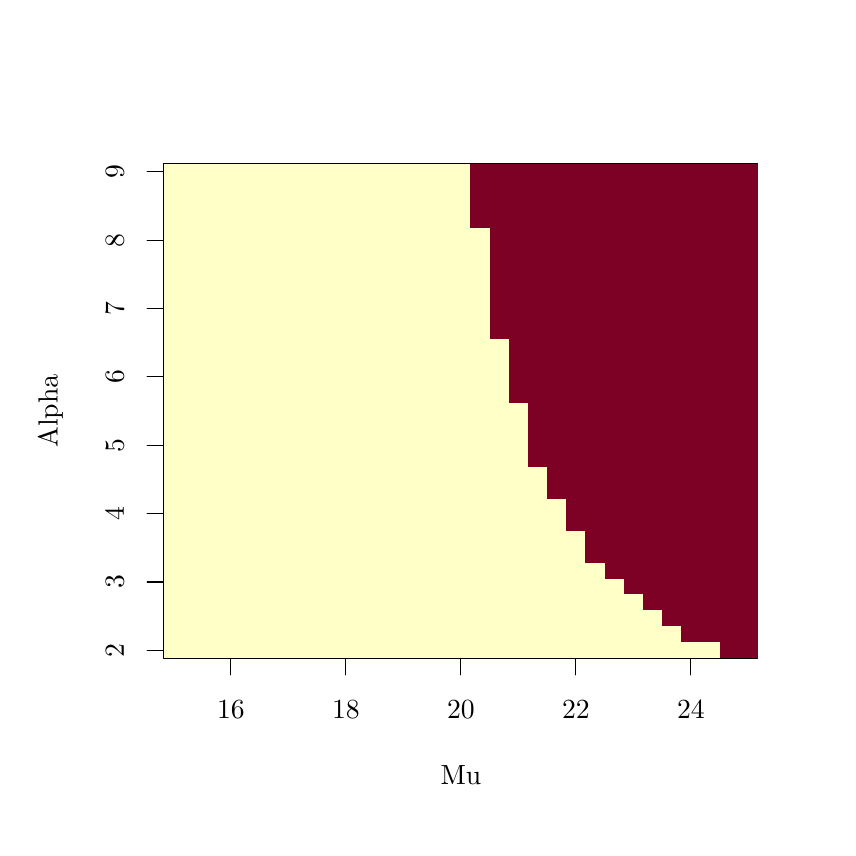
\begin{tikzpicture}[x=1pt,y=1pt]
\definecolor{fillColor}{RGB}{255,255,255}
\path[use as bounding box,fill=fillColor,fill opacity=0.00] (0,0) rectangle (289.08,289.08);
\begin{scope}
\path[clip] (  0.00,  0.00) rectangle (289.08,289.08);
\definecolor{drawColor}{RGB}{0,0,0}

\path[draw=drawColor,line width= 0.4pt,line join=round,line cap=round] ( 73.44, 61.20) -- (239.64, 61.20);

\path[draw=drawColor,line width= 0.4pt,line join=round,line cap=round] ( 73.44, 61.20) -- ( 73.44, 55.20);

\path[draw=drawColor,line width= 0.4pt,line join=round,line cap=round] (114.99, 61.20) -- (114.99, 55.20);

\path[draw=drawColor,line width= 0.4pt,line join=round,line cap=round] (156.54, 61.20) -- (156.54, 55.20);

\path[draw=drawColor,line width= 0.4pt,line join=round,line cap=round] (198.09, 61.20) -- (198.09, 55.20);

\path[draw=drawColor,line width= 0.4pt,line join=round,line cap=round] (239.64, 61.20) -- (239.64, 55.20);

\node[text=drawColor,anchor=base,inner sep=0pt, outer sep=0pt, scale=  1.00] at ( 73.44, 39.60) {16};

\node[text=drawColor,anchor=base,inner sep=0pt, outer sep=0pt, scale=  1.00] at (114.99, 39.60) {18};

\node[text=drawColor,anchor=base,inner sep=0pt, outer sep=0pt, scale=  1.00] at (156.54, 39.60) {20};

\node[text=drawColor,anchor=base,inner sep=0pt, outer sep=0pt, scale=  1.00] at (198.09, 39.60) {22};

\node[text=drawColor,anchor=base,inner sep=0pt, outer sep=0pt, scale=  1.00] at (239.64, 39.60) {24};

\path[draw=drawColor,line width= 0.4pt,line join=round,line cap=round] ( 49.20, 64.08) -- ( 49.20,237.00);

\path[draw=drawColor,line width= 0.4pt,line join=round,line cap=round] ( 49.20, 64.08) -- ( 43.20, 64.08);

\path[draw=drawColor,line width= 0.4pt,line join=round,line cap=round] ( 49.20, 88.78) -- ( 43.20, 88.78);

\path[draw=drawColor,line width= 0.4pt,line join=round,line cap=round] ( 49.20,113.49) -- ( 43.20,113.49);

\path[draw=drawColor,line width= 0.4pt,line join=round,line cap=round] ( 49.20,138.19) -- ( 43.20,138.19);

\path[draw=drawColor,line width= 0.4pt,line join=round,line cap=round] ( 49.20,162.89) -- ( 43.20,162.89);

\path[draw=drawColor,line width= 0.4pt,line join=round,line cap=round] ( 49.20,187.59) -- ( 43.20,187.59);

\path[draw=drawColor,line width= 0.4pt,line join=round,line cap=round] ( 49.20,212.30) -- ( 43.20,212.30);

\path[draw=drawColor,line width= 0.4pt,line join=round,line cap=round] ( 49.20,237.00) -- ( 43.20,237.00);

\node[text=drawColor,rotate= 90.00,anchor=base,inner sep=0pt, outer sep=0pt, scale=  1.00] at ( 34.80, 64.08) {2};

\node[text=drawColor,rotate= 90.00,anchor=base,inner sep=0pt, outer sep=0pt, scale=  1.00] at ( 34.80, 88.78) {3};

\node[text=drawColor,rotate= 90.00,anchor=base,inner sep=0pt, outer sep=0pt, scale=  1.00] at ( 34.80,113.49) {4};

\node[text=drawColor,rotate= 90.00,anchor=base,inner sep=0pt, outer sep=0pt, scale=  1.00] at ( 34.80,138.19) {5};

\node[text=drawColor,rotate= 90.00,anchor=base,inner sep=0pt, outer sep=0pt, scale=  1.00] at ( 34.80,162.89) {6};

\node[text=drawColor,rotate= 90.00,anchor=base,inner sep=0pt, outer sep=0pt, scale=  1.00] at ( 34.80,187.59) {7};

\node[text=drawColor,rotate= 90.00,anchor=base,inner sep=0pt, outer sep=0pt, scale=  1.00] at ( 34.80,212.30) {8};

\node[text=drawColor,rotate= 90.00,anchor=base,inner sep=0pt, outer sep=0pt, scale=  1.00] at ( 34.80,237.00) {9};

\path[draw=drawColor,line width= 0.4pt,line join=round,line cap=round] ( 49.20, 61.20) --
	(263.88, 61.20) --
	(263.88,239.88) --
	( 49.20,239.88) --
	( 49.20, 61.20);
\end{scope}
\begin{scope}
\path[clip] (  0.00,  0.00) rectangle (289.08,289.08);
\definecolor{drawColor}{RGB}{0,0,0}

\node[text=drawColor,anchor=base,inner sep=0pt, outer sep=0pt, scale=  1.00] at (156.54, 15.60) {Mu};

\node[text=drawColor,rotate= 90.00,anchor=base,inner sep=0pt, outer sep=0pt, scale=  1.00] at ( 10.80,150.54) {Alpha};
\end{scope}
\begin{scope}
\path[clip] ( 49.20, 61.20) rectangle (263.88,239.88);
\definecolor{fillColor}{RGB}{255,255,200}

\path[fill=fillColor] ( 49.20, 61.20) rectangle ( 56.13, 66.96);

\path[fill=fillColor] ( 49.20, 66.96) rectangle ( 56.13, 72.73);

\path[fill=fillColor] ( 49.20, 72.73) rectangle ( 56.13, 78.49);

\path[fill=fillColor] ( 49.20, 78.49) rectangle ( 56.13, 84.26);

\path[fill=fillColor] ( 49.20, 84.26) rectangle ( 56.13, 90.02);

\path[fill=fillColor] ( 49.20, 90.02) rectangle ( 56.13, 95.78);

\path[fill=fillColor] ( 49.20, 95.78) rectangle ( 56.13,101.55);

\path[fill=fillColor] ( 49.20,101.55) rectangle ( 56.13,107.31);

\path[fill=fillColor] ( 49.20,107.31) rectangle ( 56.13,113.07);

\path[fill=fillColor] ( 49.20,113.07) rectangle ( 56.13,118.84);

\path[fill=fillColor] ( 49.20,118.84) rectangle ( 56.13,124.60);

\path[fill=fillColor] ( 49.20,124.60) rectangle ( 56.13,130.37);

\path[fill=fillColor] ( 49.20,130.37) rectangle ( 56.13,136.13);

\path[fill=fillColor] ( 49.20,136.13) rectangle ( 56.13,141.89);

\path[fill=fillColor] ( 49.20,141.89) rectangle ( 56.13,147.66);

\path[fill=fillColor] ( 49.20,147.66) rectangle ( 56.13,153.42);

\path[fill=fillColor] ( 49.20,153.42) rectangle ( 56.13,159.19);

\path[fill=fillColor] ( 49.20,159.19) rectangle ( 56.13,164.95);

\path[fill=fillColor] ( 49.20,164.95) rectangle ( 56.13,170.71);

\path[fill=fillColor] ( 49.20,170.71) rectangle ( 56.13,176.48);

\path[fill=fillColor] ( 49.20,176.48) rectangle ( 56.13,182.24);

\path[fill=fillColor] ( 49.20,182.24) rectangle ( 56.13,188.01);

\path[fill=fillColor] ( 49.20,188.01) rectangle ( 56.13,193.77);

\path[fill=fillColor] ( 49.20,193.77) rectangle ( 56.13,199.53);

\path[fill=fillColor] ( 49.20,199.53) rectangle ( 56.13,205.30);

\path[fill=fillColor] ( 49.20,205.30) rectangle ( 56.13,211.06);

\path[fill=fillColor] ( 49.20,211.06) rectangle ( 56.13,216.82);

\path[fill=fillColor] ( 49.20,216.82) rectangle ( 56.13,222.59);

\path[fill=fillColor] ( 49.20,222.59) rectangle ( 56.13,228.35);

\path[fill=fillColor] ( 49.20,228.35) rectangle ( 56.13,234.12);

\path[fill=fillColor] ( 49.20,234.12) rectangle ( 56.13,239.88);

\path[fill=fillColor] ( 56.13, 61.20) rectangle ( 63.05, 66.96);

\path[fill=fillColor] ( 56.13, 66.96) rectangle ( 63.05, 72.73);

\path[fill=fillColor] ( 56.13, 72.73) rectangle ( 63.05, 78.49);

\path[fill=fillColor] ( 56.13, 78.49) rectangle ( 63.05, 84.26);

\path[fill=fillColor] ( 56.13, 84.26) rectangle ( 63.05, 90.02);

\path[fill=fillColor] ( 56.13, 90.02) rectangle ( 63.05, 95.78);

\path[fill=fillColor] ( 56.13, 95.78) rectangle ( 63.05,101.55);

\path[fill=fillColor] ( 56.13,101.55) rectangle ( 63.05,107.31);

\path[fill=fillColor] ( 56.13,107.31) rectangle ( 63.05,113.07);

\path[fill=fillColor] ( 56.13,113.07) rectangle ( 63.05,118.84);

\path[fill=fillColor] ( 56.13,118.84) rectangle ( 63.05,124.60);

\path[fill=fillColor] ( 56.13,124.60) rectangle ( 63.05,130.37);

\path[fill=fillColor] ( 56.13,130.37) rectangle ( 63.05,136.13);

\path[fill=fillColor] ( 56.13,136.13) rectangle ( 63.05,141.89);

\path[fill=fillColor] ( 56.13,141.89) rectangle ( 63.05,147.66);

\path[fill=fillColor] ( 56.13,147.66) rectangle ( 63.05,153.42);

\path[fill=fillColor] ( 56.13,153.42) rectangle ( 63.05,159.19);

\path[fill=fillColor] ( 56.13,159.19) rectangle ( 63.05,164.95);

\path[fill=fillColor] ( 56.13,164.95) rectangle ( 63.05,170.71);

\path[fill=fillColor] ( 56.13,170.71) rectangle ( 63.05,176.48);

\path[fill=fillColor] ( 56.13,176.48) rectangle ( 63.05,182.24);

\path[fill=fillColor] ( 56.13,182.24) rectangle ( 63.05,188.01);

\path[fill=fillColor] ( 56.13,188.01) rectangle ( 63.05,193.77);

\path[fill=fillColor] ( 56.13,193.77) rectangle ( 63.05,199.53);

\path[fill=fillColor] ( 56.13,199.53) rectangle ( 63.05,205.30);

\path[fill=fillColor] ( 56.13,205.30) rectangle ( 63.05,211.06);

\path[fill=fillColor] ( 56.13,211.06) rectangle ( 63.05,216.82);

\path[fill=fillColor] ( 56.13,216.82) rectangle ( 63.05,222.59);

\path[fill=fillColor] ( 56.13,222.59) rectangle ( 63.05,228.35);

\path[fill=fillColor] ( 56.13,228.35) rectangle ( 63.05,234.12);

\path[fill=fillColor] ( 56.13,234.12) rectangle ( 63.05,239.88);

\path[fill=fillColor] ( 63.05, 61.20) rectangle ( 69.98, 66.96);

\path[fill=fillColor] ( 63.05, 66.96) rectangle ( 69.98, 72.73);

\path[fill=fillColor] ( 63.05, 72.73) rectangle ( 69.98, 78.49);

\path[fill=fillColor] ( 63.05, 78.49) rectangle ( 69.98, 84.26);

\path[fill=fillColor] ( 63.05, 84.26) rectangle ( 69.98, 90.02);

\path[fill=fillColor] ( 63.05, 90.02) rectangle ( 69.98, 95.78);

\path[fill=fillColor] ( 63.05, 95.78) rectangle ( 69.98,101.55);

\path[fill=fillColor] ( 63.05,101.55) rectangle ( 69.98,107.31);

\path[fill=fillColor] ( 63.05,107.31) rectangle ( 69.98,113.07);

\path[fill=fillColor] ( 63.05,113.07) rectangle ( 69.98,118.84);

\path[fill=fillColor] ( 63.05,118.84) rectangle ( 69.98,124.60);

\path[fill=fillColor] ( 63.05,124.60) rectangle ( 69.98,130.37);

\path[fill=fillColor] ( 63.05,130.37) rectangle ( 69.98,136.13);

\path[fill=fillColor] ( 63.05,136.13) rectangle ( 69.98,141.89);

\path[fill=fillColor] ( 63.05,141.89) rectangle ( 69.98,147.66);

\path[fill=fillColor] ( 63.05,147.66) rectangle ( 69.98,153.42);

\path[fill=fillColor] ( 63.05,153.42) rectangle ( 69.98,159.19);

\path[fill=fillColor] ( 63.05,159.19) rectangle ( 69.98,164.95);

\path[fill=fillColor] ( 63.05,164.95) rectangle ( 69.98,170.71);

\path[fill=fillColor] ( 63.05,170.71) rectangle ( 69.98,176.48);

\path[fill=fillColor] ( 63.05,176.48) rectangle ( 69.98,182.24);

\path[fill=fillColor] ( 63.05,182.24) rectangle ( 69.98,188.01);

\path[fill=fillColor] ( 63.05,188.01) rectangle ( 69.98,193.77);

\path[fill=fillColor] ( 63.05,193.77) rectangle ( 69.98,199.53);

\path[fill=fillColor] ( 63.05,199.53) rectangle ( 69.98,205.30);

\path[fill=fillColor] ( 63.05,205.30) rectangle ( 69.98,211.06);

\path[fill=fillColor] ( 63.05,211.06) rectangle ( 69.98,216.82);

\path[fill=fillColor] ( 63.05,216.82) rectangle ( 69.98,222.59);

\path[fill=fillColor] ( 63.05,222.59) rectangle ( 69.98,228.35);

\path[fill=fillColor] ( 63.05,228.35) rectangle ( 69.98,234.12);

\path[fill=fillColor] ( 63.05,234.12) rectangle ( 69.98,239.88);

\path[fill=fillColor] ( 69.98, 61.20) rectangle ( 76.90, 66.96);

\path[fill=fillColor] ( 69.98, 66.96) rectangle ( 76.90, 72.73);

\path[fill=fillColor] ( 69.98, 72.73) rectangle ( 76.90, 78.49);

\path[fill=fillColor] ( 69.98, 78.49) rectangle ( 76.90, 84.26);

\path[fill=fillColor] ( 69.98, 84.26) rectangle ( 76.90, 90.02);

\path[fill=fillColor] ( 69.98, 90.02) rectangle ( 76.90, 95.78);

\path[fill=fillColor] ( 69.98, 95.78) rectangle ( 76.90,101.55);

\path[fill=fillColor] ( 69.98,101.55) rectangle ( 76.90,107.31);

\path[fill=fillColor] ( 69.98,107.31) rectangle ( 76.90,113.07);

\path[fill=fillColor] ( 69.98,113.07) rectangle ( 76.90,118.84);

\path[fill=fillColor] ( 69.98,118.84) rectangle ( 76.90,124.60);

\path[fill=fillColor] ( 69.98,124.60) rectangle ( 76.90,130.37);

\path[fill=fillColor] ( 69.98,130.37) rectangle ( 76.90,136.13);

\path[fill=fillColor] ( 69.98,136.13) rectangle ( 76.90,141.89);

\path[fill=fillColor] ( 69.98,141.89) rectangle ( 76.90,147.66);

\path[fill=fillColor] ( 69.98,147.66) rectangle ( 76.90,153.42);

\path[fill=fillColor] ( 69.98,153.42) rectangle ( 76.90,159.19);

\path[fill=fillColor] ( 69.98,159.19) rectangle ( 76.90,164.95);

\path[fill=fillColor] ( 69.98,164.95) rectangle ( 76.90,170.71);

\path[fill=fillColor] ( 69.98,170.71) rectangle ( 76.90,176.48);

\path[fill=fillColor] ( 69.98,176.48) rectangle ( 76.90,182.24);

\path[fill=fillColor] ( 69.98,182.24) rectangle ( 76.90,188.01);

\path[fill=fillColor] ( 69.98,188.01) rectangle ( 76.90,193.77);

\path[fill=fillColor] ( 69.98,193.77) rectangle ( 76.90,199.53);

\path[fill=fillColor] ( 69.98,199.53) rectangle ( 76.90,205.30);

\path[fill=fillColor] ( 69.98,205.30) rectangle ( 76.90,211.06);

\path[fill=fillColor] ( 69.98,211.06) rectangle ( 76.90,216.82);

\path[fill=fillColor] ( 69.98,216.82) rectangle ( 76.90,222.59);

\path[fill=fillColor] ( 69.98,222.59) rectangle ( 76.90,228.35);

\path[fill=fillColor] ( 69.98,228.35) rectangle ( 76.90,234.12);

\path[fill=fillColor] ( 69.98,234.12) rectangle ( 76.90,239.88);

\path[fill=fillColor] ( 76.90, 61.20) rectangle ( 83.83, 66.96);

\path[fill=fillColor] ( 76.90, 66.96) rectangle ( 83.83, 72.73);

\path[fill=fillColor] ( 76.90, 72.73) rectangle ( 83.83, 78.49);

\path[fill=fillColor] ( 76.90, 78.49) rectangle ( 83.83, 84.26);

\path[fill=fillColor] ( 76.90, 84.26) rectangle ( 83.83, 90.02);

\path[fill=fillColor] ( 76.90, 90.02) rectangle ( 83.83, 95.78);

\path[fill=fillColor] ( 76.90, 95.78) rectangle ( 83.83,101.55);

\path[fill=fillColor] ( 76.90,101.55) rectangle ( 83.83,107.31);

\path[fill=fillColor] ( 76.90,107.31) rectangle ( 83.83,113.07);

\path[fill=fillColor] ( 76.90,113.07) rectangle ( 83.83,118.84);

\path[fill=fillColor] ( 76.90,118.84) rectangle ( 83.83,124.60);

\path[fill=fillColor] ( 76.90,124.60) rectangle ( 83.83,130.37);

\path[fill=fillColor] ( 76.90,130.37) rectangle ( 83.83,136.13);

\path[fill=fillColor] ( 76.90,136.13) rectangle ( 83.83,141.89);

\path[fill=fillColor] ( 76.90,141.89) rectangle ( 83.83,147.66);

\path[fill=fillColor] ( 76.90,147.66) rectangle ( 83.83,153.42);

\path[fill=fillColor] ( 76.90,153.42) rectangle ( 83.83,159.19);

\path[fill=fillColor] ( 76.90,159.19) rectangle ( 83.83,164.95);

\path[fill=fillColor] ( 76.90,164.95) rectangle ( 83.83,170.71);

\path[fill=fillColor] ( 76.90,170.71) rectangle ( 83.83,176.48);

\path[fill=fillColor] ( 76.90,176.48) rectangle ( 83.83,182.24);

\path[fill=fillColor] ( 76.90,182.24) rectangle ( 83.83,188.01);

\path[fill=fillColor] ( 76.90,188.01) rectangle ( 83.83,193.77);

\path[fill=fillColor] ( 76.90,193.77) rectangle ( 83.83,199.53);

\path[fill=fillColor] ( 76.90,199.53) rectangle ( 83.83,205.30);

\path[fill=fillColor] ( 76.90,205.30) rectangle ( 83.83,211.06);

\path[fill=fillColor] ( 76.90,211.06) rectangle ( 83.83,216.82);

\path[fill=fillColor] ( 76.90,216.82) rectangle ( 83.83,222.59);

\path[fill=fillColor] ( 76.90,222.59) rectangle ( 83.83,228.35);

\path[fill=fillColor] ( 76.90,228.35) rectangle ( 83.83,234.12);

\path[fill=fillColor] ( 76.90,234.12) rectangle ( 83.83,239.88);

\path[fill=fillColor] ( 83.83, 61.20) rectangle ( 90.75, 66.96);

\path[fill=fillColor] ( 83.83, 66.96) rectangle ( 90.75, 72.73);

\path[fill=fillColor] ( 83.83, 72.73) rectangle ( 90.75, 78.49);

\path[fill=fillColor] ( 83.83, 78.49) rectangle ( 90.75, 84.26);

\path[fill=fillColor] ( 83.83, 84.26) rectangle ( 90.75, 90.02);

\path[fill=fillColor] ( 83.83, 90.02) rectangle ( 90.75, 95.78);

\path[fill=fillColor] ( 83.83, 95.78) rectangle ( 90.75,101.55);

\path[fill=fillColor] ( 83.83,101.55) rectangle ( 90.75,107.31);

\path[fill=fillColor] ( 83.83,107.31) rectangle ( 90.75,113.07);

\path[fill=fillColor] ( 83.83,113.07) rectangle ( 90.75,118.84);

\path[fill=fillColor] ( 83.83,118.84) rectangle ( 90.75,124.60);

\path[fill=fillColor] ( 83.83,124.60) rectangle ( 90.75,130.37);

\path[fill=fillColor] ( 83.83,130.37) rectangle ( 90.75,136.13);

\path[fill=fillColor] ( 83.83,136.13) rectangle ( 90.75,141.89);

\path[fill=fillColor] ( 83.83,141.89) rectangle ( 90.75,147.66);

\path[fill=fillColor] ( 83.83,147.66) rectangle ( 90.75,153.42);

\path[fill=fillColor] ( 83.83,153.42) rectangle ( 90.75,159.19);

\path[fill=fillColor] ( 83.83,159.19) rectangle ( 90.75,164.95);

\path[fill=fillColor] ( 83.83,164.95) rectangle ( 90.75,170.71);

\path[fill=fillColor] ( 83.83,170.71) rectangle ( 90.75,176.48);

\path[fill=fillColor] ( 83.83,176.48) rectangle ( 90.75,182.24);

\path[fill=fillColor] ( 83.83,182.24) rectangle ( 90.75,188.01);

\path[fill=fillColor] ( 83.83,188.01) rectangle ( 90.75,193.77);

\path[fill=fillColor] ( 83.83,193.77) rectangle ( 90.75,199.53);

\path[fill=fillColor] ( 83.83,199.53) rectangle ( 90.75,205.30);

\path[fill=fillColor] ( 83.83,205.30) rectangle ( 90.75,211.06);

\path[fill=fillColor] ( 83.83,211.06) rectangle ( 90.75,216.82);

\path[fill=fillColor] ( 83.83,216.82) rectangle ( 90.75,222.59);

\path[fill=fillColor] ( 83.83,222.59) rectangle ( 90.75,228.35);

\path[fill=fillColor] ( 83.83,228.35) rectangle ( 90.75,234.12);

\path[fill=fillColor] ( 83.83,234.12) rectangle ( 90.75,239.88);

\path[fill=fillColor] ( 90.75, 61.20) rectangle ( 97.68, 66.96);

\path[fill=fillColor] ( 90.75, 66.96) rectangle ( 97.68, 72.73);

\path[fill=fillColor] ( 90.75, 72.73) rectangle ( 97.68, 78.49);

\path[fill=fillColor] ( 90.75, 78.49) rectangle ( 97.68, 84.26);

\path[fill=fillColor] ( 90.75, 84.26) rectangle ( 97.68, 90.02);

\path[fill=fillColor] ( 90.75, 90.02) rectangle ( 97.68, 95.78);

\path[fill=fillColor] ( 90.75, 95.78) rectangle ( 97.68,101.55);

\path[fill=fillColor] ( 90.75,101.55) rectangle ( 97.68,107.31);

\path[fill=fillColor] ( 90.75,107.31) rectangle ( 97.68,113.07);

\path[fill=fillColor] ( 90.75,113.07) rectangle ( 97.68,118.84);

\path[fill=fillColor] ( 90.75,118.84) rectangle ( 97.68,124.60);

\path[fill=fillColor] ( 90.75,124.60) rectangle ( 97.68,130.37);

\path[fill=fillColor] ( 90.75,130.37) rectangle ( 97.68,136.13);

\path[fill=fillColor] ( 90.75,136.13) rectangle ( 97.68,141.89);

\path[fill=fillColor] ( 90.75,141.89) rectangle ( 97.68,147.66);

\path[fill=fillColor] ( 90.75,147.66) rectangle ( 97.68,153.42);

\path[fill=fillColor] ( 90.75,153.42) rectangle ( 97.68,159.19);

\path[fill=fillColor] ( 90.75,159.19) rectangle ( 97.68,164.95);

\path[fill=fillColor] ( 90.75,164.95) rectangle ( 97.68,170.71);

\path[fill=fillColor] ( 90.75,170.71) rectangle ( 97.68,176.48);

\path[fill=fillColor] ( 90.75,176.48) rectangle ( 97.68,182.24);

\path[fill=fillColor] ( 90.75,182.24) rectangle ( 97.68,188.01);

\path[fill=fillColor] ( 90.75,188.01) rectangle ( 97.68,193.77);

\path[fill=fillColor] ( 90.75,193.77) rectangle ( 97.68,199.53);

\path[fill=fillColor] ( 90.75,199.53) rectangle ( 97.68,205.30);

\path[fill=fillColor] ( 90.75,205.30) rectangle ( 97.68,211.06);

\path[fill=fillColor] ( 90.75,211.06) rectangle ( 97.68,216.82);

\path[fill=fillColor] ( 90.75,216.82) rectangle ( 97.68,222.59);

\path[fill=fillColor] ( 90.75,222.59) rectangle ( 97.68,228.35);

\path[fill=fillColor] ( 90.75,228.35) rectangle ( 97.68,234.12);

\path[fill=fillColor] ( 90.75,234.12) rectangle ( 97.68,239.88);

\path[fill=fillColor] ( 97.68, 61.20) rectangle (104.60, 66.96);

\path[fill=fillColor] ( 97.68, 66.96) rectangle (104.60, 72.73);

\path[fill=fillColor] ( 97.68, 72.73) rectangle (104.60, 78.49);

\path[fill=fillColor] ( 97.68, 78.49) rectangle (104.60, 84.26);

\path[fill=fillColor] ( 97.68, 84.26) rectangle (104.60, 90.02);

\path[fill=fillColor] ( 97.68, 90.02) rectangle (104.60, 95.78);

\path[fill=fillColor] ( 97.68, 95.78) rectangle (104.60,101.55);

\path[fill=fillColor] ( 97.68,101.55) rectangle (104.60,107.31);

\path[fill=fillColor] ( 97.68,107.31) rectangle (104.60,113.07);

\path[fill=fillColor] ( 97.68,113.07) rectangle (104.60,118.84);

\path[fill=fillColor] ( 97.68,118.84) rectangle (104.60,124.60);

\path[fill=fillColor] ( 97.68,124.60) rectangle (104.60,130.37);

\path[fill=fillColor] ( 97.68,130.37) rectangle (104.60,136.13);

\path[fill=fillColor] ( 97.68,136.13) rectangle (104.60,141.89);

\path[fill=fillColor] ( 97.68,141.89) rectangle (104.60,147.66);

\path[fill=fillColor] ( 97.68,147.66) rectangle (104.60,153.42);

\path[fill=fillColor] ( 97.68,153.42) rectangle (104.60,159.19);

\path[fill=fillColor] ( 97.68,159.19) rectangle (104.60,164.95);

\path[fill=fillColor] ( 97.68,164.95) rectangle (104.60,170.71);

\path[fill=fillColor] ( 97.68,170.71) rectangle (104.60,176.48);

\path[fill=fillColor] ( 97.68,176.48) rectangle (104.60,182.24);

\path[fill=fillColor] ( 97.68,182.24) rectangle (104.60,188.01);

\path[fill=fillColor] ( 97.68,188.01) rectangle (104.60,193.77);

\path[fill=fillColor] ( 97.68,193.77) rectangle (104.60,199.53);

\path[fill=fillColor] ( 97.68,199.53) rectangle (104.60,205.30);

\path[fill=fillColor] ( 97.68,205.30) rectangle (104.60,211.06);

\path[fill=fillColor] ( 97.68,211.06) rectangle (104.60,216.82);

\path[fill=fillColor] ( 97.68,216.82) rectangle (104.60,222.59);

\path[fill=fillColor] ( 97.68,222.59) rectangle (104.60,228.35);

\path[fill=fillColor] ( 97.68,228.35) rectangle (104.60,234.12);

\path[fill=fillColor] ( 97.68,234.12) rectangle (104.60,239.88);

\path[fill=fillColor] (104.60, 61.20) rectangle (111.53, 66.96);

\path[fill=fillColor] (104.60, 66.96) rectangle (111.53, 72.73);

\path[fill=fillColor] (104.60, 72.73) rectangle (111.53, 78.49);

\path[fill=fillColor] (104.60, 78.49) rectangle (111.53, 84.26);

\path[fill=fillColor] (104.60, 84.26) rectangle (111.53, 90.02);

\path[fill=fillColor] (104.60, 90.02) rectangle (111.53, 95.78);

\path[fill=fillColor] (104.60, 95.78) rectangle (111.53,101.55);

\path[fill=fillColor] (104.60,101.55) rectangle (111.53,107.31);

\path[fill=fillColor] (104.60,107.31) rectangle (111.53,113.07);

\path[fill=fillColor] (104.60,113.07) rectangle (111.53,118.84);

\path[fill=fillColor] (104.60,118.84) rectangle (111.53,124.60);

\path[fill=fillColor] (104.60,124.60) rectangle (111.53,130.37);

\path[fill=fillColor] (104.60,130.37) rectangle (111.53,136.13);

\path[fill=fillColor] (104.60,136.13) rectangle (111.53,141.89);

\path[fill=fillColor] (104.60,141.89) rectangle (111.53,147.66);

\path[fill=fillColor] (104.60,147.66) rectangle (111.53,153.42);

\path[fill=fillColor] (104.60,153.42) rectangle (111.53,159.19);

\path[fill=fillColor] (104.60,159.19) rectangle (111.53,164.95);

\path[fill=fillColor] (104.60,164.95) rectangle (111.53,170.71);

\path[fill=fillColor] (104.60,170.71) rectangle (111.53,176.48);

\path[fill=fillColor] (104.60,176.48) rectangle (111.53,182.24);

\path[fill=fillColor] (104.60,182.24) rectangle (111.53,188.01);

\path[fill=fillColor] (104.60,188.01) rectangle (111.53,193.77);

\path[fill=fillColor] (104.60,193.77) rectangle (111.53,199.53);

\path[fill=fillColor] (104.60,199.53) rectangle (111.53,205.30);

\path[fill=fillColor] (104.60,205.30) rectangle (111.53,211.06);

\path[fill=fillColor] (104.60,211.06) rectangle (111.53,216.82);

\path[fill=fillColor] (104.60,216.82) rectangle (111.53,222.59);

\path[fill=fillColor] (104.60,222.59) rectangle (111.53,228.35);

\path[fill=fillColor] (104.60,228.35) rectangle (111.53,234.12);

\path[fill=fillColor] (104.60,234.12) rectangle (111.53,239.88);

\path[fill=fillColor] (111.53, 61.20) rectangle (118.45, 66.96);

\path[fill=fillColor] (111.53, 66.96) rectangle (118.45, 72.73);

\path[fill=fillColor] (111.53, 72.73) rectangle (118.45, 78.49);

\path[fill=fillColor] (111.53, 78.49) rectangle (118.45, 84.26);

\path[fill=fillColor] (111.53, 84.26) rectangle (118.45, 90.02);

\path[fill=fillColor] (111.53, 90.02) rectangle (118.45, 95.78);

\path[fill=fillColor] (111.53, 95.78) rectangle (118.45,101.55);

\path[fill=fillColor] (111.53,101.55) rectangle (118.45,107.31);

\path[fill=fillColor] (111.53,107.31) rectangle (118.45,113.07);

\path[fill=fillColor] (111.53,113.07) rectangle (118.45,118.84);

\path[fill=fillColor] (111.53,118.84) rectangle (118.45,124.60);

\path[fill=fillColor] (111.53,124.60) rectangle (118.45,130.37);

\path[fill=fillColor] (111.53,130.37) rectangle (118.45,136.13);

\path[fill=fillColor] (111.53,136.13) rectangle (118.45,141.89);

\path[fill=fillColor] (111.53,141.89) rectangle (118.45,147.66);

\path[fill=fillColor] (111.53,147.66) rectangle (118.45,153.42);

\path[fill=fillColor] (111.53,153.42) rectangle (118.45,159.19);

\path[fill=fillColor] (111.53,159.19) rectangle (118.45,164.95);

\path[fill=fillColor] (111.53,164.95) rectangle (118.45,170.71);

\path[fill=fillColor] (111.53,170.71) rectangle (118.45,176.48);

\path[fill=fillColor] (111.53,176.48) rectangle (118.45,182.24);

\path[fill=fillColor] (111.53,182.24) rectangle (118.45,188.01);

\path[fill=fillColor] (111.53,188.01) rectangle (118.45,193.77);

\path[fill=fillColor] (111.53,193.77) rectangle (118.45,199.53);

\path[fill=fillColor] (111.53,199.53) rectangle (118.45,205.30);

\path[fill=fillColor] (111.53,205.30) rectangle (118.45,211.06);

\path[fill=fillColor] (111.53,211.06) rectangle (118.45,216.82);

\path[fill=fillColor] (111.53,216.82) rectangle (118.45,222.59);

\path[fill=fillColor] (111.53,222.59) rectangle (118.45,228.35);

\path[fill=fillColor] (111.53,228.35) rectangle (118.45,234.12);

\path[fill=fillColor] (111.53,234.12) rectangle (118.45,239.88);

\path[fill=fillColor] (118.45, 61.20) rectangle (125.38, 66.96);

\path[fill=fillColor] (118.45, 66.96) rectangle (125.38, 72.73);

\path[fill=fillColor] (118.45, 72.73) rectangle (125.38, 78.49);

\path[fill=fillColor] (118.45, 78.49) rectangle (125.38, 84.26);

\path[fill=fillColor] (118.45, 84.26) rectangle (125.38, 90.02);

\path[fill=fillColor] (118.45, 90.02) rectangle (125.38, 95.78);

\path[fill=fillColor] (118.45, 95.78) rectangle (125.38,101.55);

\path[fill=fillColor] (118.45,101.55) rectangle (125.38,107.31);

\path[fill=fillColor] (118.45,107.31) rectangle (125.38,113.07);

\path[fill=fillColor] (118.45,113.07) rectangle (125.38,118.84);

\path[fill=fillColor] (118.45,118.84) rectangle (125.38,124.60);

\path[fill=fillColor] (118.45,124.60) rectangle (125.38,130.37);

\path[fill=fillColor] (118.45,130.37) rectangle (125.38,136.13);

\path[fill=fillColor] (118.45,136.13) rectangle (125.38,141.89);

\path[fill=fillColor] (118.45,141.89) rectangle (125.38,147.66);

\path[fill=fillColor] (118.45,147.66) rectangle (125.38,153.42);

\path[fill=fillColor] (118.45,153.42) rectangle (125.38,159.19);

\path[fill=fillColor] (118.45,159.19) rectangle (125.38,164.95);

\path[fill=fillColor] (118.45,164.95) rectangle (125.38,170.71);

\path[fill=fillColor] (118.45,170.71) rectangle (125.38,176.48);

\path[fill=fillColor] (118.45,176.48) rectangle (125.38,182.24);

\path[fill=fillColor] (118.45,182.24) rectangle (125.38,188.01);

\path[fill=fillColor] (118.45,188.01) rectangle (125.38,193.77);

\path[fill=fillColor] (118.45,193.77) rectangle (125.38,199.53);

\path[fill=fillColor] (118.45,199.53) rectangle (125.38,205.30);

\path[fill=fillColor] (118.45,205.30) rectangle (125.38,211.06);

\path[fill=fillColor] (118.45,211.06) rectangle (125.38,216.82);

\path[fill=fillColor] (118.45,216.82) rectangle (125.38,222.59);

\path[fill=fillColor] (118.45,222.59) rectangle (125.38,228.35);

\path[fill=fillColor] (118.45,228.35) rectangle (125.38,234.12);

\path[fill=fillColor] (118.45,234.12) rectangle (125.38,239.88);

\path[fill=fillColor] (125.38, 61.20) rectangle (132.30, 66.96);

\path[fill=fillColor] (125.38, 66.96) rectangle (132.30, 72.73);

\path[fill=fillColor] (125.38, 72.73) rectangle (132.30, 78.49);

\path[fill=fillColor] (125.38, 78.49) rectangle (132.30, 84.26);

\path[fill=fillColor] (125.38, 84.26) rectangle (132.30, 90.02);

\path[fill=fillColor] (125.38, 90.02) rectangle (132.30, 95.78);

\path[fill=fillColor] (125.38, 95.78) rectangle (132.30,101.55);

\path[fill=fillColor] (125.38,101.55) rectangle (132.30,107.31);

\path[fill=fillColor] (125.38,107.31) rectangle (132.30,113.07);

\path[fill=fillColor] (125.38,113.07) rectangle (132.30,118.84);

\path[fill=fillColor] (125.38,118.84) rectangle (132.30,124.60);

\path[fill=fillColor] (125.38,124.60) rectangle (132.30,130.37);

\path[fill=fillColor] (125.38,130.37) rectangle (132.30,136.13);

\path[fill=fillColor] (125.38,136.13) rectangle (132.30,141.89);

\path[fill=fillColor] (125.38,141.89) rectangle (132.30,147.66);

\path[fill=fillColor] (125.38,147.66) rectangle (132.30,153.42);

\path[fill=fillColor] (125.38,153.42) rectangle (132.30,159.19);

\path[fill=fillColor] (125.38,159.19) rectangle (132.30,164.95);

\path[fill=fillColor] (125.38,164.95) rectangle (132.30,170.71);

\path[fill=fillColor] (125.38,170.71) rectangle (132.30,176.48);

\path[fill=fillColor] (125.38,176.48) rectangle (132.30,182.24);

\path[fill=fillColor] (125.38,182.24) rectangle (132.30,188.01);

\path[fill=fillColor] (125.38,188.01) rectangle (132.30,193.77);

\path[fill=fillColor] (125.38,193.77) rectangle (132.30,199.53);

\path[fill=fillColor] (125.38,199.53) rectangle (132.30,205.30);

\path[fill=fillColor] (125.38,205.30) rectangle (132.30,211.06);

\path[fill=fillColor] (125.38,211.06) rectangle (132.30,216.82);

\path[fill=fillColor] (125.38,216.82) rectangle (132.30,222.59);

\path[fill=fillColor] (125.38,222.59) rectangle (132.30,228.35);

\path[fill=fillColor] (125.38,228.35) rectangle (132.30,234.12);

\path[fill=fillColor] (125.38,234.12) rectangle (132.30,239.88);

\path[fill=fillColor] (132.30, 61.20) rectangle (139.23, 66.96);

\path[fill=fillColor] (132.30, 66.96) rectangle (139.23, 72.73);

\path[fill=fillColor] (132.30, 72.73) rectangle (139.23, 78.49);

\path[fill=fillColor] (132.30, 78.49) rectangle (139.23, 84.26);

\path[fill=fillColor] (132.30, 84.26) rectangle (139.23, 90.02);

\path[fill=fillColor] (132.30, 90.02) rectangle (139.23, 95.78);

\path[fill=fillColor] (132.30, 95.78) rectangle (139.23,101.55);

\path[fill=fillColor] (132.30,101.55) rectangle (139.23,107.31);

\path[fill=fillColor] (132.30,107.31) rectangle (139.23,113.07);

\path[fill=fillColor] (132.30,113.07) rectangle (139.23,118.84);

\path[fill=fillColor] (132.30,118.84) rectangle (139.23,124.60);

\path[fill=fillColor] (132.30,124.60) rectangle (139.23,130.37);

\path[fill=fillColor] (132.30,130.37) rectangle (139.23,136.13);

\path[fill=fillColor] (132.30,136.13) rectangle (139.23,141.89);

\path[fill=fillColor] (132.30,141.89) rectangle (139.23,147.66);

\path[fill=fillColor] (132.30,147.66) rectangle (139.23,153.42);

\path[fill=fillColor] (132.30,153.42) rectangle (139.23,159.19);

\path[fill=fillColor] (132.30,159.19) rectangle (139.23,164.95);

\path[fill=fillColor] (132.30,164.95) rectangle (139.23,170.71);

\path[fill=fillColor] (132.30,170.71) rectangle (139.23,176.48);

\path[fill=fillColor] (132.30,176.48) rectangle (139.23,182.24);

\path[fill=fillColor] (132.30,182.24) rectangle (139.23,188.01);

\path[fill=fillColor] (132.30,188.01) rectangle (139.23,193.77);

\path[fill=fillColor] (132.30,193.77) rectangle (139.23,199.53);

\path[fill=fillColor] (132.30,199.53) rectangle (139.23,205.30);

\path[fill=fillColor] (132.30,205.30) rectangle (139.23,211.06);

\path[fill=fillColor] (132.30,211.06) rectangle (139.23,216.82);

\path[fill=fillColor] (132.30,216.82) rectangle (139.23,222.59);

\path[fill=fillColor] (132.30,222.59) rectangle (139.23,228.35);

\path[fill=fillColor] (132.30,228.35) rectangle (139.23,234.12);

\path[fill=fillColor] (132.30,234.12) rectangle (139.23,239.88);

\path[fill=fillColor] (139.23, 61.20) rectangle (146.15, 66.96);

\path[fill=fillColor] (139.23, 66.96) rectangle (146.15, 72.73);

\path[fill=fillColor] (139.23, 72.73) rectangle (146.15, 78.49);

\path[fill=fillColor] (139.23, 78.49) rectangle (146.15, 84.26);

\path[fill=fillColor] (139.23, 84.26) rectangle (146.15, 90.02);

\path[fill=fillColor] (139.23, 90.02) rectangle (146.15, 95.78);

\path[fill=fillColor] (139.23, 95.78) rectangle (146.15,101.55);

\path[fill=fillColor] (139.23,101.55) rectangle (146.15,107.31);

\path[fill=fillColor] (139.23,107.31) rectangle (146.15,113.07);

\path[fill=fillColor] (139.23,113.07) rectangle (146.15,118.84);

\path[fill=fillColor] (139.23,118.84) rectangle (146.15,124.60);

\path[fill=fillColor] (139.23,124.60) rectangle (146.15,130.37);

\path[fill=fillColor] (139.23,130.37) rectangle (146.15,136.13);

\path[fill=fillColor] (139.23,136.13) rectangle (146.15,141.89);

\path[fill=fillColor] (139.23,141.89) rectangle (146.15,147.66);

\path[fill=fillColor] (139.23,147.66) rectangle (146.15,153.42);

\path[fill=fillColor] (139.23,153.42) rectangle (146.15,159.19);

\path[fill=fillColor] (139.23,159.19) rectangle (146.15,164.95);

\path[fill=fillColor] (139.23,164.95) rectangle (146.15,170.71);

\path[fill=fillColor] (139.23,170.71) rectangle (146.15,176.48);

\path[fill=fillColor] (139.23,176.48) rectangle (146.15,182.24);

\path[fill=fillColor] (139.23,182.24) rectangle (146.15,188.01);

\path[fill=fillColor] (139.23,188.01) rectangle (146.15,193.77);

\path[fill=fillColor] (139.23,193.77) rectangle (146.15,199.53);

\path[fill=fillColor] (139.23,199.53) rectangle (146.15,205.30);

\path[fill=fillColor] (139.23,205.30) rectangle (146.15,211.06);

\path[fill=fillColor] (139.23,211.06) rectangle (146.15,216.82);

\path[fill=fillColor] (139.23,216.82) rectangle (146.15,222.59);

\path[fill=fillColor] (139.23,222.59) rectangle (146.15,228.35);

\path[fill=fillColor] (139.23,228.35) rectangle (146.15,234.12);

\path[fill=fillColor] (139.23,234.12) rectangle (146.15,239.88);

\path[fill=fillColor] (146.15, 61.20) rectangle (153.08, 66.96);

\path[fill=fillColor] (146.15, 66.96) rectangle (153.08, 72.73);

\path[fill=fillColor] (146.15, 72.73) rectangle (153.08, 78.49);

\path[fill=fillColor] (146.15, 78.49) rectangle (153.08, 84.26);

\path[fill=fillColor] (146.15, 84.26) rectangle (153.08, 90.02);

\path[fill=fillColor] (146.15, 90.02) rectangle (153.08, 95.78);

\path[fill=fillColor] (146.15, 95.78) rectangle (153.08,101.55);

\path[fill=fillColor] (146.15,101.55) rectangle (153.08,107.31);

\path[fill=fillColor] (146.15,107.31) rectangle (153.08,113.07);

\path[fill=fillColor] (146.15,113.07) rectangle (153.08,118.84);

\path[fill=fillColor] (146.15,118.84) rectangle (153.08,124.60);

\path[fill=fillColor] (146.15,124.60) rectangle (153.08,130.37);

\path[fill=fillColor] (146.15,130.37) rectangle (153.08,136.13);

\path[fill=fillColor] (146.15,136.13) rectangle (153.08,141.89);

\path[fill=fillColor] (146.15,141.89) rectangle (153.08,147.66);

\path[fill=fillColor] (146.15,147.66) rectangle (153.08,153.42);

\path[fill=fillColor] (146.15,153.42) rectangle (153.08,159.19);

\path[fill=fillColor] (146.15,159.19) rectangle (153.08,164.95);

\path[fill=fillColor] (146.15,164.95) rectangle (153.08,170.71);

\path[fill=fillColor] (146.15,170.71) rectangle (153.08,176.48);

\path[fill=fillColor] (146.15,176.48) rectangle (153.08,182.24);

\path[fill=fillColor] (146.15,182.24) rectangle (153.08,188.01);

\path[fill=fillColor] (146.15,188.01) rectangle (153.08,193.77);

\path[fill=fillColor] (146.15,193.77) rectangle (153.08,199.53);

\path[fill=fillColor] (146.15,199.53) rectangle (153.08,205.30);

\path[fill=fillColor] (146.15,205.30) rectangle (153.08,211.06);

\path[fill=fillColor] (146.15,211.06) rectangle (153.08,216.82);

\path[fill=fillColor] (146.15,216.82) rectangle (153.08,222.59);

\path[fill=fillColor] (146.15,222.59) rectangle (153.08,228.35);

\path[fill=fillColor] (146.15,228.35) rectangle (153.08,234.12);

\path[fill=fillColor] (146.15,234.12) rectangle (153.08,239.88);

\path[fill=fillColor] (153.08, 61.20) rectangle (160.00, 66.96);

\path[fill=fillColor] (153.08, 66.96) rectangle (160.00, 72.73);

\path[fill=fillColor] (153.08, 72.73) rectangle (160.00, 78.49);

\path[fill=fillColor] (153.08, 78.49) rectangle (160.00, 84.26);

\path[fill=fillColor] (153.08, 84.26) rectangle (160.00, 90.02);

\path[fill=fillColor] (153.08, 90.02) rectangle (160.00, 95.78);

\path[fill=fillColor] (153.08, 95.78) rectangle (160.00,101.55);

\path[fill=fillColor] (153.08,101.55) rectangle (160.00,107.31);

\path[fill=fillColor] (153.08,107.31) rectangle (160.00,113.07);

\path[fill=fillColor] (153.08,113.07) rectangle (160.00,118.84);

\path[fill=fillColor] (153.08,118.84) rectangle (160.00,124.60);

\path[fill=fillColor] (153.08,124.60) rectangle (160.00,130.37);

\path[fill=fillColor] (153.08,130.37) rectangle (160.00,136.13);

\path[fill=fillColor] (153.08,136.13) rectangle (160.00,141.89);

\path[fill=fillColor] (153.08,141.89) rectangle (160.00,147.66);

\path[fill=fillColor] (153.08,147.66) rectangle (160.00,153.42);

\path[fill=fillColor] (153.08,153.42) rectangle (160.00,159.19);

\path[fill=fillColor] (153.08,159.19) rectangle (160.00,164.95);

\path[fill=fillColor] (153.08,164.95) rectangle (160.00,170.71);

\path[fill=fillColor] (153.08,170.71) rectangle (160.00,176.48);

\path[fill=fillColor] (153.08,176.48) rectangle (160.00,182.24);

\path[fill=fillColor] (153.08,182.24) rectangle (160.00,188.01);

\path[fill=fillColor] (153.08,188.01) rectangle (160.00,193.77);

\path[fill=fillColor] (153.08,193.77) rectangle (160.00,199.53);

\path[fill=fillColor] (153.08,199.53) rectangle (160.00,205.30);

\path[fill=fillColor] (153.08,205.30) rectangle (160.00,211.06);

\path[fill=fillColor] (153.08,211.06) rectangle (160.00,216.82);

\path[fill=fillColor] (153.08,216.82) rectangle (160.00,222.59);

\path[fill=fillColor] (153.08,222.59) rectangle (160.00,228.35);

\path[fill=fillColor] (153.08,228.35) rectangle (160.00,234.12);

\path[fill=fillColor] (153.08,234.12) rectangle (160.00,239.88);

\path[fill=fillColor] (160.00, 61.20) rectangle (166.93, 66.96);

\path[fill=fillColor] (160.00, 66.96) rectangle (166.93, 72.73);

\path[fill=fillColor] (160.00, 72.73) rectangle (166.93, 78.49);

\path[fill=fillColor] (160.00, 78.49) rectangle (166.93, 84.26);

\path[fill=fillColor] (160.00, 84.26) rectangle (166.93, 90.02);

\path[fill=fillColor] (160.00, 90.02) rectangle (166.93, 95.78);

\path[fill=fillColor] (160.00, 95.78) rectangle (166.93,101.55);

\path[fill=fillColor] (160.00,101.55) rectangle (166.93,107.31);

\path[fill=fillColor] (160.00,107.31) rectangle (166.93,113.07);

\path[fill=fillColor] (160.00,113.07) rectangle (166.93,118.84);

\path[fill=fillColor] (160.00,118.84) rectangle (166.93,124.60);

\path[fill=fillColor] (160.00,124.60) rectangle (166.93,130.37);

\path[fill=fillColor] (160.00,130.37) rectangle (166.93,136.13);

\path[fill=fillColor] (160.00,136.13) rectangle (166.93,141.89);

\path[fill=fillColor] (160.00,141.89) rectangle (166.93,147.66);

\path[fill=fillColor] (160.00,147.66) rectangle (166.93,153.42);

\path[fill=fillColor] (160.00,153.42) rectangle (166.93,159.19);

\path[fill=fillColor] (160.00,159.19) rectangle (166.93,164.95);

\path[fill=fillColor] (160.00,164.95) rectangle (166.93,170.71);

\path[fill=fillColor] (160.00,170.71) rectangle (166.93,176.48);

\path[fill=fillColor] (160.00,176.48) rectangle (166.93,182.24);

\path[fill=fillColor] (160.00,182.24) rectangle (166.93,188.01);

\path[fill=fillColor] (160.00,188.01) rectangle (166.93,193.77);

\path[fill=fillColor] (160.00,193.77) rectangle (166.93,199.53);

\path[fill=fillColor] (160.00,199.53) rectangle (166.93,205.30);

\path[fill=fillColor] (160.00,205.30) rectangle (166.93,211.06);

\path[fill=fillColor] (160.00,211.06) rectangle (166.93,216.82);
\definecolor{fillColor}{RGB}{125,0,37}

\path[fill=fillColor] (160.00,216.82) rectangle (166.93,222.59);

\path[fill=fillColor] (160.00,222.59) rectangle (166.93,228.35);

\path[fill=fillColor] (160.00,228.35) rectangle (166.93,234.12);

\path[fill=fillColor] (160.00,234.12) rectangle (166.93,239.88);
\definecolor{fillColor}{RGB}{255,255,200}

\path[fill=fillColor] (166.93, 61.20) rectangle (173.85, 66.96);

\path[fill=fillColor] (166.93, 66.96) rectangle (173.85, 72.73);

\path[fill=fillColor] (166.93, 72.73) rectangle (173.85, 78.49);

\path[fill=fillColor] (166.93, 78.49) rectangle (173.85, 84.26);

\path[fill=fillColor] (166.93, 84.26) rectangle (173.85, 90.02);

\path[fill=fillColor] (166.93, 90.02) rectangle (173.85, 95.78);

\path[fill=fillColor] (166.93, 95.78) rectangle (173.85,101.55);

\path[fill=fillColor] (166.93,101.55) rectangle (173.85,107.31);

\path[fill=fillColor] (166.93,107.31) rectangle (173.85,113.07);

\path[fill=fillColor] (166.93,113.07) rectangle (173.85,118.84);

\path[fill=fillColor] (166.93,118.84) rectangle (173.85,124.60);

\path[fill=fillColor] (166.93,124.60) rectangle (173.85,130.37);

\path[fill=fillColor] (166.93,130.37) rectangle (173.85,136.13);

\path[fill=fillColor] (166.93,136.13) rectangle (173.85,141.89);

\path[fill=fillColor] (166.93,141.89) rectangle (173.85,147.66);

\path[fill=fillColor] (166.93,147.66) rectangle (173.85,153.42);

\path[fill=fillColor] (166.93,153.42) rectangle (173.85,159.19);

\path[fill=fillColor] (166.93,159.19) rectangle (173.85,164.95);

\path[fill=fillColor] (166.93,164.95) rectangle (173.85,170.71);

\path[fill=fillColor] (166.93,170.71) rectangle (173.85,176.48);
\definecolor{fillColor}{RGB}{125,0,37}

\path[fill=fillColor] (166.93,176.48) rectangle (173.85,182.24);

\path[fill=fillColor] (166.93,182.24) rectangle (173.85,188.01);

\path[fill=fillColor] (166.93,188.01) rectangle (173.85,193.77);

\path[fill=fillColor] (166.93,193.77) rectangle (173.85,199.53);

\path[fill=fillColor] (166.93,199.53) rectangle (173.85,205.30);

\path[fill=fillColor] (166.93,205.30) rectangle (173.85,211.06);

\path[fill=fillColor] (166.93,211.06) rectangle (173.85,216.82);

\path[fill=fillColor] (166.93,216.82) rectangle (173.85,222.59);

\path[fill=fillColor] (166.93,222.59) rectangle (173.85,228.35);

\path[fill=fillColor] (166.93,228.35) rectangle (173.85,234.12);

\path[fill=fillColor] (166.93,234.12) rectangle (173.85,239.88);
\definecolor{fillColor}{RGB}{255,255,200}

\path[fill=fillColor] (173.85, 61.20) rectangle (180.78, 66.96);

\path[fill=fillColor] (173.85, 66.96) rectangle (180.78, 72.73);

\path[fill=fillColor] (173.85, 72.73) rectangle (180.78, 78.49);

\path[fill=fillColor] (173.85, 78.49) rectangle (180.78, 84.26);

\path[fill=fillColor] (173.85, 84.26) rectangle (180.78, 90.02);

\path[fill=fillColor] (173.85, 90.02) rectangle (180.78, 95.78);

\path[fill=fillColor] (173.85, 95.78) rectangle (180.78,101.55);

\path[fill=fillColor] (173.85,101.55) rectangle (180.78,107.31);

\path[fill=fillColor] (173.85,107.31) rectangle (180.78,113.07);

\path[fill=fillColor] (173.85,113.07) rectangle (180.78,118.84);

\path[fill=fillColor] (173.85,118.84) rectangle (180.78,124.60);

\path[fill=fillColor] (173.85,124.60) rectangle (180.78,130.37);

\path[fill=fillColor] (173.85,130.37) rectangle (180.78,136.13);

\path[fill=fillColor] (173.85,136.13) rectangle (180.78,141.89);

\path[fill=fillColor] (173.85,141.89) rectangle (180.78,147.66);

\path[fill=fillColor] (173.85,147.66) rectangle (180.78,153.42);
\definecolor{fillColor}{RGB}{125,0,37}

\path[fill=fillColor] (173.85,153.42) rectangle (180.78,159.19);

\path[fill=fillColor] (173.85,159.19) rectangle (180.78,164.95);

\path[fill=fillColor] (173.85,164.95) rectangle (180.78,170.71);

\path[fill=fillColor] (173.85,170.71) rectangle (180.78,176.48);

\path[fill=fillColor] (173.85,176.48) rectangle (180.78,182.24);

\path[fill=fillColor] (173.85,182.24) rectangle (180.78,188.01);

\path[fill=fillColor] (173.85,188.01) rectangle (180.78,193.77);

\path[fill=fillColor] (173.85,193.77) rectangle (180.78,199.53);

\path[fill=fillColor] (173.85,199.53) rectangle (180.78,205.30);

\path[fill=fillColor] (173.85,205.30) rectangle (180.78,211.06);

\path[fill=fillColor] (173.85,211.06) rectangle (180.78,216.82);

\path[fill=fillColor] (173.85,216.82) rectangle (180.78,222.59);

\path[fill=fillColor] (173.85,222.59) rectangle (180.78,228.35);

\path[fill=fillColor] (173.85,228.35) rectangle (180.78,234.12);

\path[fill=fillColor] (173.85,234.12) rectangle (180.78,239.88);
\definecolor{fillColor}{RGB}{255,255,200}

\path[fill=fillColor] (180.78, 61.20) rectangle (187.70, 66.96);

\path[fill=fillColor] (180.78, 66.96) rectangle (187.70, 72.73);

\path[fill=fillColor] (180.78, 72.73) rectangle (187.70, 78.49);

\path[fill=fillColor] (180.78, 78.49) rectangle (187.70, 84.26);

\path[fill=fillColor] (180.78, 84.26) rectangle (187.70, 90.02);

\path[fill=fillColor] (180.78, 90.02) rectangle (187.70, 95.78);

\path[fill=fillColor] (180.78, 95.78) rectangle (187.70,101.55);

\path[fill=fillColor] (180.78,101.55) rectangle (187.70,107.31);

\path[fill=fillColor] (180.78,107.31) rectangle (187.70,113.07);

\path[fill=fillColor] (180.78,113.07) rectangle (187.70,118.84);

\path[fill=fillColor] (180.78,118.84) rectangle (187.70,124.60);

\path[fill=fillColor] (180.78,124.60) rectangle (187.70,130.37);
\definecolor{fillColor}{RGB}{125,0,37}

\path[fill=fillColor] (180.78,130.37) rectangle (187.70,136.13);

\path[fill=fillColor] (180.78,136.13) rectangle (187.70,141.89);

\path[fill=fillColor] (180.78,141.89) rectangle (187.70,147.66);

\path[fill=fillColor] (180.78,147.66) rectangle (187.70,153.42);

\path[fill=fillColor] (180.78,153.42) rectangle (187.70,159.19);

\path[fill=fillColor] (180.78,159.19) rectangle (187.70,164.95);

\path[fill=fillColor] (180.78,164.95) rectangle (187.70,170.71);

\path[fill=fillColor] (180.78,170.71) rectangle (187.70,176.48);

\path[fill=fillColor] (180.78,176.48) rectangle (187.70,182.24);

\path[fill=fillColor] (180.78,182.24) rectangle (187.70,188.01);

\path[fill=fillColor] (180.78,188.01) rectangle (187.70,193.77);

\path[fill=fillColor] (180.78,193.77) rectangle (187.70,199.53);

\path[fill=fillColor] (180.78,199.53) rectangle (187.70,205.30);

\path[fill=fillColor] (180.78,205.30) rectangle (187.70,211.06);

\path[fill=fillColor] (180.78,211.06) rectangle (187.70,216.82);

\path[fill=fillColor] (180.78,216.82) rectangle (187.70,222.59);

\path[fill=fillColor] (180.78,222.59) rectangle (187.70,228.35);

\path[fill=fillColor] (180.78,228.35) rectangle (187.70,234.12);

\path[fill=fillColor] (180.78,234.12) rectangle (187.70,239.88);
\definecolor{fillColor}{RGB}{255,255,200}

\path[fill=fillColor] (187.70, 61.20) rectangle (194.63, 66.96);

\path[fill=fillColor] (187.70, 66.96) rectangle (194.63, 72.73);

\path[fill=fillColor] (187.70, 72.73) rectangle (194.63, 78.49);

\path[fill=fillColor] (187.70, 78.49) rectangle (194.63, 84.26);

\path[fill=fillColor] (187.70, 84.26) rectangle (194.63, 90.02);

\path[fill=fillColor] (187.70, 90.02) rectangle (194.63, 95.78);

\path[fill=fillColor] (187.70, 95.78) rectangle (194.63,101.55);

\path[fill=fillColor] (187.70,101.55) rectangle (194.63,107.31);

\path[fill=fillColor] (187.70,107.31) rectangle (194.63,113.07);

\path[fill=fillColor] (187.70,113.07) rectangle (194.63,118.84);
\definecolor{fillColor}{RGB}{125,0,37}

\path[fill=fillColor] (187.70,118.84) rectangle (194.63,124.60);

\path[fill=fillColor] (187.70,124.60) rectangle (194.63,130.37);

\path[fill=fillColor] (187.70,130.37) rectangle (194.63,136.13);

\path[fill=fillColor] (187.70,136.13) rectangle (194.63,141.89);

\path[fill=fillColor] (187.70,141.89) rectangle (194.63,147.66);

\path[fill=fillColor] (187.70,147.66) rectangle (194.63,153.42);

\path[fill=fillColor] (187.70,153.42) rectangle (194.63,159.19);

\path[fill=fillColor] (187.70,159.19) rectangle (194.63,164.95);

\path[fill=fillColor] (187.70,164.95) rectangle (194.63,170.71);

\path[fill=fillColor] (187.70,170.71) rectangle (194.63,176.48);

\path[fill=fillColor] (187.70,176.48) rectangle (194.63,182.24);

\path[fill=fillColor] (187.70,182.24) rectangle (194.63,188.01);

\path[fill=fillColor] (187.70,188.01) rectangle (194.63,193.77);

\path[fill=fillColor] (187.70,193.77) rectangle (194.63,199.53);

\path[fill=fillColor] (187.70,199.53) rectangle (194.63,205.30);

\path[fill=fillColor] (187.70,205.30) rectangle (194.63,211.06);

\path[fill=fillColor] (187.70,211.06) rectangle (194.63,216.82);

\path[fill=fillColor] (187.70,216.82) rectangle (194.63,222.59);

\path[fill=fillColor] (187.70,222.59) rectangle (194.63,228.35);

\path[fill=fillColor] (187.70,228.35) rectangle (194.63,234.12);

\path[fill=fillColor] (187.70,234.12) rectangle (194.63,239.88);
\definecolor{fillColor}{RGB}{255,255,200}

\path[fill=fillColor] (194.63, 61.20) rectangle (201.55, 66.96);

\path[fill=fillColor] (194.63, 66.96) rectangle (201.55, 72.73);

\path[fill=fillColor] (194.63, 72.73) rectangle (201.55, 78.49);

\path[fill=fillColor] (194.63, 78.49) rectangle (201.55, 84.26);

\path[fill=fillColor] (194.63, 84.26) rectangle (201.55, 90.02);

\path[fill=fillColor] (194.63, 90.02) rectangle (201.55, 95.78);

\path[fill=fillColor] (194.63, 95.78) rectangle (201.55,101.55);

\path[fill=fillColor] (194.63,101.55) rectangle (201.55,107.31);
\definecolor{fillColor}{RGB}{125,0,37}

\path[fill=fillColor] (194.63,107.31) rectangle (201.55,113.07);

\path[fill=fillColor] (194.63,113.07) rectangle (201.55,118.84);

\path[fill=fillColor] (194.63,118.84) rectangle (201.55,124.60);

\path[fill=fillColor] (194.63,124.60) rectangle (201.55,130.37);

\path[fill=fillColor] (194.63,130.37) rectangle (201.55,136.13);

\path[fill=fillColor] (194.63,136.13) rectangle (201.55,141.89);

\path[fill=fillColor] (194.63,141.89) rectangle (201.55,147.66);

\path[fill=fillColor] (194.63,147.66) rectangle (201.55,153.42);

\path[fill=fillColor] (194.63,153.42) rectangle (201.55,159.19);

\path[fill=fillColor] (194.63,159.19) rectangle (201.55,164.95);

\path[fill=fillColor] (194.63,164.95) rectangle (201.55,170.71);

\path[fill=fillColor] (194.63,170.71) rectangle (201.55,176.48);

\path[fill=fillColor] (194.63,176.48) rectangle (201.55,182.24);

\path[fill=fillColor] (194.63,182.24) rectangle (201.55,188.01);

\path[fill=fillColor] (194.63,188.01) rectangle (201.55,193.77);

\path[fill=fillColor] (194.63,193.77) rectangle (201.55,199.53);

\path[fill=fillColor] (194.63,199.53) rectangle (201.55,205.30);

\path[fill=fillColor] (194.63,205.30) rectangle (201.55,211.06);

\path[fill=fillColor] (194.63,211.06) rectangle (201.55,216.82);

\path[fill=fillColor] (194.63,216.82) rectangle (201.55,222.59);

\path[fill=fillColor] (194.63,222.59) rectangle (201.55,228.35);

\path[fill=fillColor] (194.63,228.35) rectangle (201.55,234.12);

\path[fill=fillColor] (194.63,234.12) rectangle (201.55,239.88);
\definecolor{fillColor}{RGB}{255,255,200}

\path[fill=fillColor] (201.55, 61.20) rectangle (208.48, 66.96);

\path[fill=fillColor] (201.55, 66.96) rectangle (208.48, 72.73);

\path[fill=fillColor] (201.55, 72.73) rectangle (208.48, 78.49);

\path[fill=fillColor] (201.55, 78.49) rectangle (208.48, 84.26);

\path[fill=fillColor] (201.55, 84.26) rectangle (208.48, 90.02);

\path[fill=fillColor] (201.55, 90.02) rectangle (208.48, 95.78);
\definecolor{fillColor}{RGB}{125,0,37}

\path[fill=fillColor] (201.55, 95.78) rectangle (208.48,101.55);

\path[fill=fillColor] (201.55,101.55) rectangle (208.48,107.31);

\path[fill=fillColor] (201.55,107.31) rectangle (208.48,113.07);

\path[fill=fillColor] (201.55,113.07) rectangle (208.48,118.84);

\path[fill=fillColor] (201.55,118.84) rectangle (208.48,124.60);

\path[fill=fillColor] (201.55,124.60) rectangle (208.48,130.37);

\path[fill=fillColor] (201.55,130.37) rectangle (208.48,136.13);

\path[fill=fillColor] (201.55,136.13) rectangle (208.48,141.89);

\path[fill=fillColor] (201.55,141.89) rectangle (208.48,147.66);

\path[fill=fillColor] (201.55,147.66) rectangle (208.48,153.42);

\path[fill=fillColor] (201.55,153.42) rectangle (208.48,159.19);

\path[fill=fillColor] (201.55,159.19) rectangle (208.48,164.95);

\path[fill=fillColor] (201.55,164.95) rectangle (208.48,170.71);

\path[fill=fillColor] (201.55,170.71) rectangle (208.48,176.48);

\path[fill=fillColor] (201.55,176.48) rectangle (208.48,182.24);

\path[fill=fillColor] (201.55,182.24) rectangle (208.48,188.01);

\path[fill=fillColor] (201.55,188.01) rectangle (208.48,193.77);

\path[fill=fillColor] (201.55,193.77) rectangle (208.48,199.53);

\path[fill=fillColor] (201.55,199.53) rectangle (208.48,205.30);

\path[fill=fillColor] (201.55,205.30) rectangle (208.48,211.06);

\path[fill=fillColor] (201.55,211.06) rectangle (208.48,216.82);

\path[fill=fillColor] (201.55,216.82) rectangle (208.48,222.59);

\path[fill=fillColor] (201.55,222.59) rectangle (208.48,228.35);

\path[fill=fillColor] (201.55,228.35) rectangle (208.48,234.12);

\path[fill=fillColor] (201.55,234.12) rectangle (208.48,239.88);
\definecolor{fillColor}{RGB}{255,255,200}

\path[fill=fillColor] (208.48, 61.20) rectangle (215.40, 66.96);

\path[fill=fillColor] (208.48, 66.96) rectangle (215.40, 72.73);

\path[fill=fillColor] (208.48, 72.73) rectangle (215.40, 78.49);

\path[fill=fillColor] (208.48, 78.49) rectangle (215.40, 84.26);

\path[fill=fillColor] (208.48, 84.26) rectangle (215.40, 90.02);
\definecolor{fillColor}{RGB}{125,0,37}

\path[fill=fillColor] (208.48, 90.02) rectangle (215.40, 95.78);

\path[fill=fillColor] (208.48, 95.78) rectangle (215.40,101.55);

\path[fill=fillColor] (208.48,101.55) rectangle (215.40,107.31);

\path[fill=fillColor] (208.48,107.31) rectangle (215.40,113.07);

\path[fill=fillColor] (208.48,113.07) rectangle (215.40,118.84);

\path[fill=fillColor] (208.48,118.84) rectangle (215.40,124.60);

\path[fill=fillColor] (208.48,124.60) rectangle (215.40,130.37);

\path[fill=fillColor] (208.48,130.37) rectangle (215.40,136.13);

\path[fill=fillColor] (208.48,136.13) rectangle (215.40,141.89);

\path[fill=fillColor] (208.48,141.89) rectangle (215.40,147.66);

\path[fill=fillColor] (208.48,147.66) rectangle (215.40,153.42);

\path[fill=fillColor] (208.48,153.42) rectangle (215.40,159.19);

\path[fill=fillColor] (208.48,159.19) rectangle (215.40,164.95);

\path[fill=fillColor] (208.48,164.95) rectangle (215.40,170.71);

\path[fill=fillColor] (208.48,170.71) rectangle (215.40,176.48);

\path[fill=fillColor] (208.48,176.48) rectangle (215.40,182.24);

\path[fill=fillColor] (208.48,182.24) rectangle (215.40,188.01);

\path[fill=fillColor] (208.48,188.01) rectangle (215.40,193.77);

\path[fill=fillColor] (208.48,193.77) rectangle (215.40,199.53);

\path[fill=fillColor] (208.48,199.53) rectangle (215.40,205.30);

\path[fill=fillColor] (208.48,205.30) rectangle (215.40,211.06);

\path[fill=fillColor] (208.48,211.06) rectangle (215.40,216.82);

\path[fill=fillColor] (208.48,216.82) rectangle (215.40,222.59);

\path[fill=fillColor] (208.48,222.59) rectangle (215.40,228.35);

\path[fill=fillColor] (208.48,228.35) rectangle (215.40,234.12);

\path[fill=fillColor] (208.48,234.12) rectangle (215.40,239.88);
\definecolor{fillColor}{RGB}{255,255,200}

\path[fill=fillColor] (215.40, 61.20) rectangle (222.33, 66.96);

\path[fill=fillColor] (215.40, 66.96) rectangle (222.33, 72.73);

\path[fill=fillColor] (215.40, 72.73) rectangle (222.33, 78.49);

\path[fill=fillColor] (215.40, 78.49) rectangle (222.33, 84.26);
\definecolor{fillColor}{RGB}{125,0,37}

\path[fill=fillColor] (215.40, 84.26) rectangle (222.33, 90.02);

\path[fill=fillColor] (215.40, 90.02) rectangle (222.33, 95.78);

\path[fill=fillColor] (215.40, 95.78) rectangle (222.33,101.55);

\path[fill=fillColor] (215.40,101.55) rectangle (222.33,107.31);

\path[fill=fillColor] (215.40,107.31) rectangle (222.33,113.07);

\path[fill=fillColor] (215.40,113.07) rectangle (222.33,118.84);

\path[fill=fillColor] (215.40,118.84) rectangle (222.33,124.60);

\path[fill=fillColor] (215.40,124.60) rectangle (222.33,130.37);

\path[fill=fillColor] (215.40,130.37) rectangle (222.33,136.13);

\path[fill=fillColor] (215.40,136.13) rectangle (222.33,141.89);

\path[fill=fillColor] (215.40,141.89) rectangle (222.33,147.66);

\path[fill=fillColor] (215.40,147.66) rectangle (222.33,153.42);

\path[fill=fillColor] (215.40,153.42) rectangle (222.33,159.19);

\path[fill=fillColor] (215.40,159.19) rectangle (222.33,164.95);

\path[fill=fillColor] (215.40,164.95) rectangle (222.33,170.71);

\path[fill=fillColor] (215.40,170.71) rectangle (222.33,176.48);

\path[fill=fillColor] (215.40,176.48) rectangle (222.33,182.24);

\path[fill=fillColor] (215.40,182.24) rectangle (222.33,188.01);

\path[fill=fillColor] (215.40,188.01) rectangle (222.33,193.77);

\path[fill=fillColor] (215.40,193.77) rectangle (222.33,199.53);

\path[fill=fillColor] (215.40,199.53) rectangle (222.33,205.30);

\path[fill=fillColor] (215.40,205.30) rectangle (222.33,211.06);

\path[fill=fillColor] (215.40,211.06) rectangle (222.33,216.82);

\path[fill=fillColor] (215.40,216.82) rectangle (222.33,222.59);

\path[fill=fillColor] (215.40,222.59) rectangle (222.33,228.35);

\path[fill=fillColor] (215.40,228.35) rectangle (222.33,234.12);

\path[fill=fillColor] (215.40,234.12) rectangle (222.33,239.88);
\definecolor{fillColor}{RGB}{255,255,200}

\path[fill=fillColor] (222.33, 61.20) rectangle (229.25, 66.96);

\path[fill=fillColor] (222.33, 66.96) rectangle (229.25, 72.73);

\path[fill=fillColor] (222.33, 72.73) rectangle (229.25, 78.49);
\definecolor{fillColor}{RGB}{125,0,37}

\path[fill=fillColor] (222.33, 78.49) rectangle (229.25, 84.26);

\path[fill=fillColor] (222.33, 84.26) rectangle (229.25, 90.02);

\path[fill=fillColor] (222.33, 90.02) rectangle (229.25, 95.78);

\path[fill=fillColor] (222.33, 95.78) rectangle (229.25,101.55);

\path[fill=fillColor] (222.33,101.55) rectangle (229.25,107.31);

\path[fill=fillColor] (222.33,107.31) rectangle (229.25,113.07);

\path[fill=fillColor] (222.33,113.07) rectangle (229.25,118.84);

\path[fill=fillColor] (222.33,118.84) rectangle (229.25,124.60);

\path[fill=fillColor] (222.33,124.60) rectangle (229.25,130.37);

\path[fill=fillColor] (222.33,130.37) rectangle (229.25,136.13);

\path[fill=fillColor] (222.33,136.13) rectangle (229.25,141.89);

\path[fill=fillColor] (222.33,141.89) rectangle (229.25,147.66);

\path[fill=fillColor] (222.33,147.66) rectangle (229.25,153.42);

\path[fill=fillColor] (222.33,153.42) rectangle (229.25,159.19);

\path[fill=fillColor] (222.33,159.19) rectangle (229.25,164.95);

\path[fill=fillColor] (222.33,164.95) rectangle (229.25,170.71);

\path[fill=fillColor] (222.33,170.71) rectangle (229.25,176.48);

\path[fill=fillColor] (222.33,176.48) rectangle (229.25,182.24);

\path[fill=fillColor] (222.33,182.24) rectangle (229.25,188.01);

\path[fill=fillColor] (222.33,188.01) rectangle (229.25,193.77);

\path[fill=fillColor] (222.33,193.77) rectangle (229.25,199.53);

\path[fill=fillColor] (222.33,199.53) rectangle (229.25,205.30);

\path[fill=fillColor] (222.33,205.30) rectangle (229.25,211.06);

\path[fill=fillColor] (222.33,211.06) rectangle (229.25,216.82);

\path[fill=fillColor] (222.33,216.82) rectangle (229.25,222.59);

\path[fill=fillColor] (222.33,222.59) rectangle (229.25,228.35);

\path[fill=fillColor] (222.33,228.35) rectangle (229.25,234.12);

\path[fill=fillColor] (222.33,234.12) rectangle (229.25,239.88);
\definecolor{fillColor}{RGB}{255,255,200}

\path[fill=fillColor] (229.25, 61.20) rectangle (236.18, 66.96);

\path[fill=fillColor] (229.25, 66.96) rectangle (236.18, 72.73);
\definecolor{fillColor}{RGB}{125,0,37}

\path[fill=fillColor] (229.25, 72.73) rectangle (236.18, 78.49);

\path[fill=fillColor] (229.25, 78.49) rectangle (236.18, 84.26);

\path[fill=fillColor] (229.25, 84.26) rectangle (236.18, 90.02);

\path[fill=fillColor] (229.25, 90.02) rectangle (236.18, 95.78);

\path[fill=fillColor] (229.25, 95.78) rectangle (236.18,101.55);

\path[fill=fillColor] (229.25,101.55) rectangle (236.18,107.31);

\path[fill=fillColor] (229.25,107.31) rectangle (236.18,113.07);

\path[fill=fillColor] (229.25,113.07) rectangle (236.18,118.84);

\path[fill=fillColor] (229.25,118.84) rectangle (236.18,124.60);

\path[fill=fillColor] (229.25,124.60) rectangle (236.18,130.37);

\path[fill=fillColor] (229.25,130.37) rectangle (236.18,136.13);

\path[fill=fillColor] (229.25,136.13) rectangle (236.18,141.89);

\path[fill=fillColor] (229.25,141.89) rectangle (236.18,147.66);

\path[fill=fillColor] (229.25,147.66) rectangle (236.18,153.42);

\path[fill=fillColor] (229.25,153.42) rectangle (236.18,159.19);

\path[fill=fillColor] (229.25,159.19) rectangle (236.18,164.95);

\path[fill=fillColor] (229.25,164.95) rectangle (236.18,170.71);

\path[fill=fillColor] (229.25,170.71) rectangle (236.18,176.48);

\path[fill=fillColor] (229.25,176.48) rectangle (236.18,182.24);

\path[fill=fillColor] (229.25,182.24) rectangle (236.18,188.01);

\path[fill=fillColor] (229.25,188.01) rectangle (236.18,193.77);

\path[fill=fillColor] (229.25,193.77) rectangle (236.18,199.53);

\path[fill=fillColor] (229.25,199.53) rectangle (236.18,205.30);

\path[fill=fillColor] (229.25,205.30) rectangle (236.18,211.06);

\path[fill=fillColor] (229.25,211.06) rectangle (236.18,216.82);

\path[fill=fillColor] (229.25,216.82) rectangle (236.18,222.59);

\path[fill=fillColor] (229.25,222.59) rectangle (236.18,228.35);

\path[fill=fillColor] (229.25,228.35) rectangle (236.18,234.12);

\path[fill=fillColor] (229.25,234.12) rectangle (236.18,239.88);
\definecolor{fillColor}{RGB}{255,255,200}

\path[fill=fillColor] (236.18, 61.20) rectangle (243.10, 66.96);
\definecolor{fillColor}{RGB}{125,0,37}

\path[fill=fillColor] (236.18, 66.96) rectangle (243.10, 72.73);

\path[fill=fillColor] (236.18, 72.73) rectangle (243.10, 78.49);

\path[fill=fillColor] (236.18, 78.49) rectangle (243.10, 84.26);

\path[fill=fillColor] (236.18, 84.26) rectangle (243.10, 90.02);

\path[fill=fillColor] (236.18, 90.02) rectangle (243.10, 95.78);

\path[fill=fillColor] (236.18, 95.78) rectangle (243.10,101.55);

\path[fill=fillColor] (236.18,101.55) rectangle (243.10,107.31);

\path[fill=fillColor] (236.18,107.31) rectangle (243.10,113.07);

\path[fill=fillColor] (236.18,113.07) rectangle (243.10,118.84);

\path[fill=fillColor] (236.18,118.84) rectangle (243.10,124.60);

\path[fill=fillColor] (236.18,124.60) rectangle (243.10,130.37);

\path[fill=fillColor] (236.18,130.37) rectangle (243.10,136.13);

\path[fill=fillColor] (236.18,136.13) rectangle (243.10,141.89);

\path[fill=fillColor] (236.18,141.89) rectangle (243.10,147.66);

\path[fill=fillColor] (236.18,147.66) rectangle (243.10,153.42);

\path[fill=fillColor] (236.18,153.42) rectangle (243.10,159.19);

\path[fill=fillColor] (236.18,159.19) rectangle (243.10,164.95);

\path[fill=fillColor] (236.18,164.95) rectangle (243.10,170.71);

\path[fill=fillColor] (236.18,170.71) rectangle (243.10,176.48);

\path[fill=fillColor] (236.18,176.48) rectangle (243.10,182.24);

\path[fill=fillColor] (236.18,182.24) rectangle (243.10,188.01);

\path[fill=fillColor] (236.18,188.01) rectangle (243.10,193.77);

\path[fill=fillColor] (236.18,193.77) rectangle (243.10,199.53);

\path[fill=fillColor] (236.18,199.53) rectangle (243.10,205.30);

\path[fill=fillColor] (236.18,205.30) rectangle (243.10,211.06);

\path[fill=fillColor] (236.18,211.06) rectangle (243.10,216.82);

\path[fill=fillColor] (236.18,216.82) rectangle (243.10,222.59);

\path[fill=fillColor] (236.18,222.59) rectangle (243.10,228.35);

\path[fill=fillColor] (236.18,228.35) rectangle (243.10,234.12);

\path[fill=fillColor] (236.18,234.12) rectangle (243.10,239.88);
\definecolor{fillColor}{RGB}{255,255,200}

\path[fill=fillColor] (243.10, 61.20) rectangle (250.03, 66.96);
\definecolor{fillColor}{RGB}{125,0,37}

\path[fill=fillColor] (243.10, 66.96) rectangle (250.03, 72.73);

\path[fill=fillColor] (243.10, 72.73) rectangle (250.03, 78.49);

\path[fill=fillColor] (243.10, 78.49) rectangle (250.03, 84.26);

\path[fill=fillColor] (243.10, 84.26) rectangle (250.03, 90.02);

\path[fill=fillColor] (243.10, 90.02) rectangle (250.03, 95.78);

\path[fill=fillColor] (243.10, 95.78) rectangle (250.03,101.55);

\path[fill=fillColor] (243.10,101.55) rectangle (250.03,107.31);

\path[fill=fillColor] (243.10,107.31) rectangle (250.03,113.07);

\path[fill=fillColor] (243.10,113.07) rectangle (250.03,118.84);

\path[fill=fillColor] (243.10,118.84) rectangle (250.03,124.60);

\path[fill=fillColor] (243.10,124.60) rectangle (250.03,130.37);

\path[fill=fillColor] (243.10,130.37) rectangle (250.03,136.13);

\path[fill=fillColor] (243.10,136.13) rectangle (250.03,141.89);

\path[fill=fillColor] (243.10,141.89) rectangle (250.03,147.66);

\path[fill=fillColor] (243.10,147.66) rectangle (250.03,153.42);

\path[fill=fillColor] (243.10,153.42) rectangle (250.03,159.19);

\path[fill=fillColor] (243.10,159.19) rectangle (250.03,164.95);

\path[fill=fillColor] (243.10,164.95) rectangle (250.03,170.71);

\path[fill=fillColor] (243.10,170.71) rectangle (250.03,176.48);

\path[fill=fillColor] (243.10,176.48) rectangle (250.03,182.24);

\path[fill=fillColor] (243.10,182.24) rectangle (250.03,188.01);

\path[fill=fillColor] (243.10,188.01) rectangle (250.03,193.77);

\path[fill=fillColor] (243.10,193.77) rectangle (250.03,199.53);

\path[fill=fillColor] (243.10,199.53) rectangle (250.03,205.30);

\path[fill=fillColor] (243.10,205.30) rectangle (250.03,211.06);

\path[fill=fillColor] (243.10,211.06) rectangle (250.03,216.82);

\path[fill=fillColor] (243.10,216.82) rectangle (250.03,222.59);

\path[fill=fillColor] (243.10,222.59) rectangle (250.03,228.35);

\path[fill=fillColor] (243.10,228.35) rectangle (250.03,234.12);

\path[fill=fillColor] (243.10,234.12) rectangle (250.03,239.88);

\path[fill=fillColor] (250.03, 61.20) rectangle (256.95, 66.96);

\path[fill=fillColor] (250.03, 66.96) rectangle (256.95, 72.73);

\path[fill=fillColor] (250.03, 72.73) rectangle (256.95, 78.49);

\path[fill=fillColor] (250.03, 78.49) rectangle (256.95, 84.26);

\path[fill=fillColor] (250.03, 84.26) rectangle (256.95, 90.02);

\path[fill=fillColor] (250.03, 90.02) rectangle (256.95, 95.78);

\path[fill=fillColor] (250.03, 95.78) rectangle (256.95,101.55);

\path[fill=fillColor] (250.03,101.55) rectangle (256.95,107.31);

\path[fill=fillColor] (250.03,107.31) rectangle (256.95,113.07);

\path[fill=fillColor] (250.03,113.07) rectangle (256.95,118.84);

\path[fill=fillColor] (250.03,118.84) rectangle (256.95,124.60);

\path[fill=fillColor] (250.03,124.60) rectangle (256.95,130.37);

\path[fill=fillColor] (250.03,130.37) rectangle (256.95,136.13);

\path[fill=fillColor] (250.03,136.13) rectangle (256.95,141.89);

\path[fill=fillColor] (250.03,141.89) rectangle (256.95,147.66);

\path[fill=fillColor] (250.03,147.66) rectangle (256.95,153.42);

\path[fill=fillColor] (250.03,153.42) rectangle (256.95,159.19);

\path[fill=fillColor] (250.03,159.19) rectangle (256.95,164.95);

\path[fill=fillColor] (250.03,164.95) rectangle (256.95,170.71);

\path[fill=fillColor] (250.03,170.71) rectangle (256.95,176.48);

\path[fill=fillColor] (250.03,176.48) rectangle (256.95,182.24);

\path[fill=fillColor] (250.03,182.24) rectangle (256.95,188.01);

\path[fill=fillColor] (250.03,188.01) rectangle (256.95,193.77);

\path[fill=fillColor] (250.03,193.77) rectangle (256.95,199.53);

\path[fill=fillColor] (250.03,199.53) rectangle (256.95,205.30);

\path[fill=fillColor] (250.03,205.30) rectangle (256.95,211.06);

\path[fill=fillColor] (250.03,211.06) rectangle (256.95,216.82);

\path[fill=fillColor] (250.03,216.82) rectangle (256.95,222.59);

\path[fill=fillColor] (250.03,222.59) rectangle (256.95,228.35);

\path[fill=fillColor] (250.03,228.35) rectangle (256.95,234.12);

\path[fill=fillColor] (250.03,234.12) rectangle (256.95,239.88);

\path[fill=fillColor] (256.95, 61.20) rectangle (263.88, 66.96);

\path[fill=fillColor] (256.95, 66.96) rectangle (263.88, 72.73);

\path[fill=fillColor] (256.95, 72.73) rectangle (263.88, 78.49);

\path[fill=fillColor] (256.95, 78.49) rectangle (263.88, 84.26);

\path[fill=fillColor] (256.95, 84.26) rectangle (263.88, 90.02);

\path[fill=fillColor] (256.95, 90.02) rectangle (263.88, 95.78);

\path[fill=fillColor] (256.95, 95.78) rectangle (263.88,101.55);

\path[fill=fillColor] (256.95,101.55) rectangle (263.88,107.31);

\path[fill=fillColor] (256.95,107.31) rectangle (263.88,113.07);

\path[fill=fillColor] (256.95,113.07) rectangle (263.88,118.84);

\path[fill=fillColor] (256.95,118.84) rectangle (263.88,124.60);

\path[fill=fillColor] (256.95,124.60) rectangle (263.88,130.37);

\path[fill=fillColor] (256.95,130.37) rectangle (263.88,136.13);

\path[fill=fillColor] (256.95,136.13) rectangle (263.88,141.89);

\path[fill=fillColor] (256.95,141.89) rectangle (263.88,147.66);

\path[fill=fillColor] (256.95,147.66) rectangle (263.88,153.42);

\path[fill=fillColor] (256.95,153.42) rectangle (263.88,159.19);

\path[fill=fillColor] (256.95,159.19) rectangle (263.88,164.95);

\path[fill=fillColor] (256.95,164.95) rectangle (263.88,170.71);

\path[fill=fillColor] (256.95,170.71) rectangle (263.88,176.48);

\path[fill=fillColor] (256.95,176.48) rectangle (263.88,182.24);

\path[fill=fillColor] (256.95,182.24) rectangle (263.88,188.01);

\path[fill=fillColor] (256.95,188.01) rectangle (263.88,193.77);

\path[fill=fillColor] (256.95,193.77) rectangle (263.88,199.53);

\path[fill=fillColor] (256.95,199.53) rectangle (263.88,205.30);

\path[fill=fillColor] (256.95,205.30) rectangle (263.88,211.06);

\path[fill=fillColor] (256.95,211.06) rectangle (263.88,216.82);

\path[fill=fillColor] (256.95,216.82) rectangle (263.88,222.59);

\path[fill=fillColor] (256.95,222.59) rectangle (263.88,228.35);

\path[fill=fillColor] (256.95,228.35) rectangle (263.88,234.12);

\path[fill=fillColor] (256.95,234.12) rectangle (263.88,239.88);
\end{scope}
\end{tikzpicture}

	\caption{The optimal decision for persons with mature knees visualized on
		the grid of $\mu$ and $\alpha$.
		Red signifies that the decision is to classify as adults, and white, as children.
	\label{fig:optimal_c}}
\end{figure}

\begin{figure}
	\centering
	% Created by tikzDevice version 0.12.3 on 2019-10-10 22:07:10
% !TEX encoding = UTF-8 Unicode
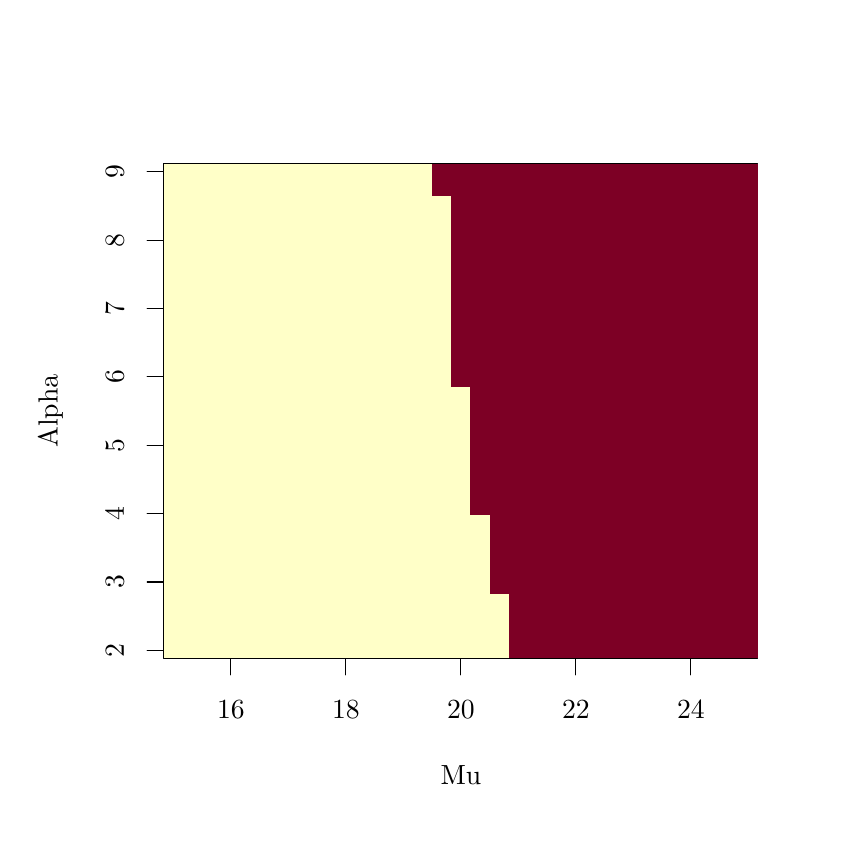
\begin{tikzpicture}[x=1pt,y=1pt]
\definecolor{fillColor}{RGB}{255,255,255}
\path[use as bounding box,fill=fillColor,fill opacity=0.00] (0,0) rectangle (289.08,289.08);
\begin{scope}
\path[clip] (  0.00,  0.00) rectangle (289.08,289.08);
\definecolor{drawColor}{RGB}{0,0,0}

\path[draw=drawColor,line width= 0.4pt,line join=round,line cap=round] ( 73.44, 61.20) -- (239.64, 61.20);

\path[draw=drawColor,line width= 0.4pt,line join=round,line cap=round] ( 73.44, 61.20) -- ( 73.44, 55.20);

\path[draw=drawColor,line width= 0.4pt,line join=round,line cap=round] (114.99, 61.20) -- (114.99, 55.20);

\path[draw=drawColor,line width= 0.4pt,line join=round,line cap=round] (156.54, 61.20) -- (156.54, 55.20);

\path[draw=drawColor,line width= 0.4pt,line join=round,line cap=round] (198.09, 61.20) -- (198.09, 55.20);

\path[draw=drawColor,line width= 0.4pt,line join=round,line cap=round] (239.64, 61.20) -- (239.64, 55.20);

\node[text=drawColor,anchor=base,inner sep=0pt, outer sep=0pt, scale=  1.00] at ( 73.44, 39.60) {16};

\node[text=drawColor,anchor=base,inner sep=0pt, outer sep=0pt, scale=  1.00] at (114.99, 39.60) {18};

\node[text=drawColor,anchor=base,inner sep=0pt, outer sep=0pt, scale=  1.00] at (156.54, 39.60) {20};

\node[text=drawColor,anchor=base,inner sep=0pt, outer sep=0pt, scale=  1.00] at (198.09, 39.60) {22};

\node[text=drawColor,anchor=base,inner sep=0pt, outer sep=0pt, scale=  1.00] at (239.64, 39.60) {24};

\path[draw=drawColor,line width= 0.4pt,line join=round,line cap=round] ( 49.20, 64.08) -- ( 49.20,237.00);

\path[draw=drawColor,line width= 0.4pt,line join=round,line cap=round] ( 49.20, 64.08) -- ( 43.20, 64.08);

\path[draw=drawColor,line width= 0.4pt,line join=round,line cap=round] ( 49.20, 88.78) -- ( 43.20, 88.78);

\path[draw=drawColor,line width= 0.4pt,line join=round,line cap=round] ( 49.20,113.49) -- ( 43.20,113.49);

\path[draw=drawColor,line width= 0.4pt,line join=round,line cap=round] ( 49.20,138.19) -- ( 43.20,138.19);

\path[draw=drawColor,line width= 0.4pt,line join=round,line cap=round] ( 49.20,162.89) -- ( 43.20,162.89);

\path[draw=drawColor,line width= 0.4pt,line join=round,line cap=round] ( 49.20,187.59) -- ( 43.20,187.59);

\path[draw=drawColor,line width= 0.4pt,line join=round,line cap=round] ( 49.20,212.30) -- ( 43.20,212.30);

\path[draw=drawColor,line width= 0.4pt,line join=round,line cap=round] ( 49.20,237.00) -- ( 43.20,237.00);

\node[text=drawColor,rotate= 90.00,anchor=base,inner sep=0pt, outer sep=0pt, scale=  1.00] at ( 34.80, 64.08) {2};

\node[text=drawColor,rotate= 90.00,anchor=base,inner sep=0pt, outer sep=0pt, scale=  1.00] at ( 34.80, 88.78) {3};

\node[text=drawColor,rotate= 90.00,anchor=base,inner sep=0pt, outer sep=0pt, scale=  1.00] at ( 34.80,113.49) {4};

\node[text=drawColor,rotate= 90.00,anchor=base,inner sep=0pt, outer sep=0pt, scale=  1.00] at ( 34.80,138.19) {5};

\node[text=drawColor,rotate= 90.00,anchor=base,inner sep=0pt, outer sep=0pt, scale=  1.00] at ( 34.80,162.89) {6};

\node[text=drawColor,rotate= 90.00,anchor=base,inner sep=0pt, outer sep=0pt, scale=  1.00] at ( 34.80,187.59) {7};

\node[text=drawColor,rotate= 90.00,anchor=base,inner sep=0pt, outer sep=0pt, scale=  1.00] at ( 34.80,212.30) {8};

\node[text=drawColor,rotate= 90.00,anchor=base,inner sep=0pt, outer sep=0pt, scale=  1.00] at ( 34.80,237.00) {9};

\path[draw=drawColor,line width= 0.4pt,line join=round,line cap=round] ( 49.20, 61.20) --
	(263.88, 61.20) --
	(263.88,239.88) --
	( 49.20,239.88) --
	( 49.20, 61.20);
\end{scope}
\begin{scope}
\path[clip] (  0.00,  0.00) rectangle (289.08,289.08);
\definecolor{drawColor}{RGB}{0,0,0}

\node[text=drawColor,anchor=base,inner sep=0pt, outer sep=0pt, scale=  1.00] at (156.54, 15.60) {Mu};

\node[text=drawColor,rotate= 90.00,anchor=base,inner sep=0pt, outer sep=0pt, scale=  1.00] at ( 10.80,150.54) {Alpha};
\end{scope}
\begin{scope}
\path[clip] ( 49.20, 61.20) rectangle (263.88,239.88);
\definecolor{fillColor}{RGB}{255,255,200}

\path[fill=fillColor] ( 49.20, 61.20) rectangle ( 56.13, 66.96);

\path[fill=fillColor] ( 49.20, 66.96) rectangle ( 56.13, 72.73);

\path[fill=fillColor] ( 49.20, 72.73) rectangle ( 56.13, 78.49);

\path[fill=fillColor] ( 49.20, 78.49) rectangle ( 56.13, 84.26);

\path[fill=fillColor] ( 49.20, 84.26) rectangle ( 56.13, 90.02);

\path[fill=fillColor] ( 49.20, 90.02) rectangle ( 56.13, 95.78);

\path[fill=fillColor] ( 49.20, 95.78) rectangle ( 56.13,101.55);

\path[fill=fillColor] ( 49.20,101.55) rectangle ( 56.13,107.31);

\path[fill=fillColor] ( 49.20,107.31) rectangle ( 56.13,113.07);

\path[fill=fillColor] ( 49.20,113.07) rectangle ( 56.13,118.84);

\path[fill=fillColor] ( 49.20,118.84) rectangle ( 56.13,124.60);

\path[fill=fillColor] ( 49.20,124.60) rectangle ( 56.13,130.37);

\path[fill=fillColor] ( 49.20,130.37) rectangle ( 56.13,136.13);

\path[fill=fillColor] ( 49.20,136.13) rectangle ( 56.13,141.89);

\path[fill=fillColor] ( 49.20,141.89) rectangle ( 56.13,147.66);

\path[fill=fillColor] ( 49.20,147.66) rectangle ( 56.13,153.42);

\path[fill=fillColor] ( 49.20,153.42) rectangle ( 56.13,159.19);

\path[fill=fillColor] ( 49.20,159.19) rectangle ( 56.13,164.95);

\path[fill=fillColor] ( 49.20,164.95) rectangle ( 56.13,170.71);

\path[fill=fillColor] ( 49.20,170.71) rectangle ( 56.13,176.48);

\path[fill=fillColor] ( 49.20,176.48) rectangle ( 56.13,182.24);

\path[fill=fillColor] ( 49.20,182.24) rectangle ( 56.13,188.01);

\path[fill=fillColor] ( 49.20,188.01) rectangle ( 56.13,193.77);

\path[fill=fillColor] ( 49.20,193.77) rectangle ( 56.13,199.53);

\path[fill=fillColor] ( 49.20,199.53) rectangle ( 56.13,205.30);

\path[fill=fillColor] ( 49.20,205.30) rectangle ( 56.13,211.06);

\path[fill=fillColor] ( 49.20,211.06) rectangle ( 56.13,216.82);

\path[fill=fillColor] ( 49.20,216.82) rectangle ( 56.13,222.59);

\path[fill=fillColor] ( 49.20,222.59) rectangle ( 56.13,228.35);

\path[fill=fillColor] ( 49.20,228.35) rectangle ( 56.13,234.12);

\path[fill=fillColor] ( 49.20,234.12) rectangle ( 56.13,239.88);

\path[fill=fillColor] ( 56.13, 61.20) rectangle ( 63.05, 66.96);

\path[fill=fillColor] ( 56.13, 66.96) rectangle ( 63.05, 72.73);

\path[fill=fillColor] ( 56.13, 72.73) rectangle ( 63.05, 78.49);

\path[fill=fillColor] ( 56.13, 78.49) rectangle ( 63.05, 84.26);

\path[fill=fillColor] ( 56.13, 84.26) rectangle ( 63.05, 90.02);

\path[fill=fillColor] ( 56.13, 90.02) rectangle ( 63.05, 95.78);

\path[fill=fillColor] ( 56.13, 95.78) rectangle ( 63.05,101.55);

\path[fill=fillColor] ( 56.13,101.55) rectangle ( 63.05,107.31);

\path[fill=fillColor] ( 56.13,107.31) rectangle ( 63.05,113.07);

\path[fill=fillColor] ( 56.13,113.07) rectangle ( 63.05,118.84);

\path[fill=fillColor] ( 56.13,118.84) rectangle ( 63.05,124.60);

\path[fill=fillColor] ( 56.13,124.60) rectangle ( 63.05,130.37);

\path[fill=fillColor] ( 56.13,130.37) rectangle ( 63.05,136.13);

\path[fill=fillColor] ( 56.13,136.13) rectangle ( 63.05,141.89);

\path[fill=fillColor] ( 56.13,141.89) rectangle ( 63.05,147.66);

\path[fill=fillColor] ( 56.13,147.66) rectangle ( 63.05,153.42);

\path[fill=fillColor] ( 56.13,153.42) rectangle ( 63.05,159.19);

\path[fill=fillColor] ( 56.13,159.19) rectangle ( 63.05,164.95);

\path[fill=fillColor] ( 56.13,164.95) rectangle ( 63.05,170.71);

\path[fill=fillColor] ( 56.13,170.71) rectangle ( 63.05,176.48);

\path[fill=fillColor] ( 56.13,176.48) rectangle ( 63.05,182.24);

\path[fill=fillColor] ( 56.13,182.24) rectangle ( 63.05,188.01);

\path[fill=fillColor] ( 56.13,188.01) rectangle ( 63.05,193.77);

\path[fill=fillColor] ( 56.13,193.77) rectangle ( 63.05,199.53);

\path[fill=fillColor] ( 56.13,199.53) rectangle ( 63.05,205.30);

\path[fill=fillColor] ( 56.13,205.30) rectangle ( 63.05,211.06);

\path[fill=fillColor] ( 56.13,211.06) rectangle ( 63.05,216.82);

\path[fill=fillColor] ( 56.13,216.82) rectangle ( 63.05,222.59);

\path[fill=fillColor] ( 56.13,222.59) rectangle ( 63.05,228.35);

\path[fill=fillColor] ( 56.13,228.35) rectangle ( 63.05,234.12);

\path[fill=fillColor] ( 56.13,234.12) rectangle ( 63.05,239.88);

\path[fill=fillColor] ( 63.05, 61.20) rectangle ( 69.98, 66.96);

\path[fill=fillColor] ( 63.05, 66.96) rectangle ( 69.98, 72.73);

\path[fill=fillColor] ( 63.05, 72.73) rectangle ( 69.98, 78.49);

\path[fill=fillColor] ( 63.05, 78.49) rectangle ( 69.98, 84.26);

\path[fill=fillColor] ( 63.05, 84.26) rectangle ( 69.98, 90.02);

\path[fill=fillColor] ( 63.05, 90.02) rectangle ( 69.98, 95.78);

\path[fill=fillColor] ( 63.05, 95.78) rectangle ( 69.98,101.55);

\path[fill=fillColor] ( 63.05,101.55) rectangle ( 69.98,107.31);

\path[fill=fillColor] ( 63.05,107.31) rectangle ( 69.98,113.07);

\path[fill=fillColor] ( 63.05,113.07) rectangle ( 69.98,118.84);

\path[fill=fillColor] ( 63.05,118.84) rectangle ( 69.98,124.60);

\path[fill=fillColor] ( 63.05,124.60) rectangle ( 69.98,130.37);

\path[fill=fillColor] ( 63.05,130.37) rectangle ( 69.98,136.13);

\path[fill=fillColor] ( 63.05,136.13) rectangle ( 69.98,141.89);

\path[fill=fillColor] ( 63.05,141.89) rectangle ( 69.98,147.66);

\path[fill=fillColor] ( 63.05,147.66) rectangle ( 69.98,153.42);

\path[fill=fillColor] ( 63.05,153.42) rectangle ( 69.98,159.19);

\path[fill=fillColor] ( 63.05,159.19) rectangle ( 69.98,164.95);

\path[fill=fillColor] ( 63.05,164.95) rectangle ( 69.98,170.71);

\path[fill=fillColor] ( 63.05,170.71) rectangle ( 69.98,176.48);

\path[fill=fillColor] ( 63.05,176.48) rectangle ( 69.98,182.24);

\path[fill=fillColor] ( 63.05,182.24) rectangle ( 69.98,188.01);

\path[fill=fillColor] ( 63.05,188.01) rectangle ( 69.98,193.77);

\path[fill=fillColor] ( 63.05,193.77) rectangle ( 69.98,199.53);

\path[fill=fillColor] ( 63.05,199.53) rectangle ( 69.98,205.30);

\path[fill=fillColor] ( 63.05,205.30) rectangle ( 69.98,211.06);

\path[fill=fillColor] ( 63.05,211.06) rectangle ( 69.98,216.82);

\path[fill=fillColor] ( 63.05,216.82) rectangle ( 69.98,222.59);

\path[fill=fillColor] ( 63.05,222.59) rectangle ( 69.98,228.35);

\path[fill=fillColor] ( 63.05,228.35) rectangle ( 69.98,234.12);

\path[fill=fillColor] ( 63.05,234.12) rectangle ( 69.98,239.88);

\path[fill=fillColor] ( 69.98, 61.20) rectangle ( 76.90, 66.96);

\path[fill=fillColor] ( 69.98, 66.96) rectangle ( 76.90, 72.73);

\path[fill=fillColor] ( 69.98, 72.73) rectangle ( 76.90, 78.49);

\path[fill=fillColor] ( 69.98, 78.49) rectangle ( 76.90, 84.26);

\path[fill=fillColor] ( 69.98, 84.26) rectangle ( 76.90, 90.02);

\path[fill=fillColor] ( 69.98, 90.02) rectangle ( 76.90, 95.78);

\path[fill=fillColor] ( 69.98, 95.78) rectangle ( 76.90,101.55);

\path[fill=fillColor] ( 69.98,101.55) rectangle ( 76.90,107.31);

\path[fill=fillColor] ( 69.98,107.31) rectangle ( 76.90,113.07);

\path[fill=fillColor] ( 69.98,113.07) rectangle ( 76.90,118.84);

\path[fill=fillColor] ( 69.98,118.84) rectangle ( 76.90,124.60);

\path[fill=fillColor] ( 69.98,124.60) rectangle ( 76.90,130.37);

\path[fill=fillColor] ( 69.98,130.37) rectangle ( 76.90,136.13);

\path[fill=fillColor] ( 69.98,136.13) rectangle ( 76.90,141.89);

\path[fill=fillColor] ( 69.98,141.89) rectangle ( 76.90,147.66);

\path[fill=fillColor] ( 69.98,147.66) rectangle ( 76.90,153.42);

\path[fill=fillColor] ( 69.98,153.42) rectangle ( 76.90,159.19);

\path[fill=fillColor] ( 69.98,159.19) rectangle ( 76.90,164.95);

\path[fill=fillColor] ( 69.98,164.95) rectangle ( 76.90,170.71);

\path[fill=fillColor] ( 69.98,170.71) rectangle ( 76.90,176.48);

\path[fill=fillColor] ( 69.98,176.48) rectangle ( 76.90,182.24);

\path[fill=fillColor] ( 69.98,182.24) rectangle ( 76.90,188.01);

\path[fill=fillColor] ( 69.98,188.01) rectangle ( 76.90,193.77);

\path[fill=fillColor] ( 69.98,193.77) rectangle ( 76.90,199.53);

\path[fill=fillColor] ( 69.98,199.53) rectangle ( 76.90,205.30);

\path[fill=fillColor] ( 69.98,205.30) rectangle ( 76.90,211.06);

\path[fill=fillColor] ( 69.98,211.06) rectangle ( 76.90,216.82);

\path[fill=fillColor] ( 69.98,216.82) rectangle ( 76.90,222.59);

\path[fill=fillColor] ( 69.98,222.59) rectangle ( 76.90,228.35);

\path[fill=fillColor] ( 69.98,228.35) rectangle ( 76.90,234.12);

\path[fill=fillColor] ( 69.98,234.12) rectangle ( 76.90,239.88);

\path[fill=fillColor] ( 76.90, 61.20) rectangle ( 83.83, 66.96);

\path[fill=fillColor] ( 76.90, 66.96) rectangle ( 83.83, 72.73);

\path[fill=fillColor] ( 76.90, 72.73) rectangle ( 83.83, 78.49);

\path[fill=fillColor] ( 76.90, 78.49) rectangle ( 83.83, 84.26);

\path[fill=fillColor] ( 76.90, 84.26) rectangle ( 83.83, 90.02);

\path[fill=fillColor] ( 76.90, 90.02) rectangle ( 83.83, 95.78);

\path[fill=fillColor] ( 76.90, 95.78) rectangle ( 83.83,101.55);

\path[fill=fillColor] ( 76.90,101.55) rectangle ( 83.83,107.31);

\path[fill=fillColor] ( 76.90,107.31) rectangle ( 83.83,113.07);

\path[fill=fillColor] ( 76.90,113.07) rectangle ( 83.83,118.84);

\path[fill=fillColor] ( 76.90,118.84) rectangle ( 83.83,124.60);

\path[fill=fillColor] ( 76.90,124.60) rectangle ( 83.83,130.37);

\path[fill=fillColor] ( 76.90,130.37) rectangle ( 83.83,136.13);

\path[fill=fillColor] ( 76.90,136.13) rectangle ( 83.83,141.89);

\path[fill=fillColor] ( 76.90,141.89) rectangle ( 83.83,147.66);

\path[fill=fillColor] ( 76.90,147.66) rectangle ( 83.83,153.42);

\path[fill=fillColor] ( 76.90,153.42) rectangle ( 83.83,159.19);

\path[fill=fillColor] ( 76.90,159.19) rectangle ( 83.83,164.95);

\path[fill=fillColor] ( 76.90,164.95) rectangle ( 83.83,170.71);

\path[fill=fillColor] ( 76.90,170.71) rectangle ( 83.83,176.48);

\path[fill=fillColor] ( 76.90,176.48) rectangle ( 83.83,182.24);

\path[fill=fillColor] ( 76.90,182.24) rectangle ( 83.83,188.01);

\path[fill=fillColor] ( 76.90,188.01) rectangle ( 83.83,193.77);

\path[fill=fillColor] ( 76.90,193.77) rectangle ( 83.83,199.53);

\path[fill=fillColor] ( 76.90,199.53) rectangle ( 83.83,205.30);

\path[fill=fillColor] ( 76.90,205.30) rectangle ( 83.83,211.06);

\path[fill=fillColor] ( 76.90,211.06) rectangle ( 83.83,216.82);

\path[fill=fillColor] ( 76.90,216.82) rectangle ( 83.83,222.59);

\path[fill=fillColor] ( 76.90,222.59) rectangle ( 83.83,228.35);

\path[fill=fillColor] ( 76.90,228.35) rectangle ( 83.83,234.12);

\path[fill=fillColor] ( 76.90,234.12) rectangle ( 83.83,239.88);

\path[fill=fillColor] ( 83.83, 61.20) rectangle ( 90.75, 66.96);

\path[fill=fillColor] ( 83.83, 66.96) rectangle ( 90.75, 72.73);

\path[fill=fillColor] ( 83.83, 72.73) rectangle ( 90.75, 78.49);

\path[fill=fillColor] ( 83.83, 78.49) rectangle ( 90.75, 84.26);

\path[fill=fillColor] ( 83.83, 84.26) rectangle ( 90.75, 90.02);

\path[fill=fillColor] ( 83.83, 90.02) rectangle ( 90.75, 95.78);

\path[fill=fillColor] ( 83.83, 95.78) rectangle ( 90.75,101.55);

\path[fill=fillColor] ( 83.83,101.55) rectangle ( 90.75,107.31);

\path[fill=fillColor] ( 83.83,107.31) rectangle ( 90.75,113.07);

\path[fill=fillColor] ( 83.83,113.07) rectangle ( 90.75,118.84);

\path[fill=fillColor] ( 83.83,118.84) rectangle ( 90.75,124.60);

\path[fill=fillColor] ( 83.83,124.60) rectangle ( 90.75,130.37);

\path[fill=fillColor] ( 83.83,130.37) rectangle ( 90.75,136.13);

\path[fill=fillColor] ( 83.83,136.13) rectangle ( 90.75,141.89);

\path[fill=fillColor] ( 83.83,141.89) rectangle ( 90.75,147.66);

\path[fill=fillColor] ( 83.83,147.66) rectangle ( 90.75,153.42);

\path[fill=fillColor] ( 83.83,153.42) rectangle ( 90.75,159.19);

\path[fill=fillColor] ( 83.83,159.19) rectangle ( 90.75,164.95);

\path[fill=fillColor] ( 83.83,164.95) rectangle ( 90.75,170.71);

\path[fill=fillColor] ( 83.83,170.71) rectangle ( 90.75,176.48);

\path[fill=fillColor] ( 83.83,176.48) rectangle ( 90.75,182.24);

\path[fill=fillColor] ( 83.83,182.24) rectangle ( 90.75,188.01);

\path[fill=fillColor] ( 83.83,188.01) rectangle ( 90.75,193.77);

\path[fill=fillColor] ( 83.83,193.77) rectangle ( 90.75,199.53);

\path[fill=fillColor] ( 83.83,199.53) rectangle ( 90.75,205.30);

\path[fill=fillColor] ( 83.83,205.30) rectangle ( 90.75,211.06);

\path[fill=fillColor] ( 83.83,211.06) rectangle ( 90.75,216.82);

\path[fill=fillColor] ( 83.83,216.82) rectangle ( 90.75,222.59);

\path[fill=fillColor] ( 83.83,222.59) rectangle ( 90.75,228.35);

\path[fill=fillColor] ( 83.83,228.35) rectangle ( 90.75,234.12);

\path[fill=fillColor] ( 83.83,234.12) rectangle ( 90.75,239.88);

\path[fill=fillColor] ( 90.75, 61.20) rectangle ( 97.68, 66.96);

\path[fill=fillColor] ( 90.75, 66.96) rectangle ( 97.68, 72.73);

\path[fill=fillColor] ( 90.75, 72.73) rectangle ( 97.68, 78.49);

\path[fill=fillColor] ( 90.75, 78.49) rectangle ( 97.68, 84.26);

\path[fill=fillColor] ( 90.75, 84.26) rectangle ( 97.68, 90.02);

\path[fill=fillColor] ( 90.75, 90.02) rectangle ( 97.68, 95.78);

\path[fill=fillColor] ( 90.75, 95.78) rectangle ( 97.68,101.55);

\path[fill=fillColor] ( 90.75,101.55) rectangle ( 97.68,107.31);

\path[fill=fillColor] ( 90.75,107.31) rectangle ( 97.68,113.07);

\path[fill=fillColor] ( 90.75,113.07) rectangle ( 97.68,118.84);

\path[fill=fillColor] ( 90.75,118.84) rectangle ( 97.68,124.60);

\path[fill=fillColor] ( 90.75,124.60) rectangle ( 97.68,130.37);

\path[fill=fillColor] ( 90.75,130.37) rectangle ( 97.68,136.13);

\path[fill=fillColor] ( 90.75,136.13) rectangle ( 97.68,141.89);

\path[fill=fillColor] ( 90.75,141.89) rectangle ( 97.68,147.66);

\path[fill=fillColor] ( 90.75,147.66) rectangle ( 97.68,153.42);

\path[fill=fillColor] ( 90.75,153.42) rectangle ( 97.68,159.19);

\path[fill=fillColor] ( 90.75,159.19) rectangle ( 97.68,164.95);

\path[fill=fillColor] ( 90.75,164.95) rectangle ( 97.68,170.71);

\path[fill=fillColor] ( 90.75,170.71) rectangle ( 97.68,176.48);

\path[fill=fillColor] ( 90.75,176.48) rectangle ( 97.68,182.24);

\path[fill=fillColor] ( 90.75,182.24) rectangle ( 97.68,188.01);

\path[fill=fillColor] ( 90.75,188.01) rectangle ( 97.68,193.77);

\path[fill=fillColor] ( 90.75,193.77) rectangle ( 97.68,199.53);

\path[fill=fillColor] ( 90.75,199.53) rectangle ( 97.68,205.30);

\path[fill=fillColor] ( 90.75,205.30) rectangle ( 97.68,211.06);

\path[fill=fillColor] ( 90.75,211.06) rectangle ( 97.68,216.82);

\path[fill=fillColor] ( 90.75,216.82) rectangle ( 97.68,222.59);

\path[fill=fillColor] ( 90.75,222.59) rectangle ( 97.68,228.35);

\path[fill=fillColor] ( 90.75,228.35) rectangle ( 97.68,234.12);

\path[fill=fillColor] ( 90.75,234.12) rectangle ( 97.68,239.88);

\path[fill=fillColor] ( 97.68, 61.20) rectangle (104.60, 66.96);

\path[fill=fillColor] ( 97.68, 66.96) rectangle (104.60, 72.73);

\path[fill=fillColor] ( 97.68, 72.73) rectangle (104.60, 78.49);

\path[fill=fillColor] ( 97.68, 78.49) rectangle (104.60, 84.26);

\path[fill=fillColor] ( 97.68, 84.26) rectangle (104.60, 90.02);

\path[fill=fillColor] ( 97.68, 90.02) rectangle (104.60, 95.78);

\path[fill=fillColor] ( 97.68, 95.78) rectangle (104.60,101.55);

\path[fill=fillColor] ( 97.68,101.55) rectangle (104.60,107.31);

\path[fill=fillColor] ( 97.68,107.31) rectangle (104.60,113.07);

\path[fill=fillColor] ( 97.68,113.07) rectangle (104.60,118.84);

\path[fill=fillColor] ( 97.68,118.84) rectangle (104.60,124.60);

\path[fill=fillColor] ( 97.68,124.60) rectangle (104.60,130.37);

\path[fill=fillColor] ( 97.68,130.37) rectangle (104.60,136.13);

\path[fill=fillColor] ( 97.68,136.13) rectangle (104.60,141.89);

\path[fill=fillColor] ( 97.68,141.89) rectangle (104.60,147.66);

\path[fill=fillColor] ( 97.68,147.66) rectangle (104.60,153.42);

\path[fill=fillColor] ( 97.68,153.42) rectangle (104.60,159.19);

\path[fill=fillColor] ( 97.68,159.19) rectangle (104.60,164.95);

\path[fill=fillColor] ( 97.68,164.95) rectangle (104.60,170.71);

\path[fill=fillColor] ( 97.68,170.71) rectangle (104.60,176.48);

\path[fill=fillColor] ( 97.68,176.48) rectangle (104.60,182.24);

\path[fill=fillColor] ( 97.68,182.24) rectangle (104.60,188.01);

\path[fill=fillColor] ( 97.68,188.01) rectangle (104.60,193.77);

\path[fill=fillColor] ( 97.68,193.77) rectangle (104.60,199.53);

\path[fill=fillColor] ( 97.68,199.53) rectangle (104.60,205.30);

\path[fill=fillColor] ( 97.68,205.30) rectangle (104.60,211.06);

\path[fill=fillColor] ( 97.68,211.06) rectangle (104.60,216.82);

\path[fill=fillColor] ( 97.68,216.82) rectangle (104.60,222.59);

\path[fill=fillColor] ( 97.68,222.59) rectangle (104.60,228.35);

\path[fill=fillColor] ( 97.68,228.35) rectangle (104.60,234.12);

\path[fill=fillColor] ( 97.68,234.12) rectangle (104.60,239.88);

\path[fill=fillColor] (104.60, 61.20) rectangle (111.53, 66.96);

\path[fill=fillColor] (104.60, 66.96) rectangle (111.53, 72.73);

\path[fill=fillColor] (104.60, 72.73) rectangle (111.53, 78.49);

\path[fill=fillColor] (104.60, 78.49) rectangle (111.53, 84.26);

\path[fill=fillColor] (104.60, 84.26) rectangle (111.53, 90.02);

\path[fill=fillColor] (104.60, 90.02) rectangle (111.53, 95.78);

\path[fill=fillColor] (104.60, 95.78) rectangle (111.53,101.55);

\path[fill=fillColor] (104.60,101.55) rectangle (111.53,107.31);

\path[fill=fillColor] (104.60,107.31) rectangle (111.53,113.07);

\path[fill=fillColor] (104.60,113.07) rectangle (111.53,118.84);

\path[fill=fillColor] (104.60,118.84) rectangle (111.53,124.60);

\path[fill=fillColor] (104.60,124.60) rectangle (111.53,130.37);

\path[fill=fillColor] (104.60,130.37) rectangle (111.53,136.13);

\path[fill=fillColor] (104.60,136.13) rectangle (111.53,141.89);

\path[fill=fillColor] (104.60,141.89) rectangle (111.53,147.66);

\path[fill=fillColor] (104.60,147.66) rectangle (111.53,153.42);

\path[fill=fillColor] (104.60,153.42) rectangle (111.53,159.19);

\path[fill=fillColor] (104.60,159.19) rectangle (111.53,164.95);

\path[fill=fillColor] (104.60,164.95) rectangle (111.53,170.71);

\path[fill=fillColor] (104.60,170.71) rectangle (111.53,176.48);

\path[fill=fillColor] (104.60,176.48) rectangle (111.53,182.24);

\path[fill=fillColor] (104.60,182.24) rectangle (111.53,188.01);

\path[fill=fillColor] (104.60,188.01) rectangle (111.53,193.77);

\path[fill=fillColor] (104.60,193.77) rectangle (111.53,199.53);

\path[fill=fillColor] (104.60,199.53) rectangle (111.53,205.30);

\path[fill=fillColor] (104.60,205.30) rectangle (111.53,211.06);

\path[fill=fillColor] (104.60,211.06) rectangle (111.53,216.82);

\path[fill=fillColor] (104.60,216.82) rectangle (111.53,222.59);

\path[fill=fillColor] (104.60,222.59) rectangle (111.53,228.35);

\path[fill=fillColor] (104.60,228.35) rectangle (111.53,234.12);

\path[fill=fillColor] (104.60,234.12) rectangle (111.53,239.88);

\path[fill=fillColor] (111.53, 61.20) rectangle (118.45, 66.96);

\path[fill=fillColor] (111.53, 66.96) rectangle (118.45, 72.73);

\path[fill=fillColor] (111.53, 72.73) rectangle (118.45, 78.49);

\path[fill=fillColor] (111.53, 78.49) rectangle (118.45, 84.26);

\path[fill=fillColor] (111.53, 84.26) rectangle (118.45, 90.02);

\path[fill=fillColor] (111.53, 90.02) rectangle (118.45, 95.78);

\path[fill=fillColor] (111.53, 95.78) rectangle (118.45,101.55);

\path[fill=fillColor] (111.53,101.55) rectangle (118.45,107.31);

\path[fill=fillColor] (111.53,107.31) rectangle (118.45,113.07);

\path[fill=fillColor] (111.53,113.07) rectangle (118.45,118.84);

\path[fill=fillColor] (111.53,118.84) rectangle (118.45,124.60);

\path[fill=fillColor] (111.53,124.60) rectangle (118.45,130.37);

\path[fill=fillColor] (111.53,130.37) rectangle (118.45,136.13);

\path[fill=fillColor] (111.53,136.13) rectangle (118.45,141.89);

\path[fill=fillColor] (111.53,141.89) rectangle (118.45,147.66);

\path[fill=fillColor] (111.53,147.66) rectangle (118.45,153.42);

\path[fill=fillColor] (111.53,153.42) rectangle (118.45,159.19);

\path[fill=fillColor] (111.53,159.19) rectangle (118.45,164.95);

\path[fill=fillColor] (111.53,164.95) rectangle (118.45,170.71);

\path[fill=fillColor] (111.53,170.71) rectangle (118.45,176.48);

\path[fill=fillColor] (111.53,176.48) rectangle (118.45,182.24);

\path[fill=fillColor] (111.53,182.24) rectangle (118.45,188.01);

\path[fill=fillColor] (111.53,188.01) rectangle (118.45,193.77);

\path[fill=fillColor] (111.53,193.77) rectangle (118.45,199.53);

\path[fill=fillColor] (111.53,199.53) rectangle (118.45,205.30);

\path[fill=fillColor] (111.53,205.30) rectangle (118.45,211.06);

\path[fill=fillColor] (111.53,211.06) rectangle (118.45,216.82);

\path[fill=fillColor] (111.53,216.82) rectangle (118.45,222.59);

\path[fill=fillColor] (111.53,222.59) rectangle (118.45,228.35);

\path[fill=fillColor] (111.53,228.35) rectangle (118.45,234.12);

\path[fill=fillColor] (111.53,234.12) rectangle (118.45,239.88);

\path[fill=fillColor] (118.45, 61.20) rectangle (125.38, 66.96);

\path[fill=fillColor] (118.45, 66.96) rectangle (125.38, 72.73);

\path[fill=fillColor] (118.45, 72.73) rectangle (125.38, 78.49);

\path[fill=fillColor] (118.45, 78.49) rectangle (125.38, 84.26);

\path[fill=fillColor] (118.45, 84.26) rectangle (125.38, 90.02);

\path[fill=fillColor] (118.45, 90.02) rectangle (125.38, 95.78);

\path[fill=fillColor] (118.45, 95.78) rectangle (125.38,101.55);

\path[fill=fillColor] (118.45,101.55) rectangle (125.38,107.31);

\path[fill=fillColor] (118.45,107.31) rectangle (125.38,113.07);

\path[fill=fillColor] (118.45,113.07) rectangle (125.38,118.84);

\path[fill=fillColor] (118.45,118.84) rectangle (125.38,124.60);

\path[fill=fillColor] (118.45,124.60) rectangle (125.38,130.37);

\path[fill=fillColor] (118.45,130.37) rectangle (125.38,136.13);

\path[fill=fillColor] (118.45,136.13) rectangle (125.38,141.89);

\path[fill=fillColor] (118.45,141.89) rectangle (125.38,147.66);

\path[fill=fillColor] (118.45,147.66) rectangle (125.38,153.42);

\path[fill=fillColor] (118.45,153.42) rectangle (125.38,159.19);

\path[fill=fillColor] (118.45,159.19) rectangle (125.38,164.95);

\path[fill=fillColor] (118.45,164.95) rectangle (125.38,170.71);

\path[fill=fillColor] (118.45,170.71) rectangle (125.38,176.48);

\path[fill=fillColor] (118.45,176.48) rectangle (125.38,182.24);

\path[fill=fillColor] (118.45,182.24) rectangle (125.38,188.01);

\path[fill=fillColor] (118.45,188.01) rectangle (125.38,193.77);

\path[fill=fillColor] (118.45,193.77) rectangle (125.38,199.53);

\path[fill=fillColor] (118.45,199.53) rectangle (125.38,205.30);

\path[fill=fillColor] (118.45,205.30) rectangle (125.38,211.06);

\path[fill=fillColor] (118.45,211.06) rectangle (125.38,216.82);

\path[fill=fillColor] (118.45,216.82) rectangle (125.38,222.59);

\path[fill=fillColor] (118.45,222.59) rectangle (125.38,228.35);

\path[fill=fillColor] (118.45,228.35) rectangle (125.38,234.12);

\path[fill=fillColor] (118.45,234.12) rectangle (125.38,239.88);

\path[fill=fillColor] (125.38, 61.20) rectangle (132.30, 66.96);

\path[fill=fillColor] (125.38, 66.96) rectangle (132.30, 72.73);

\path[fill=fillColor] (125.38, 72.73) rectangle (132.30, 78.49);

\path[fill=fillColor] (125.38, 78.49) rectangle (132.30, 84.26);

\path[fill=fillColor] (125.38, 84.26) rectangle (132.30, 90.02);

\path[fill=fillColor] (125.38, 90.02) rectangle (132.30, 95.78);

\path[fill=fillColor] (125.38, 95.78) rectangle (132.30,101.55);

\path[fill=fillColor] (125.38,101.55) rectangle (132.30,107.31);

\path[fill=fillColor] (125.38,107.31) rectangle (132.30,113.07);

\path[fill=fillColor] (125.38,113.07) rectangle (132.30,118.84);

\path[fill=fillColor] (125.38,118.84) rectangle (132.30,124.60);

\path[fill=fillColor] (125.38,124.60) rectangle (132.30,130.37);

\path[fill=fillColor] (125.38,130.37) rectangle (132.30,136.13);

\path[fill=fillColor] (125.38,136.13) rectangle (132.30,141.89);

\path[fill=fillColor] (125.38,141.89) rectangle (132.30,147.66);

\path[fill=fillColor] (125.38,147.66) rectangle (132.30,153.42);

\path[fill=fillColor] (125.38,153.42) rectangle (132.30,159.19);

\path[fill=fillColor] (125.38,159.19) rectangle (132.30,164.95);

\path[fill=fillColor] (125.38,164.95) rectangle (132.30,170.71);

\path[fill=fillColor] (125.38,170.71) rectangle (132.30,176.48);

\path[fill=fillColor] (125.38,176.48) rectangle (132.30,182.24);

\path[fill=fillColor] (125.38,182.24) rectangle (132.30,188.01);

\path[fill=fillColor] (125.38,188.01) rectangle (132.30,193.77);

\path[fill=fillColor] (125.38,193.77) rectangle (132.30,199.53);

\path[fill=fillColor] (125.38,199.53) rectangle (132.30,205.30);

\path[fill=fillColor] (125.38,205.30) rectangle (132.30,211.06);

\path[fill=fillColor] (125.38,211.06) rectangle (132.30,216.82);

\path[fill=fillColor] (125.38,216.82) rectangle (132.30,222.59);

\path[fill=fillColor] (125.38,222.59) rectangle (132.30,228.35);

\path[fill=fillColor] (125.38,228.35) rectangle (132.30,234.12);

\path[fill=fillColor] (125.38,234.12) rectangle (132.30,239.88);

\path[fill=fillColor] (132.30, 61.20) rectangle (139.23, 66.96);

\path[fill=fillColor] (132.30, 66.96) rectangle (139.23, 72.73);

\path[fill=fillColor] (132.30, 72.73) rectangle (139.23, 78.49);

\path[fill=fillColor] (132.30, 78.49) rectangle (139.23, 84.26);

\path[fill=fillColor] (132.30, 84.26) rectangle (139.23, 90.02);

\path[fill=fillColor] (132.30, 90.02) rectangle (139.23, 95.78);

\path[fill=fillColor] (132.30, 95.78) rectangle (139.23,101.55);

\path[fill=fillColor] (132.30,101.55) rectangle (139.23,107.31);

\path[fill=fillColor] (132.30,107.31) rectangle (139.23,113.07);

\path[fill=fillColor] (132.30,113.07) rectangle (139.23,118.84);

\path[fill=fillColor] (132.30,118.84) rectangle (139.23,124.60);

\path[fill=fillColor] (132.30,124.60) rectangle (139.23,130.37);

\path[fill=fillColor] (132.30,130.37) rectangle (139.23,136.13);

\path[fill=fillColor] (132.30,136.13) rectangle (139.23,141.89);

\path[fill=fillColor] (132.30,141.89) rectangle (139.23,147.66);

\path[fill=fillColor] (132.30,147.66) rectangle (139.23,153.42);

\path[fill=fillColor] (132.30,153.42) rectangle (139.23,159.19);

\path[fill=fillColor] (132.30,159.19) rectangle (139.23,164.95);

\path[fill=fillColor] (132.30,164.95) rectangle (139.23,170.71);

\path[fill=fillColor] (132.30,170.71) rectangle (139.23,176.48);

\path[fill=fillColor] (132.30,176.48) rectangle (139.23,182.24);

\path[fill=fillColor] (132.30,182.24) rectangle (139.23,188.01);

\path[fill=fillColor] (132.30,188.01) rectangle (139.23,193.77);

\path[fill=fillColor] (132.30,193.77) rectangle (139.23,199.53);

\path[fill=fillColor] (132.30,199.53) rectangle (139.23,205.30);

\path[fill=fillColor] (132.30,205.30) rectangle (139.23,211.06);

\path[fill=fillColor] (132.30,211.06) rectangle (139.23,216.82);

\path[fill=fillColor] (132.30,216.82) rectangle (139.23,222.59);

\path[fill=fillColor] (132.30,222.59) rectangle (139.23,228.35);

\path[fill=fillColor] (132.30,228.35) rectangle (139.23,234.12);

\path[fill=fillColor] (132.30,234.12) rectangle (139.23,239.88);

\path[fill=fillColor] (139.23, 61.20) rectangle (146.15, 66.96);

\path[fill=fillColor] (139.23, 66.96) rectangle (146.15, 72.73);

\path[fill=fillColor] (139.23, 72.73) rectangle (146.15, 78.49);

\path[fill=fillColor] (139.23, 78.49) rectangle (146.15, 84.26);

\path[fill=fillColor] (139.23, 84.26) rectangle (146.15, 90.02);

\path[fill=fillColor] (139.23, 90.02) rectangle (146.15, 95.78);

\path[fill=fillColor] (139.23, 95.78) rectangle (146.15,101.55);

\path[fill=fillColor] (139.23,101.55) rectangle (146.15,107.31);

\path[fill=fillColor] (139.23,107.31) rectangle (146.15,113.07);

\path[fill=fillColor] (139.23,113.07) rectangle (146.15,118.84);

\path[fill=fillColor] (139.23,118.84) rectangle (146.15,124.60);

\path[fill=fillColor] (139.23,124.60) rectangle (146.15,130.37);

\path[fill=fillColor] (139.23,130.37) rectangle (146.15,136.13);

\path[fill=fillColor] (139.23,136.13) rectangle (146.15,141.89);

\path[fill=fillColor] (139.23,141.89) rectangle (146.15,147.66);

\path[fill=fillColor] (139.23,147.66) rectangle (146.15,153.42);

\path[fill=fillColor] (139.23,153.42) rectangle (146.15,159.19);

\path[fill=fillColor] (139.23,159.19) rectangle (146.15,164.95);

\path[fill=fillColor] (139.23,164.95) rectangle (146.15,170.71);

\path[fill=fillColor] (139.23,170.71) rectangle (146.15,176.48);

\path[fill=fillColor] (139.23,176.48) rectangle (146.15,182.24);

\path[fill=fillColor] (139.23,182.24) rectangle (146.15,188.01);

\path[fill=fillColor] (139.23,188.01) rectangle (146.15,193.77);

\path[fill=fillColor] (139.23,193.77) rectangle (146.15,199.53);

\path[fill=fillColor] (139.23,199.53) rectangle (146.15,205.30);

\path[fill=fillColor] (139.23,205.30) rectangle (146.15,211.06);

\path[fill=fillColor] (139.23,211.06) rectangle (146.15,216.82);

\path[fill=fillColor] (139.23,216.82) rectangle (146.15,222.59);

\path[fill=fillColor] (139.23,222.59) rectangle (146.15,228.35);

\path[fill=fillColor] (139.23,228.35) rectangle (146.15,234.12);

\path[fill=fillColor] (139.23,234.12) rectangle (146.15,239.88);

\path[fill=fillColor] (146.15, 61.20) rectangle (153.08, 66.96);

\path[fill=fillColor] (146.15, 66.96) rectangle (153.08, 72.73);

\path[fill=fillColor] (146.15, 72.73) rectangle (153.08, 78.49);

\path[fill=fillColor] (146.15, 78.49) rectangle (153.08, 84.26);

\path[fill=fillColor] (146.15, 84.26) rectangle (153.08, 90.02);

\path[fill=fillColor] (146.15, 90.02) rectangle (153.08, 95.78);

\path[fill=fillColor] (146.15, 95.78) rectangle (153.08,101.55);

\path[fill=fillColor] (146.15,101.55) rectangle (153.08,107.31);

\path[fill=fillColor] (146.15,107.31) rectangle (153.08,113.07);

\path[fill=fillColor] (146.15,113.07) rectangle (153.08,118.84);

\path[fill=fillColor] (146.15,118.84) rectangle (153.08,124.60);

\path[fill=fillColor] (146.15,124.60) rectangle (153.08,130.37);

\path[fill=fillColor] (146.15,130.37) rectangle (153.08,136.13);

\path[fill=fillColor] (146.15,136.13) rectangle (153.08,141.89);

\path[fill=fillColor] (146.15,141.89) rectangle (153.08,147.66);

\path[fill=fillColor] (146.15,147.66) rectangle (153.08,153.42);

\path[fill=fillColor] (146.15,153.42) rectangle (153.08,159.19);

\path[fill=fillColor] (146.15,159.19) rectangle (153.08,164.95);

\path[fill=fillColor] (146.15,164.95) rectangle (153.08,170.71);

\path[fill=fillColor] (146.15,170.71) rectangle (153.08,176.48);

\path[fill=fillColor] (146.15,176.48) rectangle (153.08,182.24);

\path[fill=fillColor] (146.15,182.24) rectangle (153.08,188.01);

\path[fill=fillColor] (146.15,188.01) rectangle (153.08,193.77);

\path[fill=fillColor] (146.15,193.77) rectangle (153.08,199.53);

\path[fill=fillColor] (146.15,199.53) rectangle (153.08,205.30);

\path[fill=fillColor] (146.15,205.30) rectangle (153.08,211.06);

\path[fill=fillColor] (146.15,211.06) rectangle (153.08,216.82);

\path[fill=fillColor] (146.15,216.82) rectangle (153.08,222.59);

\path[fill=fillColor] (146.15,222.59) rectangle (153.08,228.35);
\definecolor{fillColor}{RGB}{125,0,37}

\path[fill=fillColor] (146.15,228.35) rectangle (153.08,234.12);

\path[fill=fillColor] (146.15,234.12) rectangle (153.08,239.88);
\definecolor{fillColor}{RGB}{255,255,200}

\path[fill=fillColor] (153.08, 61.20) rectangle (160.00, 66.96);

\path[fill=fillColor] (153.08, 66.96) rectangle (160.00, 72.73);

\path[fill=fillColor] (153.08, 72.73) rectangle (160.00, 78.49);

\path[fill=fillColor] (153.08, 78.49) rectangle (160.00, 84.26);

\path[fill=fillColor] (153.08, 84.26) rectangle (160.00, 90.02);

\path[fill=fillColor] (153.08, 90.02) rectangle (160.00, 95.78);

\path[fill=fillColor] (153.08, 95.78) rectangle (160.00,101.55);

\path[fill=fillColor] (153.08,101.55) rectangle (160.00,107.31);

\path[fill=fillColor] (153.08,107.31) rectangle (160.00,113.07);

\path[fill=fillColor] (153.08,113.07) rectangle (160.00,118.84);

\path[fill=fillColor] (153.08,118.84) rectangle (160.00,124.60);

\path[fill=fillColor] (153.08,124.60) rectangle (160.00,130.37);

\path[fill=fillColor] (153.08,130.37) rectangle (160.00,136.13);

\path[fill=fillColor] (153.08,136.13) rectangle (160.00,141.89);

\path[fill=fillColor] (153.08,141.89) rectangle (160.00,147.66);

\path[fill=fillColor] (153.08,147.66) rectangle (160.00,153.42);

\path[fill=fillColor] (153.08,153.42) rectangle (160.00,159.19);
\definecolor{fillColor}{RGB}{125,0,37}

\path[fill=fillColor] (153.08,159.19) rectangle (160.00,164.95);

\path[fill=fillColor] (153.08,164.95) rectangle (160.00,170.71);

\path[fill=fillColor] (153.08,170.71) rectangle (160.00,176.48);

\path[fill=fillColor] (153.08,176.48) rectangle (160.00,182.24);

\path[fill=fillColor] (153.08,182.24) rectangle (160.00,188.01);

\path[fill=fillColor] (153.08,188.01) rectangle (160.00,193.77);

\path[fill=fillColor] (153.08,193.77) rectangle (160.00,199.53);

\path[fill=fillColor] (153.08,199.53) rectangle (160.00,205.30);

\path[fill=fillColor] (153.08,205.30) rectangle (160.00,211.06);

\path[fill=fillColor] (153.08,211.06) rectangle (160.00,216.82);

\path[fill=fillColor] (153.08,216.82) rectangle (160.00,222.59);

\path[fill=fillColor] (153.08,222.59) rectangle (160.00,228.35);

\path[fill=fillColor] (153.08,228.35) rectangle (160.00,234.12);

\path[fill=fillColor] (153.08,234.12) rectangle (160.00,239.88);
\definecolor{fillColor}{RGB}{255,255,200}

\path[fill=fillColor] (160.00, 61.20) rectangle (166.93, 66.96);

\path[fill=fillColor] (160.00, 66.96) rectangle (166.93, 72.73);

\path[fill=fillColor] (160.00, 72.73) rectangle (166.93, 78.49);

\path[fill=fillColor] (160.00, 78.49) rectangle (166.93, 84.26);

\path[fill=fillColor] (160.00, 84.26) rectangle (166.93, 90.02);

\path[fill=fillColor] (160.00, 90.02) rectangle (166.93, 95.78);

\path[fill=fillColor] (160.00, 95.78) rectangle (166.93,101.55);

\path[fill=fillColor] (160.00,101.55) rectangle (166.93,107.31);

\path[fill=fillColor] (160.00,107.31) rectangle (166.93,113.07);
\definecolor{fillColor}{RGB}{125,0,37}

\path[fill=fillColor] (160.00,113.07) rectangle (166.93,118.84);

\path[fill=fillColor] (160.00,118.84) rectangle (166.93,124.60);

\path[fill=fillColor] (160.00,124.60) rectangle (166.93,130.37);

\path[fill=fillColor] (160.00,130.37) rectangle (166.93,136.13);

\path[fill=fillColor] (160.00,136.13) rectangle (166.93,141.89);

\path[fill=fillColor] (160.00,141.89) rectangle (166.93,147.66);

\path[fill=fillColor] (160.00,147.66) rectangle (166.93,153.42);

\path[fill=fillColor] (160.00,153.42) rectangle (166.93,159.19);

\path[fill=fillColor] (160.00,159.19) rectangle (166.93,164.95);

\path[fill=fillColor] (160.00,164.95) rectangle (166.93,170.71);

\path[fill=fillColor] (160.00,170.71) rectangle (166.93,176.48);

\path[fill=fillColor] (160.00,176.48) rectangle (166.93,182.24);

\path[fill=fillColor] (160.00,182.24) rectangle (166.93,188.01);

\path[fill=fillColor] (160.00,188.01) rectangle (166.93,193.77);

\path[fill=fillColor] (160.00,193.77) rectangle (166.93,199.53);

\path[fill=fillColor] (160.00,199.53) rectangle (166.93,205.30);

\path[fill=fillColor] (160.00,205.30) rectangle (166.93,211.06);

\path[fill=fillColor] (160.00,211.06) rectangle (166.93,216.82);

\path[fill=fillColor] (160.00,216.82) rectangle (166.93,222.59);

\path[fill=fillColor] (160.00,222.59) rectangle (166.93,228.35);

\path[fill=fillColor] (160.00,228.35) rectangle (166.93,234.12);

\path[fill=fillColor] (160.00,234.12) rectangle (166.93,239.88);
\definecolor{fillColor}{RGB}{255,255,200}

\path[fill=fillColor] (166.93, 61.20) rectangle (173.85, 66.96);

\path[fill=fillColor] (166.93, 66.96) rectangle (173.85, 72.73);

\path[fill=fillColor] (166.93, 72.73) rectangle (173.85, 78.49);

\path[fill=fillColor] (166.93, 78.49) rectangle (173.85, 84.26);
\definecolor{fillColor}{RGB}{125,0,37}

\path[fill=fillColor] (166.93, 84.26) rectangle (173.85, 90.02);

\path[fill=fillColor] (166.93, 90.02) rectangle (173.85, 95.78);

\path[fill=fillColor] (166.93, 95.78) rectangle (173.85,101.55);

\path[fill=fillColor] (166.93,101.55) rectangle (173.85,107.31);

\path[fill=fillColor] (166.93,107.31) rectangle (173.85,113.07);

\path[fill=fillColor] (166.93,113.07) rectangle (173.85,118.84);

\path[fill=fillColor] (166.93,118.84) rectangle (173.85,124.60);

\path[fill=fillColor] (166.93,124.60) rectangle (173.85,130.37);

\path[fill=fillColor] (166.93,130.37) rectangle (173.85,136.13);

\path[fill=fillColor] (166.93,136.13) rectangle (173.85,141.89);

\path[fill=fillColor] (166.93,141.89) rectangle (173.85,147.66);

\path[fill=fillColor] (166.93,147.66) rectangle (173.85,153.42);

\path[fill=fillColor] (166.93,153.42) rectangle (173.85,159.19);

\path[fill=fillColor] (166.93,159.19) rectangle (173.85,164.95);

\path[fill=fillColor] (166.93,164.95) rectangle (173.85,170.71);

\path[fill=fillColor] (166.93,170.71) rectangle (173.85,176.48);

\path[fill=fillColor] (166.93,176.48) rectangle (173.85,182.24);

\path[fill=fillColor] (166.93,182.24) rectangle (173.85,188.01);

\path[fill=fillColor] (166.93,188.01) rectangle (173.85,193.77);

\path[fill=fillColor] (166.93,193.77) rectangle (173.85,199.53);

\path[fill=fillColor] (166.93,199.53) rectangle (173.85,205.30);

\path[fill=fillColor] (166.93,205.30) rectangle (173.85,211.06);

\path[fill=fillColor] (166.93,211.06) rectangle (173.85,216.82);

\path[fill=fillColor] (166.93,216.82) rectangle (173.85,222.59);

\path[fill=fillColor] (166.93,222.59) rectangle (173.85,228.35);

\path[fill=fillColor] (166.93,228.35) rectangle (173.85,234.12);

\path[fill=fillColor] (166.93,234.12) rectangle (173.85,239.88);

\path[fill=fillColor] (173.85, 61.20) rectangle (180.78, 66.96);

\path[fill=fillColor] (173.85, 66.96) rectangle (180.78, 72.73);

\path[fill=fillColor] (173.85, 72.73) rectangle (180.78, 78.49);

\path[fill=fillColor] (173.85, 78.49) rectangle (180.78, 84.26);

\path[fill=fillColor] (173.85, 84.26) rectangle (180.78, 90.02);

\path[fill=fillColor] (173.85, 90.02) rectangle (180.78, 95.78);

\path[fill=fillColor] (173.85, 95.78) rectangle (180.78,101.55);

\path[fill=fillColor] (173.85,101.55) rectangle (180.78,107.31);

\path[fill=fillColor] (173.85,107.31) rectangle (180.78,113.07);

\path[fill=fillColor] (173.85,113.07) rectangle (180.78,118.84);

\path[fill=fillColor] (173.85,118.84) rectangle (180.78,124.60);

\path[fill=fillColor] (173.85,124.60) rectangle (180.78,130.37);

\path[fill=fillColor] (173.85,130.37) rectangle (180.78,136.13);

\path[fill=fillColor] (173.85,136.13) rectangle (180.78,141.89);

\path[fill=fillColor] (173.85,141.89) rectangle (180.78,147.66);

\path[fill=fillColor] (173.85,147.66) rectangle (180.78,153.42);

\path[fill=fillColor] (173.85,153.42) rectangle (180.78,159.19);

\path[fill=fillColor] (173.85,159.19) rectangle (180.78,164.95);

\path[fill=fillColor] (173.85,164.95) rectangle (180.78,170.71);

\path[fill=fillColor] (173.85,170.71) rectangle (180.78,176.48);

\path[fill=fillColor] (173.85,176.48) rectangle (180.78,182.24);

\path[fill=fillColor] (173.85,182.24) rectangle (180.78,188.01);

\path[fill=fillColor] (173.85,188.01) rectangle (180.78,193.77);

\path[fill=fillColor] (173.85,193.77) rectangle (180.78,199.53);

\path[fill=fillColor] (173.85,199.53) rectangle (180.78,205.30);

\path[fill=fillColor] (173.85,205.30) rectangle (180.78,211.06);

\path[fill=fillColor] (173.85,211.06) rectangle (180.78,216.82);

\path[fill=fillColor] (173.85,216.82) rectangle (180.78,222.59);

\path[fill=fillColor] (173.85,222.59) rectangle (180.78,228.35);

\path[fill=fillColor] (173.85,228.35) rectangle (180.78,234.12);

\path[fill=fillColor] (173.85,234.12) rectangle (180.78,239.88);

\path[fill=fillColor] (180.78, 61.20) rectangle (187.70, 66.96);

\path[fill=fillColor] (180.78, 66.96) rectangle (187.70, 72.73);

\path[fill=fillColor] (180.78, 72.73) rectangle (187.70, 78.49);

\path[fill=fillColor] (180.78, 78.49) rectangle (187.70, 84.26);

\path[fill=fillColor] (180.78, 84.26) rectangle (187.70, 90.02);

\path[fill=fillColor] (180.78, 90.02) rectangle (187.70, 95.78);

\path[fill=fillColor] (180.78, 95.78) rectangle (187.70,101.55);

\path[fill=fillColor] (180.78,101.55) rectangle (187.70,107.31);

\path[fill=fillColor] (180.78,107.31) rectangle (187.70,113.07);

\path[fill=fillColor] (180.78,113.07) rectangle (187.70,118.84);

\path[fill=fillColor] (180.78,118.84) rectangle (187.70,124.60);

\path[fill=fillColor] (180.78,124.60) rectangle (187.70,130.37);

\path[fill=fillColor] (180.78,130.37) rectangle (187.70,136.13);

\path[fill=fillColor] (180.78,136.13) rectangle (187.70,141.89);

\path[fill=fillColor] (180.78,141.89) rectangle (187.70,147.66);

\path[fill=fillColor] (180.78,147.66) rectangle (187.70,153.42);

\path[fill=fillColor] (180.78,153.42) rectangle (187.70,159.19);

\path[fill=fillColor] (180.78,159.19) rectangle (187.70,164.95);

\path[fill=fillColor] (180.78,164.95) rectangle (187.70,170.71);

\path[fill=fillColor] (180.78,170.71) rectangle (187.70,176.48);

\path[fill=fillColor] (180.78,176.48) rectangle (187.70,182.24);

\path[fill=fillColor] (180.78,182.24) rectangle (187.70,188.01);

\path[fill=fillColor] (180.78,188.01) rectangle (187.70,193.77);

\path[fill=fillColor] (180.78,193.77) rectangle (187.70,199.53);

\path[fill=fillColor] (180.78,199.53) rectangle (187.70,205.30);

\path[fill=fillColor] (180.78,205.30) rectangle (187.70,211.06);

\path[fill=fillColor] (180.78,211.06) rectangle (187.70,216.82);

\path[fill=fillColor] (180.78,216.82) rectangle (187.70,222.59);

\path[fill=fillColor] (180.78,222.59) rectangle (187.70,228.35);

\path[fill=fillColor] (180.78,228.35) rectangle (187.70,234.12);

\path[fill=fillColor] (180.78,234.12) rectangle (187.70,239.88);

\path[fill=fillColor] (187.70, 61.20) rectangle (194.63, 66.96);

\path[fill=fillColor] (187.70, 66.96) rectangle (194.63, 72.73);

\path[fill=fillColor] (187.70, 72.73) rectangle (194.63, 78.49);

\path[fill=fillColor] (187.70, 78.49) rectangle (194.63, 84.26);

\path[fill=fillColor] (187.70, 84.26) rectangle (194.63, 90.02);

\path[fill=fillColor] (187.70, 90.02) rectangle (194.63, 95.78);

\path[fill=fillColor] (187.70, 95.78) rectangle (194.63,101.55);

\path[fill=fillColor] (187.70,101.55) rectangle (194.63,107.31);

\path[fill=fillColor] (187.70,107.31) rectangle (194.63,113.07);

\path[fill=fillColor] (187.70,113.07) rectangle (194.63,118.84);

\path[fill=fillColor] (187.70,118.84) rectangle (194.63,124.60);

\path[fill=fillColor] (187.70,124.60) rectangle (194.63,130.37);

\path[fill=fillColor] (187.70,130.37) rectangle (194.63,136.13);

\path[fill=fillColor] (187.70,136.13) rectangle (194.63,141.89);

\path[fill=fillColor] (187.70,141.89) rectangle (194.63,147.66);

\path[fill=fillColor] (187.70,147.66) rectangle (194.63,153.42);

\path[fill=fillColor] (187.70,153.42) rectangle (194.63,159.19);

\path[fill=fillColor] (187.70,159.19) rectangle (194.63,164.95);

\path[fill=fillColor] (187.70,164.95) rectangle (194.63,170.71);

\path[fill=fillColor] (187.70,170.71) rectangle (194.63,176.48);

\path[fill=fillColor] (187.70,176.48) rectangle (194.63,182.24);

\path[fill=fillColor] (187.70,182.24) rectangle (194.63,188.01);

\path[fill=fillColor] (187.70,188.01) rectangle (194.63,193.77);

\path[fill=fillColor] (187.70,193.77) rectangle (194.63,199.53);

\path[fill=fillColor] (187.70,199.53) rectangle (194.63,205.30);

\path[fill=fillColor] (187.70,205.30) rectangle (194.63,211.06);

\path[fill=fillColor] (187.70,211.06) rectangle (194.63,216.82);

\path[fill=fillColor] (187.70,216.82) rectangle (194.63,222.59);

\path[fill=fillColor] (187.70,222.59) rectangle (194.63,228.35);

\path[fill=fillColor] (187.70,228.35) rectangle (194.63,234.12);

\path[fill=fillColor] (187.70,234.12) rectangle (194.63,239.88);

\path[fill=fillColor] (194.63, 61.20) rectangle (201.55, 66.96);

\path[fill=fillColor] (194.63, 66.96) rectangle (201.55, 72.73);

\path[fill=fillColor] (194.63, 72.73) rectangle (201.55, 78.49);

\path[fill=fillColor] (194.63, 78.49) rectangle (201.55, 84.26);

\path[fill=fillColor] (194.63, 84.26) rectangle (201.55, 90.02);

\path[fill=fillColor] (194.63, 90.02) rectangle (201.55, 95.78);

\path[fill=fillColor] (194.63, 95.78) rectangle (201.55,101.55);

\path[fill=fillColor] (194.63,101.55) rectangle (201.55,107.31);

\path[fill=fillColor] (194.63,107.31) rectangle (201.55,113.07);

\path[fill=fillColor] (194.63,113.07) rectangle (201.55,118.84);

\path[fill=fillColor] (194.63,118.84) rectangle (201.55,124.60);

\path[fill=fillColor] (194.63,124.60) rectangle (201.55,130.37);

\path[fill=fillColor] (194.63,130.37) rectangle (201.55,136.13);

\path[fill=fillColor] (194.63,136.13) rectangle (201.55,141.89);

\path[fill=fillColor] (194.63,141.89) rectangle (201.55,147.66);

\path[fill=fillColor] (194.63,147.66) rectangle (201.55,153.42);

\path[fill=fillColor] (194.63,153.42) rectangle (201.55,159.19);

\path[fill=fillColor] (194.63,159.19) rectangle (201.55,164.95);

\path[fill=fillColor] (194.63,164.95) rectangle (201.55,170.71);

\path[fill=fillColor] (194.63,170.71) rectangle (201.55,176.48);

\path[fill=fillColor] (194.63,176.48) rectangle (201.55,182.24);

\path[fill=fillColor] (194.63,182.24) rectangle (201.55,188.01);

\path[fill=fillColor] (194.63,188.01) rectangle (201.55,193.77);

\path[fill=fillColor] (194.63,193.77) rectangle (201.55,199.53);

\path[fill=fillColor] (194.63,199.53) rectangle (201.55,205.30);

\path[fill=fillColor] (194.63,205.30) rectangle (201.55,211.06);

\path[fill=fillColor] (194.63,211.06) rectangle (201.55,216.82);

\path[fill=fillColor] (194.63,216.82) rectangle (201.55,222.59);

\path[fill=fillColor] (194.63,222.59) rectangle (201.55,228.35);

\path[fill=fillColor] (194.63,228.35) rectangle (201.55,234.12);

\path[fill=fillColor] (194.63,234.12) rectangle (201.55,239.88);

\path[fill=fillColor] (201.55, 61.20) rectangle (208.48, 66.96);

\path[fill=fillColor] (201.55, 66.96) rectangle (208.48, 72.73);

\path[fill=fillColor] (201.55, 72.73) rectangle (208.48, 78.49);

\path[fill=fillColor] (201.55, 78.49) rectangle (208.48, 84.26);

\path[fill=fillColor] (201.55, 84.26) rectangle (208.48, 90.02);

\path[fill=fillColor] (201.55, 90.02) rectangle (208.48, 95.78);

\path[fill=fillColor] (201.55, 95.78) rectangle (208.48,101.55);

\path[fill=fillColor] (201.55,101.55) rectangle (208.48,107.31);

\path[fill=fillColor] (201.55,107.31) rectangle (208.48,113.07);

\path[fill=fillColor] (201.55,113.07) rectangle (208.48,118.84);

\path[fill=fillColor] (201.55,118.84) rectangle (208.48,124.60);

\path[fill=fillColor] (201.55,124.60) rectangle (208.48,130.37);

\path[fill=fillColor] (201.55,130.37) rectangle (208.48,136.13);

\path[fill=fillColor] (201.55,136.13) rectangle (208.48,141.89);

\path[fill=fillColor] (201.55,141.89) rectangle (208.48,147.66);

\path[fill=fillColor] (201.55,147.66) rectangle (208.48,153.42);

\path[fill=fillColor] (201.55,153.42) rectangle (208.48,159.19);

\path[fill=fillColor] (201.55,159.19) rectangle (208.48,164.95);

\path[fill=fillColor] (201.55,164.95) rectangle (208.48,170.71);

\path[fill=fillColor] (201.55,170.71) rectangle (208.48,176.48);

\path[fill=fillColor] (201.55,176.48) rectangle (208.48,182.24);

\path[fill=fillColor] (201.55,182.24) rectangle (208.48,188.01);

\path[fill=fillColor] (201.55,188.01) rectangle (208.48,193.77);

\path[fill=fillColor] (201.55,193.77) rectangle (208.48,199.53);

\path[fill=fillColor] (201.55,199.53) rectangle (208.48,205.30);

\path[fill=fillColor] (201.55,205.30) rectangle (208.48,211.06);

\path[fill=fillColor] (201.55,211.06) rectangle (208.48,216.82);

\path[fill=fillColor] (201.55,216.82) rectangle (208.48,222.59);

\path[fill=fillColor] (201.55,222.59) rectangle (208.48,228.35);

\path[fill=fillColor] (201.55,228.35) rectangle (208.48,234.12);

\path[fill=fillColor] (201.55,234.12) rectangle (208.48,239.88);

\path[fill=fillColor] (208.48, 61.20) rectangle (215.40, 66.96);

\path[fill=fillColor] (208.48, 66.96) rectangle (215.40, 72.73);

\path[fill=fillColor] (208.48, 72.73) rectangle (215.40, 78.49);

\path[fill=fillColor] (208.48, 78.49) rectangle (215.40, 84.26);

\path[fill=fillColor] (208.48, 84.26) rectangle (215.40, 90.02);

\path[fill=fillColor] (208.48, 90.02) rectangle (215.40, 95.78);

\path[fill=fillColor] (208.48, 95.78) rectangle (215.40,101.55);

\path[fill=fillColor] (208.48,101.55) rectangle (215.40,107.31);

\path[fill=fillColor] (208.48,107.31) rectangle (215.40,113.07);

\path[fill=fillColor] (208.48,113.07) rectangle (215.40,118.84);

\path[fill=fillColor] (208.48,118.84) rectangle (215.40,124.60);

\path[fill=fillColor] (208.48,124.60) rectangle (215.40,130.37);

\path[fill=fillColor] (208.48,130.37) rectangle (215.40,136.13);

\path[fill=fillColor] (208.48,136.13) rectangle (215.40,141.89);

\path[fill=fillColor] (208.48,141.89) rectangle (215.40,147.66);

\path[fill=fillColor] (208.48,147.66) rectangle (215.40,153.42);

\path[fill=fillColor] (208.48,153.42) rectangle (215.40,159.19);

\path[fill=fillColor] (208.48,159.19) rectangle (215.40,164.95);

\path[fill=fillColor] (208.48,164.95) rectangle (215.40,170.71);

\path[fill=fillColor] (208.48,170.71) rectangle (215.40,176.48);

\path[fill=fillColor] (208.48,176.48) rectangle (215.40,182.24);

\path[fill=fillColor] (208.48,182.24) rectangle (215.40,188.01);

\path[fill=fillColor] (208.48,188.01) rectangle (215.40,193.77);

\path[fill=fillColor] (208.48,193.77) rectangle (215.40,199.53);

\path[fill=fillColor] (208.48,199.53) rectangle (215.40,205.30);

\path[fill=fillColor] (208.48,205.30) rectangle (215.40,211.06);

\path[fill=fillColor] (208.48,211.06) rectangle (215.40,216.82);

\path[fill=fillColor] (208.48,216.82) rectangle (215.40,222.59);

\path[fill=fillColor] (208.48,222.59) rectangle (215.40,228.35);

\path[fill=fillColor] (208.48,228.35) rectangle (215.40,234.12);

\path[fill=fillColor] (208.48,234.12) rectangle (215.40,239.88);

\path[fill=fillColor] (215.40, 61.20) rectangle (222.33, 66.96);

\path[fill=fillColor] (215.40, 66.96) rectangle (222.33, 72.73);

\path[fill=fillColor] (215.40, 72.73) rectangle (222.33, 78.49);

\path[fill=fillColor] (215.40, 78.49) rectangle (222.33, 84.26);

\path[fill=fillColor] (215.40, 84.26) rectangle (222.33, 90.02);

\path[fill=fillColor] (215.40, 90.02) rectangle (222.33, 95.78);

\path[fill=fillColor] (215.40, 95.78) rectangle (222.33,101.55);

\path[fill=fillColor] (215.40,101.55) rectangle (222.33,107.31);

\path[fill=fillColor] (215.40,107.31) rectangle (222.33,113.07);

\path[fill=fillColor] (215.40,113.07) rectangle (222.33,118.84);

\path[fill=fillColor] (215.40,118.84) rectangle (222.33,124.60);

\path[fill=fillColor] (215.40,124.60) rectangle (222.33,130.37);

\path[fill=fillColor] (215.40,130.37) rectangle (222.33,136.13);

\path[fill=fillColor] (215.40,136.13) rectangle (222.33,141.89);

\path[fill=fillColor] (215.40,141.89) rectangle (222.33,147.66);

\path[fill=fillColor] (215.40,147.66) rectangle (222.33,153.42);

\path[fill=fillColor] (215.40,153.42) rectangle (222.33,159.19);

\path[fill=fillColor] (215.40,159.19) rectangle (222.33,164.95);

\path[fill=fillColor] (215.40,164.95) rectangle (222.33,170.71);

\path[fill=fillColor] (215.40,170.71) rectangle (222.33,176.48);

\path[fill=fillColor] (215.40,176.48) rectangle (222.33,182.24);

\path[fill=fillColor] (215.40,182.24) rectangle (222.33,188.01);

\path[fill=fillColor] (215.40,188.01) rectangle (222.33,193.77);

\path[fill=fillColor] (215.40,193.77) rectangle (222.33,199.53);

\path[fill=fillColor] (215.40,199.53) rectangle (222.33,205.30);

\path[fill=fillColor] (215.40,205.30) rectangle (222.33,211.06);

\path[fill=fillColor] (215.40,211.06) rectangle (222.33,216.82);

\path[fill=fillColor] (215.40,216.82) rectangle (222.33,222.59);

\path[fill=fillColor] (215.40,222.59) rectangle (222.33,228.35);

\path[fill=fillColor] (215.40,228.35) rectangle (222.33,234.12);

\path[fill=fillColor] (215.40,234.12) rectangle (222.33,239.88);

\path[fill=fillColor] (222.33, 61.20) rectangle (229.25, 66.96);

\path[fill=fillColor] (222.33, 66.96) rectangle (229.25, 72.73);

\path[fill=fillColor] (222.33, 72.73) rectangle (229.25, 78.49);

\path[fill=fillColor] (222.33, 78.49) rectangle (229.25, 84.26);

\path[fill=fillColor] (222.33, 84.26) rectangle (229.25, 90.02);

\path[fill=fillColor] (222.33, 90.02) rectangle (229.25, 95.78);

\path[fill=fillColor] (222.33, 95.78) rectangle (229.25,101.55);

\path[fill=fillColor] (222.33,101.55) rectangle (229.25,107.31);

\path[fill=fillColor] (222.33,107.31) rectangle (229.25,113.07);

\path[fill=fillColor] (222.33,113.07) rectangle (229.25,118.84);

\path[fill=fillColor] (222.33,118.84) rectangle (229.25,124.60);

\path[fill=fillColor] (222.33,124.60) rectangle (229.25,130.37);

\path[fill=fillColor] (222.33,130.37) rectangle (229.25,136.13);

\path[fill=fillColor] (222.33,136.13) rectangle (229.25,141.89);

\path[fill=fillColor] (222.33,141.89) rectangle (229.25,147.66);

\path[fill=fillColor] (222.33,147.66) rectangle (229.25,153.42);

\path[fill=fillColor] (222.33,153.42) rectangle (229.25,159.19);

\path[fill=fillColor] (222.33,159.19) rectangle (229.25,164.95);

\path[fill=fillColor] (222.33,164.95) rectangle (229.25,170.71);

\path[fill=fillColor] (222.33,170.71) rectangle (229.25,176.48);

\path[fill=fillColor] (222.33,176.48) rectangle (229.25,182.24);

\path[fill=fillColor] (222.33,182.24) rectangle (229.25,188.01);

\path[fill=fillColor] (222.33,188.01) rectangle (229.25,193.77);

\path[fill=fillColor] (222.33,193.77) rectangle (229.25,199.53);

\path[fill=fillColor] (222.33,199.53) rectangle (229.25,205.30);

\path[fill=fillColor] (222.33,205.30) rectangle (229.25,211.06);

\path[fill=fillColor] (222.33,211.06) rectangle (229.25,216.82);

\path[fill=fillColor] (222.33,216.82) rectangle (229.25,222.59);

\path[fill=fillColor] (222.33,222.59) rectangle (229.25,228.35);

\path[fill=fillColor] (222.33,228.35) rectangle (229.25,234.12);

\path[fill=fillColor] (222.33,234.12) rectangle (229.25,239.88);

\path[fill=fillColor] (229.25, 61.20) rectangle (236.18, 66.96);

\path[fill=fillColor] (229.25, 66.96) rectangle (236.18, 72.73);

\path[fill=fillColor] (229.25, 72.73) rectangle (236.18, 78.49);

\path[fill=fillColor] (229.25, 78.49) rectangle (236.18, 84.26);

\path[fill=fillColor] (229.25, 84.26) rectangle (236.18, 90.02);

\path[fill=fillColor] (229.25, 90.02) rectangle (236.18, 95.78);

\path[fill=fillColor] (229.25, 95.78) rectangle (236.18,101.55);

\path[fill=fillColor] (229.25,101.55) rectangle (236.18,107.31);

\path[fill=fillColor] (229.25,107.31) rectangle (236.18,113.07);

\path[fill=fillColor] (229.25,113.07) rectangle (236.18,118.84);

\path[fill=fillColor] (229.25,118.84) rectangle (236.18,124.60);

\path[fill=fillColor] (229.25,124.60) rectangle (236.18,130.37);

\path[fill=fillColor] (229.25,130.37) rectangle (236.18,136.13);

\path[fill=fillColor] (229.25,136.13) rectangle (236.18,141.89);

\path[fill=fillColor] (229.25,141.89) rectangle (236.18,147.66);

\path[fill=fillColor] (229.25,147.66) rectangle (236.18,153.42);

\path[fill=fillColor] (229.25,153.42) rectangle (236.18,159.19);

\path[fill=fillColor] (229.25,159.19) rectangle (236.18,164.95);

\path[fill=fillColor] (229.25,164.95) rectangle (236.18,170.71);

\path[fill=fillColor] (229.25,170.71) rectangle (236.18,176.48);

\path[fill=fillColor] (229.25,176.48) rectangle (236.18,182.24);

\path[fill=fillColor] (229.25,182.24) rectangle (236.18,188.01);

\path[fill=fillColor] (229.25,188.01) rectangle (236.18,193.77);

\path[fill=fillColor] (229.25,193.77) rectangle (236.18,199.53);

\path[fill=fillColor] (229.25,199.53) rectangle (236.18,205.30);

\path[fill=fillColor] (229.25,205.30) rectangle (236.18,211.06);

\path[fill=fillColor] (229.25,211.06) rectangle (236.18,216.82);

\path[fill=fillColor] (229.25,216.82) rectangle (236.18,222.59);

\path[fill=fillColor] (229.25,222.59) rectangle (236.18,228.35);

\path[fill=fillColor] (229.25,228.35) rectangle (236.18,234.12);

\path[fill=fillColor] (229.25,234.12) rectangle (236.18,239.88);

\path[fill=fillColor] (236.18, 61.20) rectangle (243.10, 66.96);

\path[fill=fillColor] (236.18, 66.96) rectangle (243.10, 72.73);

\path[fill=fillColor] (236.18, 72.73) rectangle (243.10, 78.49);

\path[fill=fillColor] (236.18, 78.49) rectangle (243.10, 84.26);

\path[fill=fillColor] (236.18, 84.26) rectangle (243.10, 90.02);

\path[fill=fillColor] (236.18, 90.02) rectangle (243.10, 95.78);

\path[fill=fillColor] (236.18, 95.78) rectangle (243.10,101.55);

\path[fill=fillColor] (236.18,101.55) rectangle (243.10,107.31);

\path[fill=fillColor] (236.18,107.31) rectangle (243.10,113.07);

\path[fill=fillColor] (236.18,113.07) rectangle (243.10,118.84);

\path[fill=fillColor] (236.18,118.84) rectangle (243.10,124.60);

\path[fill=fillColor] (236.18,124.60) rectangle (243.10,130.37);

\path[fill=fillColor] (236.18,130.37) rectangle (243.10,136.13);

\path[fill=fillColor] (236.18,136.13) rectangle (243.10,141.89);

\path[fill=fillColor] (236.18,141.89) rectangle (243.10,147.66);

\path[fill=fillColor] (236.18,147.66) rectangle (243.10,153.42);

\path[fill=fillColor] (236.18,153.42) rectangle (243.10,159.19);

\path[fill=fillColor] (236.18,159.19) rectangle (243.10,164.95);

\path[fill=fillColor] (236.18,164.95) rectangle (243.10,170.71);

\path[fill=fillColor] (236.18,170.71) rectangle (243.10,176.48);

\path[fill=fillColor] (236.18,176.48) rectangle (243.10,182.24);

\path[fill=fillColor] (236.18,182.24) rectangle (243.10,188.01);

\path[fill=fillColor] (236.18,188.01) rectangle (243.10,193.77);

\path[fill=fillColor] (236.18,193.77) rectangle (243.10,199.53);

\path[fill=fillColor] (236.18,199.53) rectangle (243.10,205.30);

\path[fill=fillColor] (236.18,205.30) rectangle (243.10,211.06);

\path[fill=fillColor] (236.18,211.06) rectangle (243.10,216.82);

\path[fill=fillColor] (236.18,216.82) rectangle (243.10,222.59);

\path[fill=fillColor] (236.18,222.59) rectangle (243.10,228.35);

\path[fill=fillColor] (236.18,228.35) rectangle (243.10,234.12);

\path[fill=fillColor] (236.18,234.12) rectangle (243.10,239.88);

\path[fill=fillColor] (243.10, 61.20) rectangle (250.03, 66.96);

\path[fill=fillColor] (243.10, 66.96) rectangle (250.03, 72.73);

\path[fill=fillColor] (243.10, 72.73) rectangle (250.03, 78.49);

\path[fill=fillColor] (243.10, 78.49) rectangle (250.03, 84.26);

\path[fill=fillColor] (243.10, 84.26) rectangle (250.03, 90.02);

\path[fill=fillColor] (243.10, 90.02) rectangle (250.03, 95.78);

\path[fill=fillColor] (243.10, 95.78) rectangle (250.03,101.55);

\path[fill=fillColor] (243.10,101.55) rectangle (250.03,107.31);

\path[fill=fillColor] (243.10,107.31) rectangle (250.03,113.07);

\path[fill=fillColor] (243.10,113.07) rectangle (250.03,118.84);

\path[fill=fillColor] (243.10,118.84) rectangle (250.03,124.60);

\path[fill=fillColor] (243.10,124.60) rectangle (250.03,130.37);

\path[fill=fillColor] (243.10,130.37) rectangle (250.03,136.13);

\path[fill=fillColor] (243.10,136.13) rectangle (250.03,141.89);

\path[fill=fillColor] (243.10,141.89) rectangle (250.03,147.66);

\path[fill=fillColor] (243.10,147.66) rectangle (250.03,153.42);

\path[fill=fillColor] (243.10,153.42) rectangle (250.03,159.19);

\path[fill=fillColor] (243.10,159.19) rectangle (250.03,164.95);

\path[fill=fillColor] (243.10,164.95) rectangle (250.03,170.71);

\path[fill=fillColor] (243.10,170.71) rectangle (250.03,176.48);

\path[fill=fillColor] (243.10,176.48) rectangle (250.03,182.24);

\path[fill=fillColor] (243.10,182.24) rectangle (250.03,188.01);

\path[fill=fillColor] (243.10,188.01) rectangle (250.03,193.77);

\path[fill=fillColor] (243.10,193.77) rectangle (250.03,199.53);

\path[fill=fillColor] (243.10,199.53) rectangle (250.03,205.30);

\path[fill=fillColor] (243.10,205.30) rectangle (250.03,211.06);

\path[fill=fillColor] (243.10,211.06) rectangle (250.03,216.82);

\path[fill=fillColor] (243.10,216.82) rectangle (250.03,222.59);

\path[fill=fillColor] (243.10,222.59) rectangle (250.03,228.35);

\path[fill=fillColor] (243.10,228.35) rectangle (250.03,234.12);

\path[fill=fillColor] (243.10,234.12) rectangle (250.03,239.88);

\path[fill=fillColor] (250.03, 61.20) rectangle (256.95, 66.96);

\path[fill=fillColor] (250.03, 66.96) rectangle (256.95, 72.73);

\path[fill=fillColor] (250.03, 72.73) rectangle (256.95, 78.49);

\path[fill=fillColor] (250.03, 78.49) rectangle (256.95, 84.26);

\path[fill=fillColor] (250.03, 84.26) rectangle (256.95, 90.02);

\path[fill=fillColor] (250.03, 90.02) rectangle (256.95, 95.78);

\path[fill=fillColor] (250.03, 95.78) rectangle (256.95,101.55);

\path[fill=fillColor] (250.03,101.55) rectangle (256.95,107.31);

\path[fill=fillColor] (250.03,107.31) rectangle (256.95,113.07);

\path[fill=fillColor] (250.03,113.07) rectangle (256.95,118.84);

\path[fill=fillColor] (250.03,118.84) rectangle (256.95,124.60);

\path[fill=fillColor] (250.03,124.60) rectangle (256.95,130.37);

\path[fill=fillColor] (250.03,130.37) rectangle (256.95,136.13);

\path[fill=fillColor] (250.03,136.13) rectangle (256.95,141.89);

\path[fill=fillColor] (250.03,141.89) rectangle (256.95,147.66);

\path[fill=fillColor] (250.03,147.66) rectangle (256.95,153.42);

\path[fill=fillColor] (250.03,153.42) rectangle (256.95,159.19);

\path[fill=fillColor] (250.03,159.19) rectangle (256.95,164.95);

\path[fill=fillColor] (250.03,164.95) rectangle (256.95,170.71);

\path[fill=fillColor] (250.03,170.71) rectangle (256.95,176.48);

\path[fill=fillColor] (250.03,176.48) rectangle (256.95,182.24);

\path[fill=fillColor] (250.03,182.24) rectangle (256.95,188.01);

\path[fill=fillColor] (250.03,188.01) rectangle (256.95,193.77);

\path[fill=fillColor] (250.03,193.77) rectangle (256.95,199.53);

\path[fill=fillColor] (250.03,199.53) rectangle (256.95,205.30);

\path[fill=fillColor] (250.03,205.30) rectangle (256.95,211.06);

\path[fill=fillColor] (250.03,211.06) rectangle (256.95,216.82);

\path[fill=fillColor] (250.03,216.82) rectangle (256.95,222.59);

\path[fill=fillColor] (250.03,222.59) rectangle (256.95,228.35);

\path[fill=fillColor] (250.03,228.35) rectangle (256.95,234.12);

\path[fill=fillColor] (250.03,234.12) rectangle (256.95,239.88);

\path[fill=fillColor] (256.95, 61.20) rectangle (263.88, 66.96);

\path[fill=fillColor] (256.95, 66.96) rectangle (263.88, 72.73);

\path[fill=fillColor] (256.95, 72.73) rectangle (263.88, 78.49);

\path[fill=fillColor] (256.95, 78.49) rectangle (263.88, 84.26);

\path[fill=fillColor] (256.95, 84.26) rectangle (263.88, 90.02);

\path[fill=fillColor] (256.95, 90.02) rectangle (263.88, 95.78);

\path[fill=fillColor] (256.95, 95.78) rectangle (263.88,101.55);

\path[fill=fillColor] (256.95,101.55) rectangle (263.88,107.31);

\path[fill=fillColor] (256.95,107.31) rectangle (263.88,113.07);

\path[fill=fillColor] (256.95,113.07) rectangle (263.88,118.84);

\path[fill=fillColor] (256.95,118.84) rectangle (263.88,124.60);

\path[fill=fillColor] (256.95,124.60) rectangle (263.88,130.37);

\path[fill=fillColor] (256.95,130.37) rectangle (263.88,136.13);

\path[fill=fillColor] (256.95,136.13) rectangle (263.88,141.89);

\path[fill=fillColor] (256.95,141.89) rectangle (263.88,147.66);

\path[fill=fillColor] (256.95,147.66) rectangle (263.88,153.42);

\path[fill=fillColor] (256.95,153.42) rectangle (263.88,159.19);

\path[fill=fillColor] (256.95,159.19) rectangle (263.88,164.95);

\path[fill=fillColor] (256.95,164.95) rectangle (263.88,170.71);

\path[fill=fillColor] (256.95,170.71) rectangle (263.88,176.48);

\path[fill=fillColor] (256.95,176.48) rectangle (263.88,182.24);

\path[fill=fillColor] (256.95,182.24) rectangle (263.88,188.01);

\path[fill=fillColor] (256.95,188.01) rectangle (263.88,193.77);

\path[fill=fillColor] (256.95,193.77) rectangle (263.88,199.53);

\path[fill=fillColor] (256.95,199.53) rectangle (263.88,205.30);

\path[fill=fillColor] (256.95,205.30) rectangle (263.88,211.06);

\path[fill=fillColor] (256.95,211.06) rectangle (263.88,216.82);

\path[fill=fillColor] (256.95,216.82) rectangle (263.88,222.59);

\path[fill=fillColor] (256.95,222.59) rectangle (263.88,228.35);

\path[fill=fillColor] (256.95,228.35) rectangle (263.88,234.12);

\path[fill=fillColor] (256.95,234.12) rectangle (263.88,239.88);
\end{scope}
\end{tikzpicture}

	\caption{Grid of $\mu$ and $\alpha$ where the optimal decision is to.}
\end{figure}

\clearpage
\appendix % Start appendix sections

\section{R code}
% \lstinputlisting[language=R]{lab4.R}

\end{document}
